% This is an example of how to format a thesis with LaTeX the
% simplest possible way (permitted beginning in 2010).
% NO UGA STYLE SHEET IS NEEDED.

\documentclass[12pt]{report}
\usepackage{fullpage}
\usepackage{setspace}\doublespacing    % important!
\usepackage{graphicx}
\usepackage{cite}
\usepackage{adjustbox}
\usepackage{amsmath}
\textfloatsep 0.75in                   % important with double spacing
\usepackage{caption} 
\captionsetup[table]{aboveskip=20pt}
\captionsetup[table]{belowskip=0pt}

\begin{document}

% Make the official abstract page
\newpage
\thispagestyle{empty}
\vspace*{18pt}
\begin{center}
\textsc{Structure Forming Processes in\\Mesoscopic Polymer Systems}\\[18pt]
by\\[18pt]
\textsc{Tomas Koci}\\[12pt]
(Under the direction of Michael Bachmann)\\[12pt]
\textsc{Abstract}
\end{center}
This is going to be the best abstract ever :)

% Display the index words (this is a bit fancy):
\begin{list}{\sc Index words:\hfill}{\labelwidth 1.2in\leftmargin 1.4in\labelsep 0.2in}
\item 
\begin{flushleft}\singlespacing
Polymer Aggregation,
Monte Carlo Simulations,
Parallel Tempering,
Multicanonical Sampling,
Canonical Analysis, 
Microcanonical Inflection-Point Analysis,
Flexible Polymer,
Structural Transitions,
Finite Systems,
Finite-Size Effects
\end{flushleft}
\end{list}



% Make the official title page
\newpage
\thispagestyle{empty}
\vspace*{18pt}
\begin{center}
\textsc{Structure Forming Processes in\\Mesoscopic Polymer Systems}\\[18pt]
by\\[18pt]
\textsc{Tomas Koci}\\[12pt]
B.A., The Juilliard School, 2008\\
\vfill
A Dissertation Submitted to the Graduate Faculty \\
of The University of Georgia in Partial Fulfillment \\
of the \\
Requirements for the Degree \\[10pt]
\textsc{Doctor of Philosophy}\\[36pt]
\textsc{Athens, Georgia}\\[18pt]
2016
\end{center}

% Make the copyright page
\newpage
\thispagestyle{empty}
\vspace*{5.5in}
\begin{center}
\copyright 2016 \\
Tomas Koci \\
All Rights Reserved
\end{center}

% Make the approval page
\newpage
\thispagestyle{empty}
\vspace*{18pt}
\begin{center}
\textsc{Structure Forming Processes in\\Mesoscopic Polymer Systems}\\[18pt]
by\\[18pt]
\textsc{Tomas Koci}
\end{center}
\vfill
\begin{flushleft}\singlespacing
\hskip 200pt {Approved:}\\
\vskip 12pt
% Two major professors.  If you have only one, change word to "Professor".
\hspace*{200pt}\makebox[100pt][l]{Major Professor:}Michael Bachmann\\
\vskip 12pt
% Committee (use as many lines as needed)
\hspace*{200pt}\makebox[100pt][l]{Committee:       }Steven P. Lewis\\
\hspace*{200pt}\makebox[100pt][l]{~                }Heinz-Bernd Schuttler\\
% Approval words
\vfill
Electronic Version Approved:\\[12pt]
Alan Dorsey\\
Dean of the Graduate School\\
The University of Georgia\\
July 2016
\end{flushleft}


% Now we begin the regular LaTeX document.
% You may want to have a regular LaTeX title page here...

\chapter*{Acknowledgments}
\addcontentsline{toc}{chapter}{Acknowledgments}
\pagenumbering{roman}
\setcounter{page}{4}

\setcounter{tocdepth}{1}
\tableofcontents
\listoffigures  % if any
\addcontentsline{toc}{chapter}{\listfigurename}
\listoftables % if any
\addcontentsline{toc}{chapter}{\listtablename}
\chapter{Introduction}
\pagenumbering{arabic}
\setcounter{page}{1}
Kickass intro...


\chapter{Elements of Statistical Mechanics}
\label{chap:elements_of_stat_mech}
Statistical mechanics aims at explaining the microscopic origins of macroscopic properties of systems with large numbers of degrees of freedom. The exact solution for the time evolution of every particle in a single complex system requires enormous computational efforts, and in most cases provides little insight. In contrast to the stochastic motion of microscopic particles in a thermal environment, collective system properties such as entropy, pressure, or temperature, for the most part exhibit relatively simple behavior. The formalism of statistical mechanics allows us to study these properties by considering the average behavior of a large number of identically prepared systems, i.e., the statistical ensemble. It is well established, that for very large systems near the thermodynamic limit, all ensembles become equivalent. However this is emphatically not true in the case of intrinsically finite systems for which the choice of an ensemble is non-trivial\cite{Bachmann2014}. Therefore, we shall briefly introduce several prominent statistical ensembles, starting with arguably the most fundamental one, the \textit{microcanonical ensemble}.

\section{The microcanonical ensemble}
\label{sec:mic_ensemble}
Let us consider a mechanically and adiabatically isolated system with a constant number of particles $(N)$, volume $(V)$, and energy $(E)$. At any given moment, the system is to be found in a particular microstate $\mu$, which is represented by a point in a $6N$ dimensional phase-space. At a fixed energy $E$, the accessible microstates are constrained to the surface of constant energy $\mathcal{H}(\mu) = E$, where $\mathcal{H}$ is the Hamiltonian of the system. The total number of microstates corresponding to a macrostate with a fixed energy $E$ is obtained by calculating the density of states\footnote{Please refer to section 2.3 for detailed discussion of alternative definitions of the density of states.}
\begin{equation}
\label{eq:densityOfStatesTheoretic}
g(E) = \int \mathcal{DP}\mathcal{DQ} \:\: \delta(E - \mathcal{H}(\mathcal{P},\mathcal{Q})),
\end{equation} 
where 
\begin{equation}
\mathcal{DP}\mathcal{DX} = \prod_{n = 1}^{N} \frac{d^{3}p_{n}d^{3}x_{n}}{(2 \pi \hbar)^{3}}
\end{equation}
is the Lebesgue measure over phase space\cite{Rugh2001}. In computational studies, the energy space is by necessity discretized into intervals of width $\Delta E$, and the density of states $g(E_{i})$ is obtained by counting the microstates within a thin shell of width $\Delta E$. Formally, $g(E_{i})$ is a discrete function defined as
\begin{equation}
\label{eq:densitOfStatesExplicit}
g(E_{i}) = \int _{E_{i}-\Delta E/2} ^{E_{i}+\Delta E/2} g(E)dE,
\end{equation}
where $g(E)$ in the integrand is the continuous density of states\cite{Bachmann2014}.

Assuming that no additional quantities are conserved, i.e. the system is ergodic, all accessible microstates have equal a priori probabilities\cite{Kardar2007}. The microcanonical equilibrium probability distribution is given by 
\begin{equation}
p(\mu)_{E} = \left\{
\begin{array}{lr}
1/g(E), & \quad
\mathrm{if} \: \mathcal{H(\mu)} = E\\
0, & \quad \mathrm{if} \: \mathcal{H(\mu)} \neq E,
\end{array}
\right.
\end{equation}
and the expectation value of an observable $O$ at a fixed energy $E$ is found by averaging over the surface of constant energy
\begin{equation}
\left< O \right>_{E} = \int \mathcal{DP}\mathcal{DQ} \:\: O(\mathcal{P},\mathcal{Q}) \:\: \delta(E - \mathcal{H}(\mathcal{P},\mathcal{Q})).
\end{equation}
The density of states of a typical mesoscopic system can easily span several thousands of orders of magnitude. It is therefore convenient to define the microcanonical equilibrium entropy
\begin{equation}
S(E) = k_\mathrm{B}\, \mathrm{ln}\, g(E),
\end{equation}
as an \textit{extensive} quantity with dimensions of energy over temperature.\footnote{If temperature is measured in the more natural units of energy, entropy becomes a unitless quantity and the Boltzmann constant equals to unity.}


\subsection{Microcanonical temperature}
Temperature is one of the most fundamental concepts of statistical mechanics. Traditionally, it has been defined in terms of average kinetic energies of particles in a system\cite{Pathria}. In the following, we wish to motivate a more fundamental definition and introduce temperature as an intrinsic system property which can be obtained directly from the microcanonical density of states. For this purpose, let us consider an adiabatically isolated system composed of two weakly interacting subsystems, $S_{1}$ and $S_{2}$. The energy of the combined system is constant and can be written as the sum of the energies of the two subsystems $E = E_{1} + E_{2}$. At a fixed system energy $E$, the probability density for subsystem $S_{1}$ to contain energy $E_{1}$ is written as 
\begin{equation}
\rho(E_{1})_{E} = \frac{g_{1}(E_{1})g_{2}(E-E_{1})}{g(E)}.
\end{equation}
The density of states of the combined system is given by the convolution of the subsystem densities
\begin{equation}
\label{eq:DOSConvolution}
g(E) = \int dE_{1}g_{1}(E_{1})g_{2}(E-E_{1}).
\end{equation}
In systems with many degrees of freedom, the probability density $\rho(E_{1})_{E}$ is a sharply peaked distribution around the equilibrium energy $\bar{E}_{1}$\footnote{The energy fluctuations per particle around the equilibrium energy $\bar{E}_{1}$ scale as $N^{-1/2}$\cite{Sethna2006}.}. Hence the convolution in Eq. \ref{eq:DOSConvolution} can be well approximated by the maximum value of the integrand\cite{Sethna2006}. The maximum is found when the derivative of the integrand with respect to $E_{1}$ is set to zero. It follows that
\begin{equation}
\frac{1}{g_{1}}\frac{dg_{1}}{dE_{1}}\bigg|_{\bar{E}_{1}} = \frac{1}{g_{2}}\frac{dg_{2}}{dE_{2}}\bigg|_{E - \bar{E}_{1}},
\end{equation}
or alternatively in terms of the microcanonical entropy
\begin{equation}
\frac{dS_{1}}{dE_1}\bigg|_{\bar{E}_{1}} = \frac{dS_{2}}{dE_{2}}\bigg|_{E - \bar{E}_{1}}.
\end{equation}
In analogy to the familiar observation that interacting systems at thermal equilibrium have equal temperatures, we define the microcanonical temperature as 
\begin{equation}
T(E) = \left(\frac{dS(E)}{dE}\right)^{-1}.
\end{equation}
Frequently, it is more convenient to consider instead the inverse microcanonical temperature 
\begin{equation}
\beta(E) = \frac{dS(E)}{dE}.
\end{equation}

\subsection{Microcanonical analysis of phase transitions}
\label{subsec: micro_analysis}
A macrostate of a system is specified by a set of macroscopic variables and possesses the characteristics of the predominant microstates. Macrostates are said to belong to the same thermodynamic phase, if in a given range of some external control parameters\footnote{Some common examples of external control parameters are the canonical temperature, pressure, or the chemical potential.} all of the system's thermodynamic observables are analytic, i.e. have convergent Taylor expansions. Singularities in the observables signify the presence of phase transitions between distinct phases, typically marked by abrupt changes in macrosopic properties in response to minute variations of external control parameters. Phase transitions can be roughly divided into two categories. \textit{Abrupt} transitions are characterized by the coexistence of two distinct phases and discontinuities in most physical properties. \textit{Continuous} transitions, although less common in nature, have been the object of most intense research. They are marked by diverging correlation lenghts, large fluctuations, and scale invariance\cite{Sethna2006}. 

Divergences and singularities in thermodynamic observables and their derivatives are only found in systems which satisfy the thermodynamic limit. In mesoscopic systems\footnote{Typical length scales in  mesoscopic systems are of the order of $\sim 10  10^{3}$ nanometers. In this regime, exact quantum many-body interactions can be replaced by effective classical potentials, and cooperative effects dominate structure formation processes. Mesoscopic systems are distinct from macroscopic systems due to the presence of significant finite-size effects, which disallow the simplifying assumptions of the thermodynamic limit.}, due to finite size effects, divergences are replaced by peaks and discontinuities are smoothed over\cite{Bachmann2014}. For clarity, we designate the term \textit{pseudophase transition} to represent significant conformational changes in finite systems. Likewise, thermodynamic phases in finite systems shall be referred to as \textit{pseudophases}. In the following, we present a powerful formalism for the analysis of pseudophase transitions in the microcanonical ensemble; the microcanonical inflection point analysis.

\subsubsection{Microcanonical inflection-point analysis}
\label{subsubsec:InflectionPointAnalysis}
Unlike its canonical counterpart~-- the heat-bath temperature~-- the
microcanonical inverse temperature is an inherent property of the system, derived directly from the fundamental microcanonical quantities $S(E)$ and $E$. We assert that all essential information about energetically and entropically driven thermodynamic processes is contained in its curvature. Hence the microcanonical inverse temperature is an ideal starting point for a comprehensive analysis of pseudophase transitions\cite{Gross2001}.  

%
\begin{figure}
\center
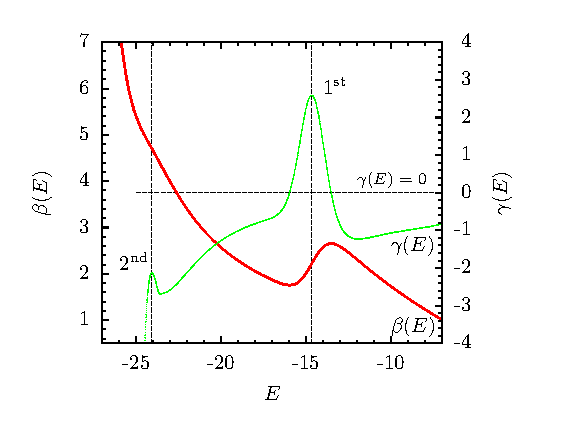
\includegraphics[width = 0.7\textwidth]{chapter2Figs/MicroAnalysisExample.eps}
\caption{\label{fig:Fig_1}%
Microcanonical inflection-point analysis of the inverse microcanonical temperature $\beta(E)$. The prominent back-bending region in $\beta(E)$, together with the positive-valued peak in its energy derivative $\gamma(E)$ at $E \approx -15$, indicates a first-order transition. The negative-valued peak at $E\approx -24$ corresponds to a second-order transition.}
\end{figure}
%

In analogy to the principle of minimal sensitivity~\cite{Stevenson}, structural transitions between pseudophases occur when $\beta(E)$, or one of its energy
derivatives, respond least sensitively to variations in energy\cite{Schnabel2011}. In particular, first-order transitions are associated with inflection points in $\beta (E)$ that have a positive slope, accompanied by positive-valued peaks in the energy derivative $\gamma(E)=d\beta(E)/dE$. Similarly, a second-order transition occurs when $\beta(E)$ exhibits an inflection point with a negative slope and $\gamma(E)$ attains a negative-valued peak. Examples of microcanonical pseudophase transition signals are shown in Fig.~\ref{fig:Fig_1}. The formalism can be naturally extended to higher-order transitions. Inflection point in the $(2\mathrm{n})$th-derivative of entropy, accompanied by a positive-valued valley in the $(2\mathrm{n}+1)$th-derivative, indicates a $(2\mathrm{n}+1)$th-order transition. Similarly, a $(2\mathrm{n})$th-order transition is marked by an inflection point in the $(2\mathrm{n}-1)$th-derivative of entropy and a negative-valued peak in the $(2\mathrm{n})$th-order derivative.

%
\begin{figure}
\center
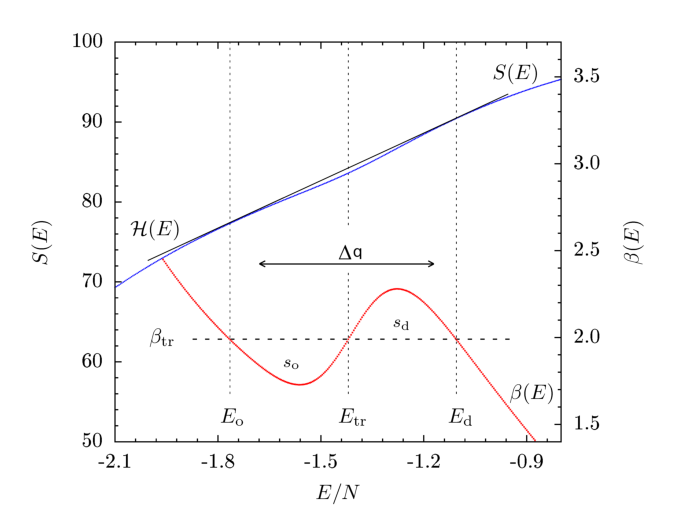
\includegraphics[width = 0.7\textwidth]{chapter2Figs/maxwellConstruct.eps}
\caption{\label{fig:Fig_2}%
The convex region of the microcanonical entropy $S(E)$ and the back-bending of the microcanonical inverse temperature $\beta(E)$ are prominent indicators of \textit{first-order} transitions. The slope of the double-tangent Gibbs hull $\mathcal{H}(E)$ defines the transition temperature $\beta_{\mathrm{tr}}$. The Maxwell construction, defined by equal areas of $s_{\mathrm{o}}$ and $s_{\mathrm{d}}$, is itself positioned at $\beta_{\mathrm{tr}}$. The transition energy $E_{\mathrm{tr}}$ indicates the location of the largest separation between $\mathcal{H}(E)$ and $S(E)$, which signifies maximal entropic suppression of the transition states. The latent heat $\Delta Q$ corresponds to the width of the transition region between $E_{\mathrm{d}}$ and $E_{\mathrm{o}}$.}
\end{figure}
%
Alternatively, in the case of first-order transitions, the transition temperature $\beta_{\mathrm{tr}}$ can be obtained by the means of the Maxwell construction which was originally introduced to repair the unphysical back-bending in the pressure versus volume isotherms for the van der Waals gas. In mesoscopic systems, the finite-size effects lead to the entropic suppression of transition states, which is manifested in the backbending of $\beta(E)$ and the convex intruder in $S(E)$. The position of the Maxwell construction is determined by the equality of the areas $s_{\mathrm{o}}$ and $s_{\mathrm{d}}$ [Fig.\ref{fig:Fig_2}]. Commonly referred to as \textit{surface entropies}, $s_{\mathrm{o}}$ and $s_{\mathrm{d}}$ are defined as the integrals
\begin{eqnarray}
\label{eq:surfaceEntr}
s_{\mathrm{o}} &=& \int_{E_{\mathrm{o}}}^{E_{\mathrm{tr}}} dE \:\: (\beta_{\mathrm{tr}}-\beta(E)), \\
s_{\mathrm{d}} &=& \int_{E_{\mathrm{tr}}}^{E_{\mathrm{d}}} dE \:\: (\beta(E)-\beta_{\mathrm{tr}}).
\end{eqnarray}
The Maxwell line intersects the inverse temperature at the energies $E_{\mathrm{o}}$, $E_{\mathrm{tr}}$, and $E_{\mathrm{d}}$. The latent heat
$\Delta Q = E_{\mathrm{d}} - E_{\mathrm{o}}$ corresponds to the energetic separation between the ordered and the disordered pseudophases . The transition energy $E_{\mathrm{tr}}$ indicates the location where intermediate states experience the maximal entropic suppression\cite{Bachmann2014}.

The slope of the double-tangent Gibbs construction, also shown in Figure \ref{fig:Fig_2}, provides yet another definition of $\beta_{\mathrm{tr}}$. As a function of energy, the Gibbs hull is defined as
\begin{equation}
\mathcal{H}(E) = S(E_{\mathrm{o}}) + \beta_{\mathrm{tr}}[E-E_{\mathrm{o}}],
\end{equation}
where $\beta_{\mathrm{tr}}$ can be expressed in terms of the energy and entropy differences between the ordered and disordered pseudophases as
\begin{equation}
\beta_{\mathrm{tr}} = \frac{S_{\mathrm{d}}-S_{\mathrm{o}}}{E_{\mathrm{d}}-E_{\mathrm{o}}} = \frac{\Delta S}{\Delta Q}.
\end{equation}
With the exception of composite multi-step transitions, characterized by additional oscillations in the back-bending region of $\beta(E)$, the transition temperatures obtained by the means of the Maxwell and Gibbs constructions are identical.

The formalism of the microcanonical inflection-point analysis makes no reference to the thermodynamic limit. In fact, it is equally suitable for analysis of macroscopic and mesoscopic systems alike. This is in stark contrast to the more traditional canonical analysis which is defined under the assumption of the thermodynamic limit and has to be modified for the treatment of finite systems.

 
 
\section{The canonical ensemble}
\label{sec:canonicalEnsemble}
The canonical ensemble describes the behavior of a closed system which is in thermal equilibrium with a large external heat bath at a fixed temperature $T$. In analogy to the density of states in the microcanonical ensemble, the partition function $Z(T)$ contains all the essential information about the thermodynamic properties of the system under consideration\cite{Landau2000}. It can be defined directly as a Laplace transform\footnote{Here we assume that the system under investigation has discrete energy levels, which is always true in the context of computational studies. In the case of a continuous energy spectrum, the discrete sum is replaced by the integral $Z(T) = \int dE \:\:  g(E) e^{-\frac{E}{k_{\mathrm{B}}T}}$.} of the microcanical density of states $g(E)$
\begin{equation}
Z(T) = \sum_{i} g(E_{i}) e^{-\frac{E_{i}}{k_{\mathrm{B}}T}},
\end{equation}
where $T$ is the canonical temperature and $k_{\mathrm{B}}$ is the Boltzmann constant. The condition of thermal equilibrium prohibits any net average energy transfer between the system and the heat bath. However, the system can temporarily gain or loose energy through constant fluctuations and dissipations. The probability for a given microstate $\mu$ at a temperature $T$ is given by the Boltzmann distribution
\begin{equation}
p(\mu) = \frac{1}{Z(T)}e^{-\frac{\mathcal{H}(\mu)}{k_{\mathrm{B}}T}},
\end{equation}
where $\mathcal{H}$ is the Hamiltonian of the system. The appropriate thermodynamic potential in the canonical ensemble is the Helmholtz free energy
\begin{equation}
F(T) = -k_{\mathrm{B}}T \: \mathrm{ln}\, Z(T).
\end{equation}
This quantity represents the energy available to perform work and can be used to obtain all other thermodynamic quantities by differentiation\cite{Pathria,Sethna2006}. The temperature derivative of the free energy defines the canonical entropy
\begin{equation}
\label{eq:canonicalEntropy}
S(T) = -\frac{\partial}{\partial T}F(T)\bigg|_{N,V},
\end{equation} 
which measures the amount of disorder in the system.
The internal energy $U$, defined as a sum over all microstate energies weighted by the Boltzmann distribution  
\begin{equation}
\label{eq:InternalEnergy}
U(T) = \frac{\sum_{\mu} \mathcal{H}(\mu)e^{-\frac{\mathcal{H}(\mu)}{k_{\mathrm{B}}T}}}{Z(T)} =  \frac{\sum_{E} E \, g(E) e^{-\frac{E}{k_{\mathrm{B}}T}}}{Z(T)},
\end{equation}
represents the average energy of the system. Alternatively, the internal energy can be obtained by the differentiation of the free energy
\begin{equation}
U(T) = k_{\mathrm{B}}T^{2}\frac{\partial}{\partial T} \mathrm{ln} Z(T)\bigg|_{N,V}
= -T^{2}\frac{\partial}{\partial T}\left(\frac{F}{T}\right)\bigg|_{N,V}.
\end{equation}
\newpage
\noindent
The amount of energy needed to increase the temperature of the system by one unit is given by the specific heat 
$C_{V}$, defined as a temperature derivative of the internal energy
\begin{equation}\label{eq:22}
C_{V}(T) = \frac{\partial}{dT}U(T)\bigg|_{N,V} = -T\frac{\partial^{2}}{\partial T^{2}}F(T)\bigg|_{N,V}.
\end{equation}
On the other hand, starting with the third term in equation \ref{eq:InternalEnergy} we obtain the following expression 
\begin{eqnarray}
C_{V}(T) &=&  \frac{\partial}{dT}\frac{\sum_{E} E \, g(E) e^{-\frac{E}{k_{\mathrm{B}}T}}}{Z(T)} = -\frac{1}{k_{\mathrm{B}}T^2}\frac{\partial}{\partial \beta}\frac{\sum_{E} E \, g(E) e^{-\beta E}}{\sum_{E}g(E) e^{-\beta E}} \nonumber \\
&=& \frac{1}{k_{\mathrm{B}}T^2} \left[\left(\frac{\sum_{E} E^{2} \, g(E)  e^{-\beta E}}{Z(T)}\right) - \left(\frac{\sum_{E} E \, g(E)  e^{-\beta E}}{Z(T)}\right)^{2}\right] \nonumber \\
&=& \frac{1}{k_{\mathrm{B}}T^2}\left(\left<E^{2}\right> - \left<E\right>^{2}\right),
\end{eqnarray}
where the last expression corresponds to the variance of the Boltzmann distribution. This result is of a profound physical importance, establishing the connection between the macroscopic response quantity $C_{V}$, and microscopic fluctuations.

\subsection{Canonical analysis of phase transitions}
Sudden dramatic changes of macroscopic properties, in response to small variations of an external control parameter, indicate that the system under investigation is undergoing a phase transition. Here we consider temperature-driven transitions and describe a classification scheme similar to Ehrenfest's.

In the thermodynamic limit, it is generally possible to identify some property of the system which is non-zero in the ordered phase and zero in the disordered phase, i.e. the order parameter\cite{Bachmann2014,Landau2000}. A standard example is the magnetization $m$ in a ferromagnetic system, where $m = 1$ in the ordered ferromagnetic phase and $m = 0$ in the disordered paramagnetic phase. The derivative of the order parameter with respect to its conjugate variable defines a response quantity\footnote{In the case of the magnetization $m$, the appropriate conjugate thermodynamic variable is the external field $H$, and the corresponding response quantity is the magnetic susceptibility $\chi$.} which is discontinuous at the transition point. Order parameters also play a central role in the formulation of the Landau theory, where they serve as a basis for the expansion of the free energy around the transition point\cite{Kardar2009}. 

\begin{figure}
\center
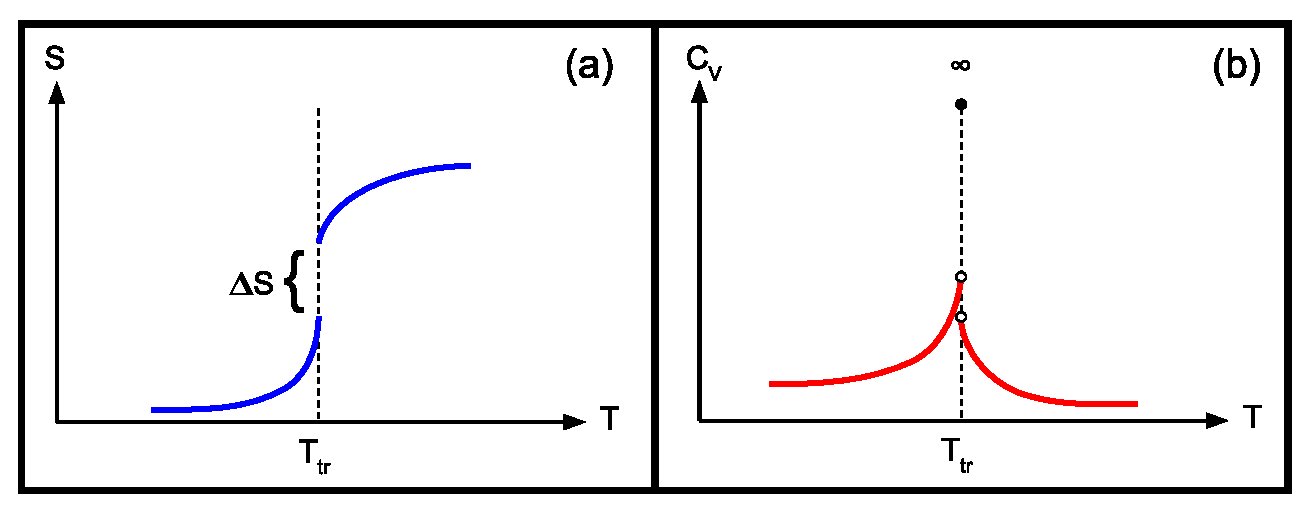
\includegraphics[width = 0.8\textwidth]{chapter2Figs/CanonicalFirstOrder.eps}
\caption{\label{fig:Fig_3}% 
(a) The jump discontinuity in the canonical entropy $S$, (b) and the delta peak in the specific heat $C_{V}$, are characteristic of a first order phase transition.}
\end{figure} 

First order transitions are characterized by a jump discontinuity $\Delta S$ in entropy and the coexistence of two distinct phases\footnote{As a familiar example, consider the coexistence of gas bubbles and liquid at the boiling point of water.} at the transition temperature. The energetic separation between the two phases corresponds to the latent heat
\begin{equation}
\Delta Q = T_{\mathrm{trans}}\,\Delta S,
\end{equation}
where $\Delta S$ is the height of the discontinuity and $T_{\mathrm{trans}}$ is the transition temperature. The specific heat $C_{V}$ exhibits a delta peak at $T_{\mathrm{trans}}$, as shown in Fig. \ref{fig:Fig_3}\,(b).

\newpage

\begin{figure}
\center
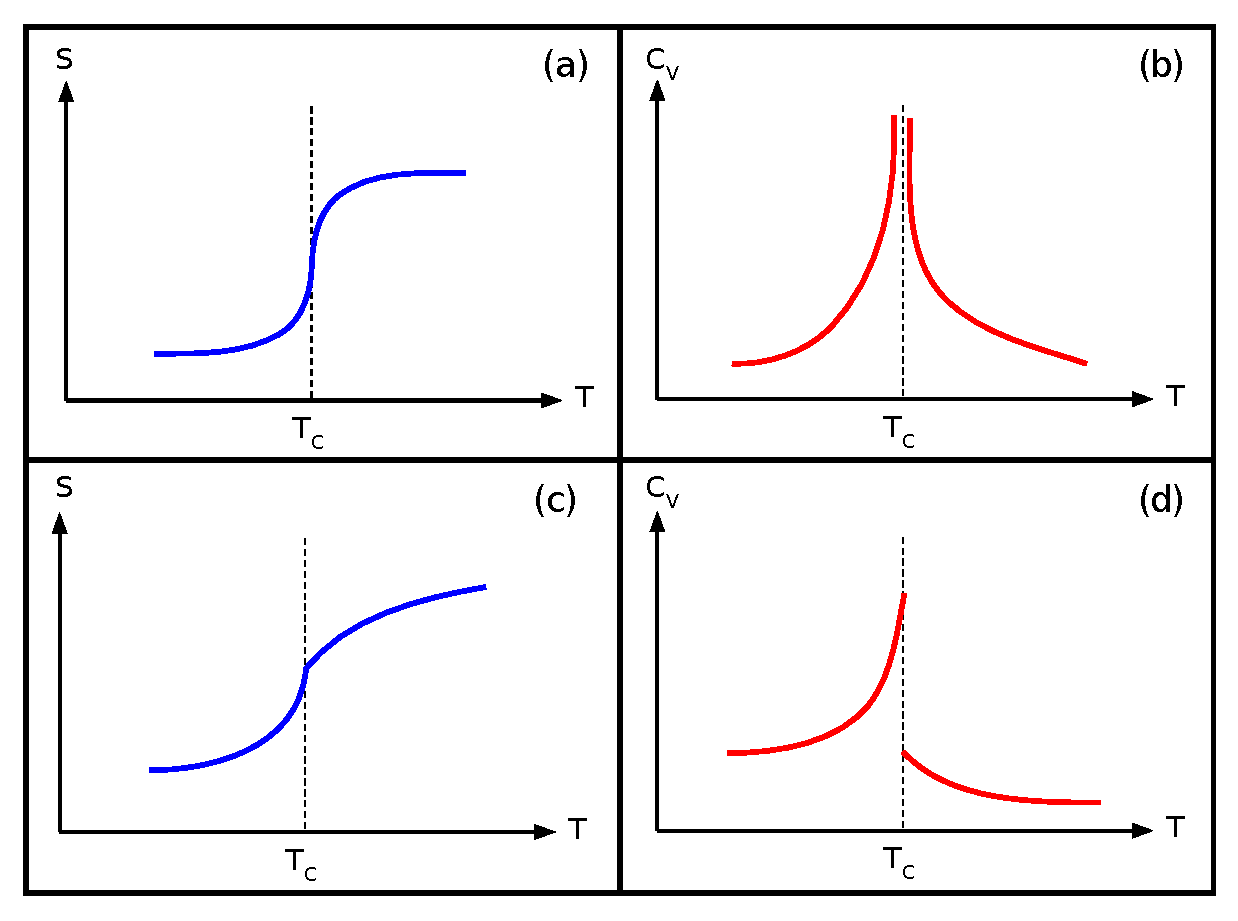
\includegraphics[width = 0.75\textwidth]{chapter2Figs/CanonicalSecondOrder.eps}
\caption{\label{fig:Fig_4}% 
Second order transitions are characterized by discontinuities in response quantities, such as the specific heat. (a,b) In the case of a \textbf{critical} second order transition, the entropy $S$ attains an infinite slope at $T_{c}$ accompanied by a divergence in the specific heat $C_{V}$. (c,d) So called \textit{lambda} transitions are characterized by a jump discontinuity in $C_{V}$ and a cusp singularity in entropy.}
\end{figure}

Second order transitions do not posses discontinuities in entropy, and for that reason are often called \textit{continuous} transitions. Instead, discontinuities are found in the second derivatives of the free energy with respect to temperature. It is customary to make use of equation\,\,\ref{eq:22}, and consider the specific heat $C_{V}$ which also contains the same discontinuities.
In the vicinity of the transition point $T_{c}$, the specific heat exhibits a power law behavior $C_{V}(\tau) \propto \left| \tau \right|^{-\alpha}$, where $\tau = \left(T-T_{c}\right)/T_{c}$ and $\alpha$ is the associated critical exponent. Examples of common types of discontinuities of $C_{V}$ are shown in Fig. \ref{fig:Fig_4}. Other important quantities such as the magnetic susceptibility $\chi$ and the correlation length $\xi$ also exhibit a power law behavior near the transition point, governed by the critical exponents $\gamma$ and $\nu$ respectively. The striking observation, that in the vicinity of the critical temperature $T_{c}$, the behavior of physical systems with diverse microscopic properties can be described in terms of the same critical exponents, is formalized in the theory of Universality\cite{Kardar2009}. 

\subsubsection{Canonical analysis in mesoscopic systems} 
The description of phase transitions in the terms of discontinuities and divergences is valid only in the thermodynamic limit. In situations where the thermodynamic behavior of a system is affected by finite size effects, this idealized description no longer applies. Nevertheless, the numerous examples of abrupt changes of macroscopic properties in finite systems necessitate the generalization of the theory. In order to avoid possible confusion, we shall refer to significant conformational changes in finite systems as \textit{pseudophase transitions}. Similarly, sets of macrostates with sufficiently similar macroscopic properties will be denoted \textit{pseudophases}.

In the generalized formalism, peaks in the specific heat and other response quantities indicate regions of increased thermodynamic activity, i.e. pseudophase transitions. The order of the transition is determined from the shape of the canonical energy distribution in the transition region. Bimodal distributions reveal the coexistence of two pseudophases and indicate a first-order transition\cite{Janke1998}. The associated latent heat of the transition is given by the energetic separation between the two peaks in the distribution. Second-order transitions correspond to unimodal energy distributions. The power law behavior of response quantities contains significant finite-size corrections and in some cases is altogether not applicable\cite{Landau2000}. An example of canonical analysis, applied to first- and second-order pseudophase transitions, is illustrated in Fig. \ref{fig:Fig_5}. 

\begin{figure}
\center
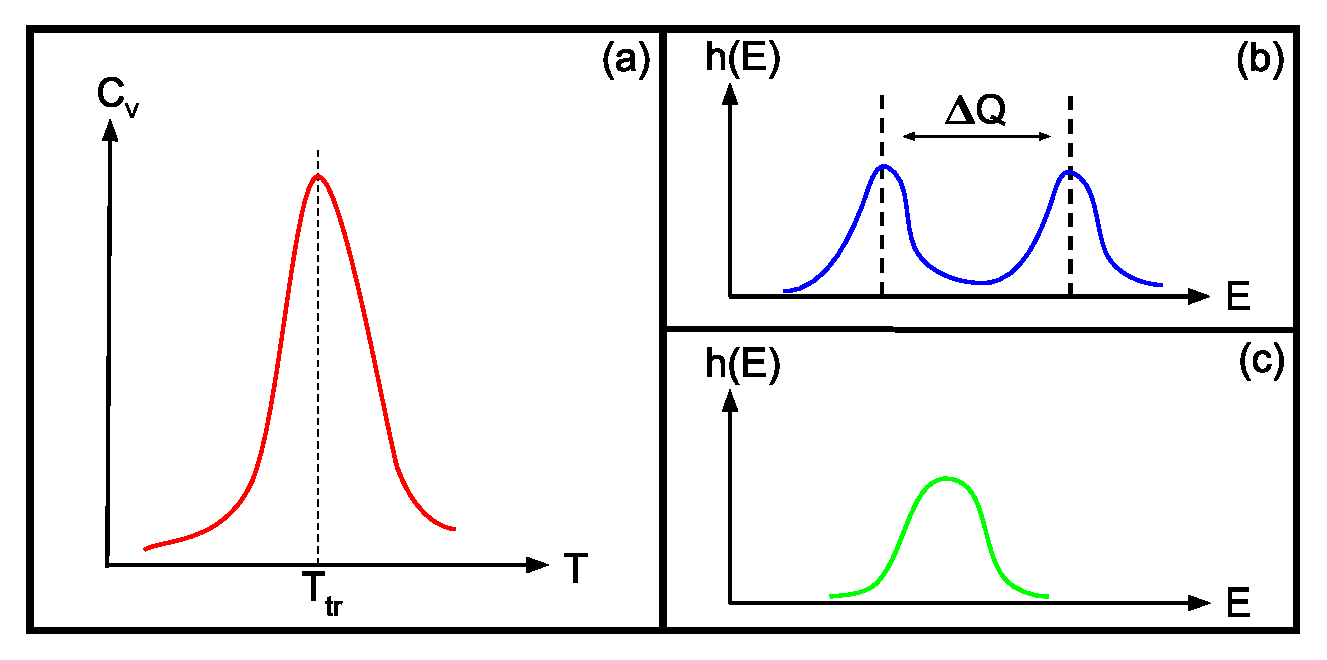
\includegraphics[width = 0.8\textwidth]{chapter2Figs/CanonicalAnalysisSample.eps}
\caption{\label{fig:Fig_5}% 
(a) The peak in the specific heat $C_{V}$ indicates a region of heightened thermodynamic activity. (b) The two peaks in the bimodal canonical energy distribution correspond to the ordered and disordered pseudophases, energetically separated by the latent heat $\Delta Q$. Pseudophase coexistence and latent heat are reliable indicators of a first-order pseudophase transition. (c) Second-order transitions are marked by wide unimodal energy distributions at the transition point.}
\end{figure}

It should be mentioned that second-order pseudophase transitions do not always produce peaks in the specific heat. In general, it is necessary to investigate the behavior of several response quantities in order to obtain an accurate picture of the transition properties of the system under investigation. However, due to finite size effects, the signals obtained from different quantities will in general not coincide at a single transition temperature. This reality further fortifies the argument that the microcanonical inflection-point analysis\footnote{Introduced in Sec. \ref{subsec: micro_analysis}}, which defines a unique transition temperature in mesoscopic and macroscopic systems alike, is the preferred formalism for the analysis of finite systems.
\newpage

\section{Alternative definitions of the density of states}
In section \ref{sec:mic_ensemble} we have defined the microcanonical density of states $g(E)$ as an integral over the surface of constant energy in the $6N$-dimensional phase space. We have argued that $g(E)$ contains all the essential information about the thermodynamic properties of the system under consideration, and introduced the formalism of the microcanonical inflection-point analysis which uses the logarithm of $g(E)$ as its starting point. In section \ref{sec:canonicalEnsemble} we have shown that the canonical partition function $Z(T)$ can be obtained by performing a Laplace transform of $g(E)$. Clearly, the microcanonical density of states plays a fundamental role in equilibrium statistical mechanics, and as such needs to be carefully defined. 

Two distinct definitions of the density of states arise from certain ambiguity in the exact meaning of the microcanonical ensemble in computational studies. The density of states can be defined in the context of the conformational microcanonical ensemble $(N,V,E_{p})$ as a function of the potential energy only
\begin{equation}
g_{c}(E_{p}) = \int \mathcal{DQ} \:\: \delta(E_{p} - \mathcal{H}(\mathcal{Q}))
\end{equation}
This definition is commonly used in Monte Carlo simulations of magnetic systems where the kinetic energy contributions have little physical significance and the sampling can be restricted to the conformational space. However, in systems where the transfer between potential and kinetic energy has important physical interpretation, the sampling of the full phase space becomes necessary. The standard definition of the microcanonical ensemble $(N,V,E)$ is applied and the measured density of states becomes a function of the total system energy, which can be written as the sum of the potential and kinetic energies
\begin{equation}
E = E_{p} + E_{k}.
\end{equation}
In order to distinguish between the two definitions, we shall use the symbol $\Gamma(E)$ to represent the latter definition of the density of states. The connection between the conformational density of states and $\Gamma(E)$ is expressed as a convolution\cite{Calvo1995}
\begin{equation}
\label{eq:TotalDOS}
\Gamma(E) = \int dE_{k} \: g_{c}(E - E_{k})g_{k}(E_{k}),
\end{equation}
where 
\begin{equation}
g_{k}(E_{k}) = \int \mathcal{DP} \:\: \delta(E_{k} - \mathcal{H}(\mathcal{P}))
\end{equation}
is the kinetic density of states obtained by integrating over the momentum space.

We shall now turn our attention to the consequence of choosing either the conformational or the full density of states as the starting point for a systematic analysis of the thermodynamic properties of a system under consideration. In the following we will discuss the impact of ignoring the momentum degrees of freedom on the results of both the canonical and microcanonical analysis. As an illustration, we will provide results from Monte Carlo simulations of two short flexible homopolymers.

\subsection{Consequences for canonical analysis}
The canonical partition function $Z(T)$ and the microcanonical density of states are connected via a Laplace transform. We begin with the full density of states $\Gamma(E)$ and using the definition from Eq. \ref{eq:TotalDOS} write
\begin{equation}
\label{eq:Laplace}
Z(T) = \mathcal{L}\left\lbrace\Gamma(E)\right\rbrace = \mathcal{L}\{g_{c} \ast g_{k} \} = \mathcal{L}\{g_{c}\} \mathcal{L}\{g_{k}\},
\end{equation}
where the last step follows from the convolution theorem\cite{Arfken}. 
\newpage
\noindent
The partition function of the system can hence be conveniently written as a product of two independent partition functions
\begin{equation}
Z(T) = Z_{c}(T)Z_{k}(T),
\end{equation}
which depend on the potential and kinetic energies respectively. It follows that the average ensemble energy can be expressed as the sum of the average potential and kinetic energies
\begin{eqnarray}
U(T)  &=& k_{\mathrm{B}}T^{2}\frac{\partial}{\partial T} \mathrm{ln} Z\bigg|_{N,V} \nonumber \\
	 &=& k_{\mathrm{B}}T^{2}\frac{\partial}{\partial T} \mathrm{ln} Z_{c} \bigg|_{N,V}	 + k_{\mathrm{B}}T^{2}\frac{\partial}{\partial T} \mathrm{ln} Z_{k} \bigg|_{N,V}	 \nonumber \\
	 &=& \langle E_{c} \rangle + \langle E _{k}\rangle.  
\end{eqnarray}
With the exception of systems with rigid constraints, the average kinetic energy is given by the equipartition theorem 
\begin{equation}
 \langle E _{k}\rangle = \frac{3Nk_{\mathrm{B}}T}{2},
\end{equation}
where $N$ is the number of particles in the system. It follows that the specific heat $C_{\mathrm{V}}$ obtains only a trivial additive constant from the kinetic energy term
\begin{eqnarray}
C_{\mathrm{V}}(T) &=& \frac{\partial}{\partial T} U(T)\bigg|_{N,V} \nonumber \\
				 &=& \frac{\partial}{\partial T} \langle E_{c} \rangle\bigg|_{N,V} + \frac{\partial}{\partial T}\frac{3Nk_{\mathrm{B}}T}{2} \nonumber \\
				 &=& C_{\mathrm{V},\mathrm{conf.}} + \frac{3Nk_{\mathrm{B}}}{2}.
\end{eqnarray}

\begin{figure}
\center
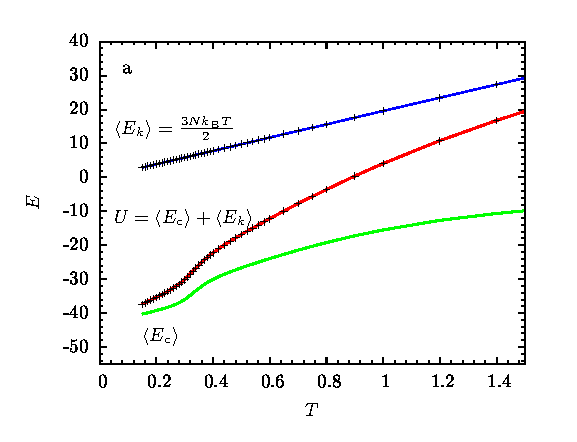
\includegraphics[width = 0.49\textwidth]{chapter2Figs/N13Energy.eps}
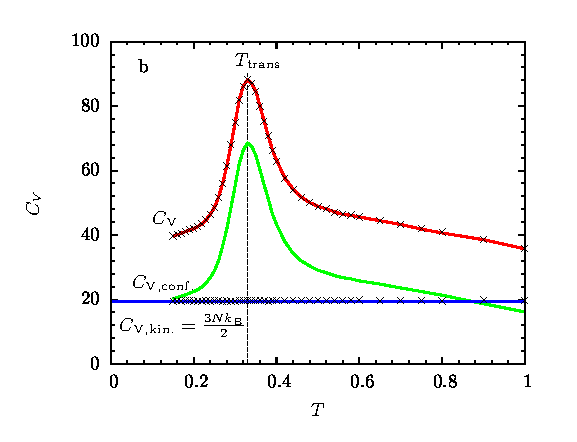
\includegraphics[width = 0.49\textwidth]{chapter2Figs/N13Spec.eps}
\caption{\label{fig:Fig_6}% 
Results of a Monte Carlo simulation of a short flexible homopolymer of length $N=13$. The average kinetic energy $\langle E _{k}\rangle$ and the kinetic contributions $C_{\mathrm{V,kin.}}$ towards the specific heat are plotted as points on top of their respective theoretical curves (blue). The average potential energy $\langle E_{c} \rangle$ and the configurational specific heat $C_{\mathrm{V},\mathrm{conf.}}$ (green) were obtained by sampling of the configurational space. Sampling of the full phase space was performed to obtain the total average energy $U$ and the combined specific heat $C_{\mathrm{V}}$ (red). As expected, the combined specific heat is identical to $C_{\mathrm{V},\mathrm{conf.}}$, except for a trivial additive constant.}
\end{figure}

In conclusion, the locations and shapes of signals for pseudophase transitions are not affected by the inclusion of the momentum space into a sampling scheme. To substantiate this assertion, in Fig. \ref{fig:Fig_6} we present the results from a Monte Carlo study of a short flexible homopolymer. The average kinetic energy $\langle E _{k}\rangle$ and the kinetic contributions $C_{\mathrm{V,kin.}}$ towards the specific heat are plotted as points on top of their respective theoretical curves (blue), showing good agreement with the predicted values. The average potential energy $\langle E_{c} \rangle$ and the configurational specific heat $C_{\mathrm{V},\mathrm{conf.}}$ (green) were obtained by the sampling of the configurational space only. Sampling of the full phase space was performed to obtain the total average energy $U$ and the combined specific heat $C_{\mathrm{V}}$ (red). As expected, the combined specific heat is identical to $C_{\mathrm{V},\mathrm{conf.}}$, except for a trivial additive constant. The estimate of the transition temperature is independent of the choice of either definition of the density of states. 
\newpage 

\subsection{Consequences for microcanonical analysis}
The application of the Laplace transform to the total density of states $\Gamma (E)$, allowed us to conveniently disentangle the convolution in Eq.\,\,\ref{eq:TotalDOS} \, into separate kinetic and conformational contributions [Eq. \ref{eq:Laplace}]. Unfortunately, in the microcanonical ensemble no such simplification is readily available. Let us however consider a class of physical systems whose momenta and positional degrees of freedom are independent. Explicit integration over the momentum space yields a simple expression for the kinetic density of states
\begin{equation}
g_{k}(E_{k}) = \int \mathcal{DP} \:\: \delta(E_{k} - \mathcal{H}(\mathcal{P})) 
			 = E_{k}^{\frac{3N-2}{2}}.
\end{equation}
Combining the result with Eq. \ref{eq:TotalDOS} \, we obtain
\begin{equation}
\Gamma(E) = \int dE_{k} \: g_{c}(E - E_{k})E_{k}^{\frac{3N-2}{2}}.
\end{equation}
Next, taking a derivative with respect to the total energy $E$ and dividing both sides by $\Gamma(E)$ we get two equivalent expressions for the microcanonical inverse temperature 
\begin{eqnarray}
\beta(E) &=& \int dE_{k} \:\frac{3N-2}{2E_{k}} \:\left[\frac{g_{c}(E - E_{k})E_{k}^{\frac{3N-2}{2}}}{\Gamma (E)}\right]
\label{eq:beta1}  \\
		&=& \int dE_{p} \: \beta_{c}(E_{p})\: \left[ \frac{g_{c}(E_{p})(E- E_{p})^{\frac{3N-2}{2}}}{\Gamma (E)} \right]
\label{eq:beta2}.  
\end{eqnarray}
Recognizing the two terms enclosed in square brackets as the microcanonical probability densities for the kinetic and potential energies,
we can rewrite equations \ref{eq:beta1} and \ref{eq:beta2} as
\newpage
\noindent
\begin{equation}
\label{eq:beta3}
\beta(E) = \int dE_{k} \:\frac{3N-2}{2E_{k}} \: \rho(E_{k})_{E} = \frac{3N-2}{2}\left\langle \frac{1}{E_{k}}  \right\rangle,
\end{equation}
and 
\begin{equation}
\label{eq:beta4}
\beta(E) = \int dE_{p} \: \beta_{c}(E_{p})\: \rho(E_{p})_{E} = \left\langle \beta_{c} \right\rangle.
\end{equation}
The microcanonical inverse temperature, obtained by the differentiation of the total density of states, can therefore be interpreted as an average of the conformational and kinetic anologs weighted by their respective microcanonical probability distributions.

When the number of particles in the system is large, the probability densities $\rho(E_{k})_{E}$ and $\rho(E_{p})_{E}$ are expected to be sharply peaked around the most probable kinetic $\bar{E}_{k}$ and potential $\bar{E}_{p}$ energies respectively . We can therefore apply the saddle point approximation to the integrals in equations [\ref{eq:beta3}, \ref{eq:beta4}] and obtain the following first order approximations for the inverse temperature
\begin{equation}
\label{eq:approx1}
\beta(E) \approx \beta_{c}(\bar{E}_{p}),
\end{equation}
and
\begin{equation}
\label{eq:approx2}
\beta(E) \approx \frac{3N-2}{2}\left(\frac{1}{\bar{E}_{k}}\right). 
\end{equation}
The first expression suggests that it is possible to reconstruct $\beta(E)$ from the conformational inverse temperature $\beta_{c}$, and that the two quantities contain essentially the same information. We test the validity of this hypothesis by comparing the microcanonical results of Monte Carlo simulations of a flexible elastic $55-$mer, which were carried out in both the conformational space and the full phase space.
\newpage
\begin{figure}
\center
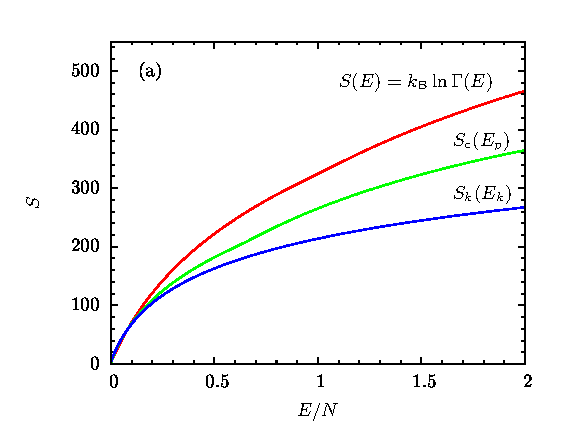
\includegraphics[width = 0.49\textwidth]{chapter2Figs/N55Entropy.eps}
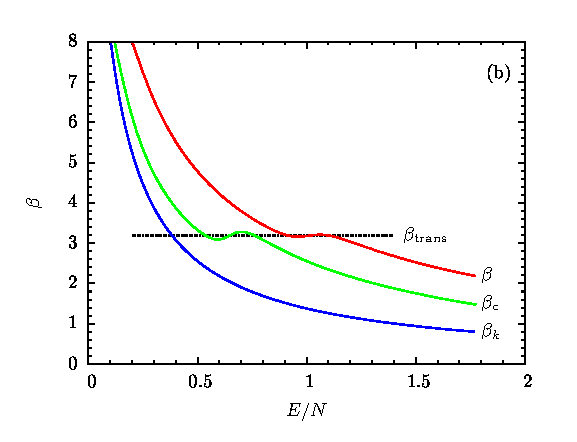
\includegraphics[width = 0.49\textwidth]{chapter2Figs/N55Beta.eps}
\caption{\label{fig:Fig_7}% 
Comparison of microcanonical results from a Monte Carlo simulation of a flexible homopolymer of length $N=55$.(a) The combined $S$, conformational $S_{c}$, and kinetic $S_{k}$ entropy curves. (b) The kinetic inverse temperature $\beta_{k}$ is a strictly convex function and the application of the inflection-point analysis reveals no transition signals. The conformational inverse temperature $\beta_{c}$ clearly differs from $\beta(E)$, however both indicate a first-order pseudophase transition at virtually the same temperature. }
\end{figure}
The kinetic entropy in Fig. \ref{fig:Fig_7} is a strictly concave function and the application of the inflection-point analysis to the corresponding inverse temperature $\beta_{k}$ reveals no transition signals. The conformational inverse temperature clearly differs from $\beta(E)$, however both indicate a first-order pseudophase transition at virtually the same temperature. In Fig. \ref{fig:Fig_8} we show the comparison between the true $\beta(E)$ and the reconstruction obtained from the conformational inverse temperature according to equations \ref{eq:approx1} and \ref{eq:approx2}. It is evident that the approximation is valid, except in the back-bending region of the first-order transition due to the bimodality of the probability densities $\rho(E_{k})_{E}$ and $\rho(E_{p})_{E}$. 

\newpage
The expression in equation \ref{eq:approx2} can be rewritten as 
\begin{equation}
k_{\mathrm{B}}T(E) \approx \frac{2}{3N-2}\left(\frac{1}{\bar{E}_{k}}\right)^{-1},
\end{equation}
which clearly resembles the well known relationship between the canonical temperature and the average kinetic energy. In the the thermodynamic limit, this approximation becomes exact and the equivalency of the microcanonical and canonical ensembles is restored. 



\begin{figure}
\center
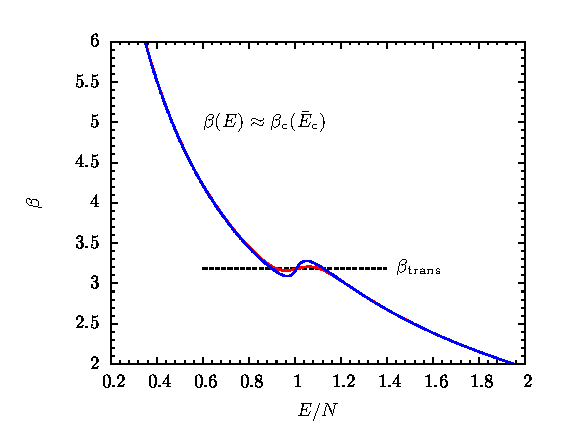
\includegraphics[width = 0.7\textwidth]{chapter2Figs/N55BetaComp.eps}
\caption{\label{fig:Fig_8}% 
Comparison of the inverse microcanonical temperature $\beta(E)$ (red) and the conformational inverse temperature $\beta_{c}(\bar{E}_{p})$ (blue) evaluated at the most probable potential energy $\bar{E}_{p}$. The approximation introduced in equation \ref{eq:approx1} holds except in the back-bending region of the first-order pseudophase transition. The inverse transition temperature $\beta_{\mathrm{trans}}$ obtained from the two quantities is virtually identical.}
\end{figure}

%%%%%%%%%%%%%%%%%%%%%%%%%%%%%%%%%%%%%%%%%%%%%%%%%%%%%%%%%%%%%%%%%%%%%%%%%%%%%%%%%%%%
%%%%%%%%%%%%%%%%%% 			CHAPTER 3     		%%%%%%%%%%%%%%%%%%%%%%%%%%%%%%%%%%%
%%%%%%%%%%%%%%%%%%%%%%%%%%%%%%%%%%%%%%%%%%%%%%%%%%%%%%%%%%%%%%%%%%%%%%%%%%%%%%%%%%%%

\chapter{Computational Methods}

Computational algorithms are powerful tools that enable the investigation of  many-body physical systems under thermal conditions, that are far too complex to be solved analytically.
In fact, only a handful of systems with large number of degrees of freedom are exactly solvable\footnote{The most prominent examples of exactly solvable systems with large number of degrees of freedom are the ideal gas and the two dimensional Ising model.}, and even the simplest solutions often require bewildering mathematical gymnastics. Consequently, computational studies are the main source of advances in the fundemental understanding of complex microscopic and mesoscopic systems such as biopolymers and proteins \cite{Bachmann2014}.

Two complementary classes of computational algorithms have been particularly successful in unravelling the thermodynamic properties of physical systems. \textit{Molecular dynamics} simulations generate a single phase space trajectory by updating the positions and momenta of every particle in a system according to Hamilton's equations \cite{Rapaport2004,Tuckerman2010}. Alternatively, carrying out a stochastic sampling of the phase space, \textit{Monte Carlo} simulations estimate the equilibrium properties without an explicit consideration of the system's dynamics \cite{Bachmann2014, Landau2000}. In this chapter, we shall focus our attention to Markov chain Monte Carlo methods. We will briefly discuss the essential theory and introduce the well established Metropolis and Parallel Tempering algorithms as well as the lesser known Multiple Gaussian modified ensemble method.



\section{Markov chain Monte Carlo}
The aim of all Monte Carlo methods is to extract the equilibrium thermodynamic properties of physical systems by performing an efficient stochastic sampling of the phase space. For this purpose, a set of random microstates $\{\mu_{1},\mu_{2},...,\mu_{M}\}$ is generated according to some previously known probability distribution $p(\mu_{i})$, and the expectation value for any observable $O({\mu})$ is estimated by calculating the average
%
\begin{equation}
\label{eq:expectationValue}
\bar{O} = \frac{1}{M}\sum_{i = 1}^{M} O(\mu_{i}).
\end{equation}
%
In most Monte Carlo methods, the set of random microstates is generated according to a discrete-time Markov chain (DTMC) \cite{Resnick2005}. Markov chains are sequences of random states, generated according to the time-independent transition probabilities $T(\mu \rightarrow \nu)$ which satisfy the Markov property. In simple terms, the probability of moving to state $\nu$ from state $\mu$ depends only on the present state, and is independent of the history of the process. In order to achieve the correct statistical sampling of an equilibrium thermodynamic ensemble, the following conditions must also be satisfied.

The process must be \textbf{ergodic}, i.e., there must be a path of non-zero probability between any pair of states. More formally, the state space $\mathcal{S}$ of the Markov chain must consist of a single aperiodic recurrence class. When ergodicity is satisfied, the ensemble average $\left\langle O \right\rangle$ can be approximated by the measured expectation value $\bar{O}$ [Eq. \ref{eq:expectationValue}] 
%
\begin{equation}
\label{eq:approximationOfExpectationValues}
\bar{O} = \frac{1}{M}\sum_{i = 1}^{M} O(\mu_{i}) \approx \left\langle O \right\rangle = \int \mathcal{DP}\mathcal{DQ} \:\: O(\mathcal{P},\mathcal{Q})
p(\mathcal{P},\mathcal{Q}),
\end{equation}
%
where $M$ is the length of the Markov chain. According to the ergodic hypothesis \cite{Tuckerman2010}, the approximation becomes exact in the limit of an infinitely long Markov chain
%
\begin{equation}
\label{eq:ergodicHyp}
\lim_{M\rightarrow \infty}\frac{1}{M}\sum_{i = 1}^{M} O(\mu_{i}) = \int \mathcal{DP}\mathcal{DQ} \:\: O(\mathcal{P},\mathcal{Q})
p(\mathcal{P},\mathcal{Q}).
\end{equation}
%
%
The time evolution of a discrete-time Markov process is described by the master equation
%
\begin{equation}
\label{eq:MasterEquation}
\frac{\Delta p(\mu)}{\Delta t} = \sum_{\nu} p(\nu)T\left(\nu \rightarrow \mu\right) - p(\mu)T\left(\mu \rightarrow \nu\right).
\end{equation}
%
The equilibrium condition requires that the probability distribution $p(\mu)$ is stationary. In other words, the probability currents into and out of the state $\mu$ must be always equal
\begin{equation}
\label{eq:balance}
\sum_{\nu} p(\nu)T\left(\nu \rightarrow \mu\right) = \sum_{\nu} p(\mu)T\left(\mu \rightarrow \nu\right).
\end{equation}
%
Also known as the $\textbf{balance}$ condition, equation \ref{eq:balance} sometimes allows for solutions that are not permitted in the equilibrium ensemble \cite{Landau2000}. The stricter condition of $\textbf{detailed balance}$ requires that the probability of a transfer between any two states must be equal to the probability of the reverse process. Embodied in the expression
%
\begin{equation}
\label{eq:detailedBalance}
p(\mu)T\left(\mu \rightarrow \nu\right) = p(\nu)T\left(\nu \rightarrow \mu\right),
\end{equation} 
%
this condition is sufficient to prevent any non-physical solutions as well as to ensure that the process is invariant under time reversal.


Having introduced the conditions of ergodicity and detailed balance, we can now derive the expression for transition probabilities which will ensure correct stochastic sampling according to an equilibrium distribution $p\left(\mu\right)$. 
For convenience, we will separate the transition probabilities into two separate terms and write


%
\begin{equation}
\label{eq:factoredTransitionProb}
T\left(\mu \rightarrow \nu\right) = s\left(\mu \rightarrow \nu\right)a\left(\mu \rightarrow \nu\right).
\end{equation}
Assuming the current state $\mu$, the probability of generating a new state $\nu$ is given by the selection probability $s\left(\mu \rightarrow \nu\right)$, while the probability of accepting the proposed update is controlled by the \textit{acceptance} probability $a\left(\mu \rightarrow \nu\right)$. Combining equations \ref{eq:detailedBalance} and \ref{eq:factoredTransitionProb}, we express the ratio of the transition probabilities as
%
\begin{equation}
\label{eq:ratioOfTransitionProb}
\frac{T\left(\mu \rightarrow \nu\right)}{T\left(\nu \rightarrow \mu\right)} = \frac{s\left(\mu \rightarrow \nu\right)a\left(\mu \rightarrow \nu\right)}{s\left(\nu \rightarrow \mu\right)a\left(\nu \rightarrow \mu\right)} = \frac{p\left(\nu\right)}{p\left(\mu\right)}.
\end{equation}
%
The ratio of the forward and backward selection probabilities
$\sigma(\mu,\nu) = s\left(\mu \rightarrow \nu\right)/s\left(\nu \rightarrow \mu\right)$
depends on the choice of the particular update scheme. In the remainder of this thesis, we shall assume that the forward and backward selection probabilities are equal and the ratio equals to unity, which is valid for most local Monte Carlo updates. This simplifying assumption allows us to rewrite equation \ref{eq:ratioOfTransitionProb} without making explicit references to the selection probabilities
%
\begin{equation}
\label{eq:acceptanceProbs}
\frac{a\left(\mu \rightarrow \nu\right)}{a\left(\nu \rightarrow \mu\right)} = \frac{p\left(\nu\right)}{p\left(\mu\right)}.
\end{equation}
%

\subsection{Metropolis sampling}

Any set of acceptance probabilities which satisfies equation \ref{eq:acceptanceProbs} is allowable, however the standard choice is to set the higher of the two probabilities to unity. This yields the well known Metropolis acceptance criterion \cite{Landau2000,Metropolis1953}:
%
\begin{equation}
\label{eq:MetropolisCriterion}
a\left(\mu \rightarrow \nu\right) = \mathrm{min}\left(1,\frac{p\left(\nu\right)}{p\left(\mu\right)} \right).
\end{equation}
% 
Under most circumstances, Metropolis sampling is carried out according to the canonical microstate probability distribution $p(\mu) \propto e^{-\beta E(\mu)}$, where $\beta$ is the inverse canonical temperature. Hence the acceptance probability is governed by the energy difference between the proposed and the current states
%
\begin{equation}
\label{eq:MetropolisCriterionCanonical}
a\left(\mu \rightarrow \nu\right) = \mathrm{min}\left(1,\frac{e^{-\beta E(\nu)}}{e^{-\beta E(\mu)}} \right) = \mathrm{min}\left(1,e^{-\beta \Delta E} \right).
\end{equation}
%
The average of the observable $O(\mu)$, measured over the length of a finite Metropolis run, serves as an estimate for the canonical expectation value $\left\langle O \right\rangle$ [Eq.\,\,\ref{eq:approximationOfExpectationValues}]. 
In the limit of an infinite run, this approximation becomes exact [Eq.\,\,\ref{eq:ergodicHyp}]. However, since all simulations are of finite length, it is imperative to account for the statistical errors introduced due to the finiteness of the measured data sets. The standard bias corrected error estimator for the calculated average $\bar{O}$, obtained from a finite set of $M$ uncorrelated measurements, is written as
%
\begin{equation}
\mathrm{err}(\bar{O}) = \pm \,\,\sqrt{\frac{1}{M(M-1)} \sum_{m} (O_{m} - \bar{O})^{2}}.
\end{equation}
%
In reality, most measurements obtained from Monte Carlo simulations are correlated. Hence it is necessary to introduce the modified error estimator
%
\begin{equation}
\mathrm{err}(\bar{O}) = \pm \,\,\sqrt{\frac{1}{M(M_{\mathrm{eff}}-1)} \sum_{m} (O_{m} - \bar{O})^{2}},
\end{equation}
%
where $M_{\mathrm{eff}}$ is the number of uncorrelated measurements\footnote{For detailed description of the more practical \textit{binning} and \textit{jackknife} error estimation methods, please refer to chapter 4 in \cite{Bachmann2014}.}.

The Metropolis method provides the means for an efficient sampling of microstates which are dominant at a given temperature. However, the microstates which are found in the tails of the canonical energy distribution are rarely visited. Further shortcomings of the Metropolis algorithm, such as the propensity for getting trapped in low-energy configurations and the notorious reduction in sampling efficiency near pseudophase transitions, motivate the introduction of more efficient sampling methods.


\subsection{Parallel tempering}
\label{subsec:ParallelTempering}
In situations where the Metropolis method fails to produce data of reasonable quality, the standard way of increasing sampling efficiency is to perform the simulation in a conveniently chosen \textit{generalized ensemble}\footnote{The microstate probability distribution of a generalized ensemble can be arbitrary and does not have to bear any resemblance to the Boltzmann distribution.}. In parallel tempering \cite{sw1,geyer1,huku1,huku2}, multiple canonical ensembles with different inverse temperatures $\{\beta_{1} < \beta_{2} < ... < \beta_{N}\}$ are simulated in parallel according to the standard Metropolis scheme. In this context, the generalized ensemble is defined as the direct product of $N$ canonical ensembles, and the partition function is given by
%
\begin{equation}
Z_{\mathrm{PT}}(\beta_{1},\beta_{2},...,\beta_{N}) = \prod_{i=1}^{N} Z_{\mathrm{can}}(\beta_{i}).
\end{equation}
%
At judiciously chosen intervals, an exchange of conformations between adjacent temperature threads $i$ and $j$ is proposed. The combined probability for states $(\mu, \, \nu)$ at respective temperatures $(\beta_{i}, \, \beta_{j})$ is given by
\begin{equation}
p_{\mu\nu} =  \frac{\displaystyle e^{-\beta_{i}E(\mu)}}{\displaystyle Z_{\mathrm{can}}(\beta_{i})} \frac{\displaystyle e^{-\beta_{j}E(\nu)}}{\displaystyle Z_{\mathrm{can}}(\beta_{j})},
\end{equation}
%
and the acceptance probability for the exchange of conformations is obtained from Eq. \ref{eq:MetropolisCriterion}
%
\begin{eqnarray}
\label{eq:replicaExchange}
a\left(\mu \leftrightarrow \nu;\beta _{i}, \beta_{j} \right) &=&
\mathrm{min}\left(1, \frac{\displaystyle e^{-\beta_{i}E(\nu)}e^{-\beta_{j}E(\mu)}}{\displaystyle e^{-\beta_{i}E(\mu)}e^{-\beta_{j}E(\nu)}}\right) \nonumber \\
&=&
\mathrm{min}\left(1,e^{\left[\beta_{j} -
\beta _{i} \right] \left[E (\nu) -
E(\mu)\right]} \right).
\end{eqnarray}
%
The exchange rates are governed by the overlap of canonical energy distributions of the adjacent ensembles, hence the efficiency of the method depends sensitively on the choice of an appropriate temperature set. As a general rule, the density of temperatures must be increased in ordered phases and in the vicinity of pseudophase transitions. 

In principle, each replica is allowed to traverse the entire simulated
temperature range which leads to the decrease of the autocorrelation time and reduces the likelihood of getting trapped in local energy minima at low temperatures. However, the performance of this method rapidly decreases near first-order transitions, where the joint effects of the entropic suppression of intermediate states and the energetic separation between the ordered and disordered pseudophases, virtually prevent the exchange of configurations between adjacent ensembles.
 
\subsection{Multiple Gaussian modified ensemble}
\label{subsec:GaussianEnsemble}

An alternative generalized ensemble method that offers improved performance is based on the combination of parallel tempering with the Gaussian modified ensemble (GME) method \cite{Neuhaus2006}. The idea behind GME is to modify the canonical Boltzmann distribution by multiplying it by a Gaussian function, in order to promote sampling in selected energy regions. The mean energy $E_{G}$ and the variance $\Delta E_{G}^{2}$ of the Gaussian form controls the location and the width of the region of enhanced sampling. The modified microstate probability at the inverse temperature $\beta$ is given by
%
\begin{equation}
P_{\mathrm{GME}}(\mu) \propto e^{-\beta E_{\mu} -
\left(E_{\mu} - E_{G}\right)^{2} / \Delta E_{G}^{2}}.
\end{equation}
% 
The measurements obtained from simulations in a modified ensemble must be reweighted in order to obtain the expectation values in the original canonical ensemble. In the context of the modified Gaussian ensemble this is done by calculating
\begin{equation}
\left\langle O \right\rangle_{\mathrm{can},\beta} = \frac{\displaystyle \sum_{i=1}^{M} O_{i}e^{\beta 
\left(E_{i} - E_{G}\right)^{2} / \Delta E_{G}^{2}}}{\displaystyle \sum_{i=1}^{M} e^{\beta 
\left(E_{i} - E_{G}\right)^{2} / \Delta E_{G}^{2}}}.
\end{equation} 
%
\begin{figure}
\center
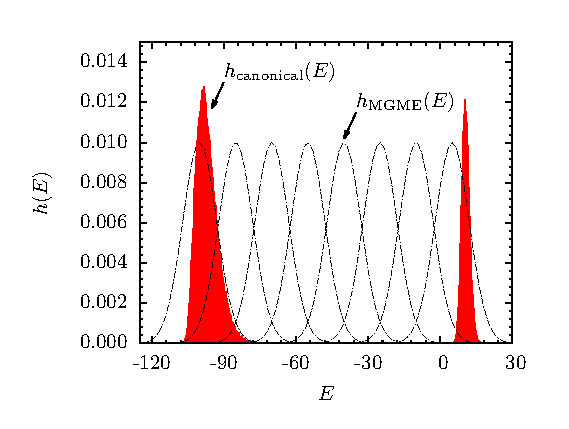
\includegraphics[width = 0.7\textwidth]{chapter3Figs/mgme.eps}
\caption{\label{fig:MGME}%
Canonical and GME energy histograms at a first-order pseudophase transition. The bimodal canonical energy histogram indicates the coexistence of ordered and disordered pseudophases, separated by an entropically suppressed energy region. Each GME ensemble enhances the sampling of suppressed states over a limited energy range.}
\end{figure} 
% 


Strong first-order transitions with bimodal energy distributions typically
require several overlapping GME ensembles to cover the relevant energy range, as illustrated in Fig.~\ref{fig:MGME}. The acceptance probability for the
exchange of conformations $(\mu,\nu)$ between neighboring GME ensembles with mean energies $(E_{G,i}, E_{G,j})$ at a constant inverse temperature $\beta$ is
%
\begin{equation}
a\left(\mu \leftrightarrow \nu \right) = 	
\mathrm{min}\left(1,e^{\Delta G}\right),
\end{equation}
%
where
\begin{equation}
\Delta G  = 
\frac{\left(E_{\mu} - E_{G,j}\right)^{2}-\left(E_{\nu}-
E_{G,j}\right)^{2}}{\Delta E_{G,j}^{2}} - \frac{\left(E_{\nu} - 	
E_{G,i}\right)^{2}-\left(E_{\mu} - E_{G,i}\right)^{2}}{\Delta E_{G,i}^{2}}.
\end{equation}

The direct product of GME ensembles defines the multiple Gaussian modified ensemble (MGME). With a proper choice of ensemble parameters $(E_{G},\Delta E_{G})$ it is possible to achieve a significantly enhanced sampling of previously inaccessible states. This can be further improved by allowing for exchanges between GME ensembles at different temperatures. However, previous knowledge of the system under consideration is usually needed to make a reasonable estimate for the ensemble parameters. Therefore other more systematic methods, such as the multicanonical \cite{muca1a,muca1b,muca2,muca3,muca4,Bachmann2013} and Wang-Landau sampling \cite{wl1,wl2,wl3}, are often used.    


\section{Histogram reweighting methods}

In chapter \ref{chap:elements_of_stat_mech}, we have introduced the microcanonical inflection point analysis as the means for the systematic study of pseudophase transitions in the microcanonical ensemble. Application of this method however presumes the precise knowledge of the microcanonical density of states $g(E)$ [Eq \ref{eq:densitOfStatesExplicit}]. Previously introduced sampling methods do not directly measure $g(E)$ but rather generate canonical energy histograms $h(E,\beta_{i})$. Hence, it is necessary to introduce a general method for estimating the density of states from energy histograms.

\subsection{Multiple\,-histogram reweighting}
Canonical histogram $h(E,\beta_{i})$ provides an approximation for the Boltzmann distribution $p_{\mathrm{can}}(E, \beta_{i})$, which is itself proportional to the microcanonical density of states
%
\begin{equation}
\label{eq:canonicalDistribution}
h(E,\beta_{i}) \approx p_{\mathrm{can}}(E, \beta_{i}) \propto g(E)e^{-\beta_{i}E}
\end{equation}
%
Therefore each histogram yields an estimate of the density of states 
%
\begin{equation}
\label{eq:singleHistogramReweighting}
\bar{g}_{i}(E) = h(E,\beta_{i})e^{\beta _{i} E}
\end{equation}
%
%
\begin{figure}
\center
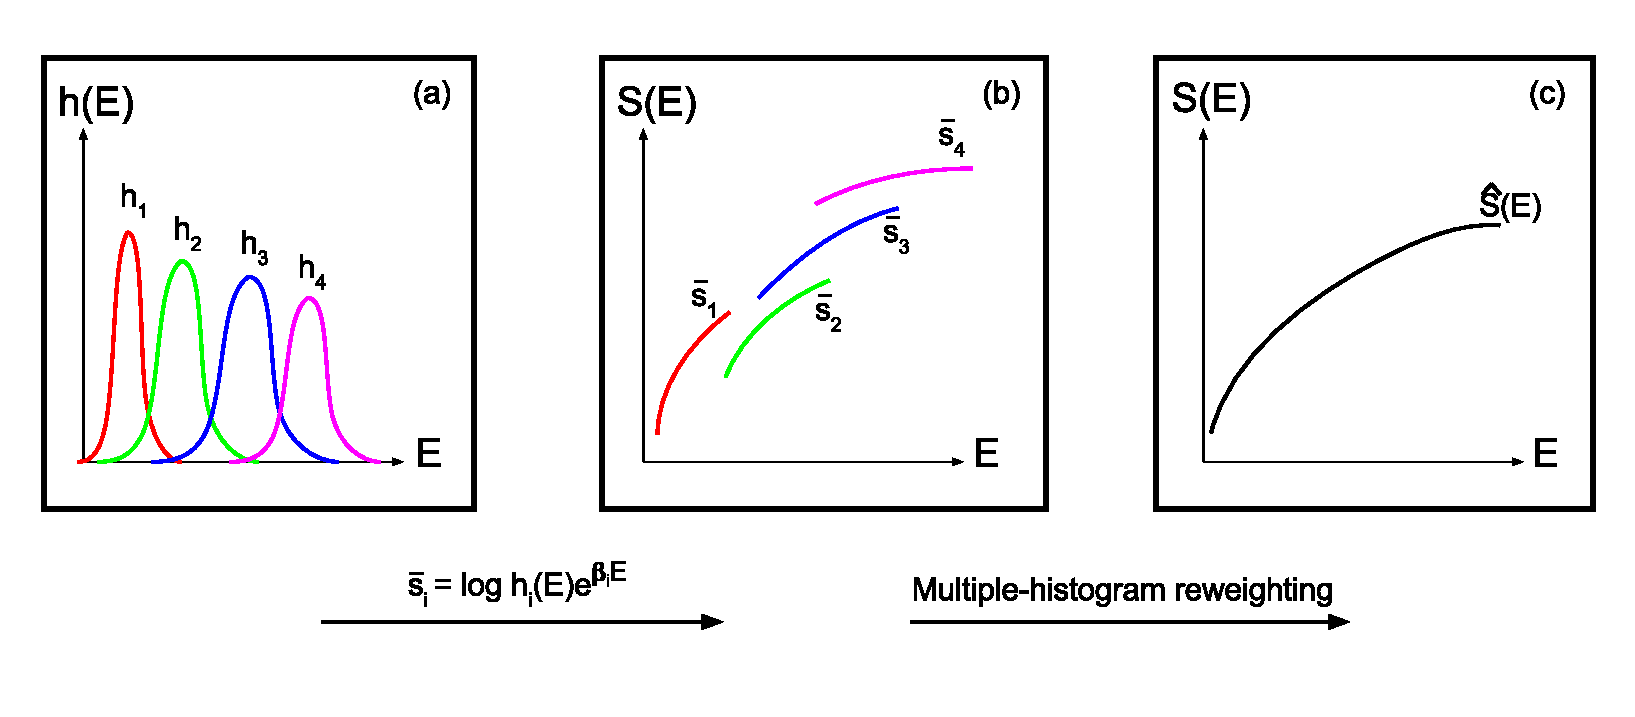
\includegraphics[width = 0.95\textwidth]{chapter3Figs/multipleHistogramReweighting.eps}
\caption{\label{fig:MHR}%
(a) Illustration of the canonical energy histograms $h(E,\beta_{i})$, (b) the individual estimates of the logarithm of the density of states $\bar{S}_{i}(E)$, (c) and the combined estimate of the logarithm of the density of states $\hat{S}(E)$ obtained by reweighting.}
\end{figure}
% 
Individual estimates $\bar{g}_{i}(E)$ are only reliable for energies in the
vicinity of the peak of the canonical histogram obtained at the temperature
$\beta _{i}$. Therefore a sufficient overlap between the histograms of
adjacent replicas is necessary to ensure that an accurate estimate of the density of states can be obtained for the entire energetic range. 

The task is now to combine the individual estimates $\bar{g}_{i}(E)$ and obtain an improved estimate $\hat{g}(E)$. Unfortunately, general Monte Carlo methods do not yield absolute estimates for the partition function $Z(\beta)$ and the estimates $\bar{g}_{i}(E)$ cannot be directly related if obtained at different temperatures.
However, it is possible to introduce a reference partition function
%
\begin{equation}
\label{eq:referencePartitionFunction}
\hat{Z}_i = \sum_E \hat{g}(E) e^{-\beta_i E},
\end{equation}
%
which serves as the appropriate weight in the estimator for the density of states
\begin{equation}
\label{eq:dosEstimator}
\hat{g}(E)= \frac{\sum_{i=1}^{R} h(E,\beta _{i})}{\sum_{i=1}^{R} M_i
\hat{Z}_i^{-1} e^{-\beta_i E}}.
\end{equation}
%
The equations \ref{eq:referencePartitionFunction} and \ref{eq:dosEstimator} must be solved iteratively until $\hat{g}(E)$ has converged. The relationship between the energy histograms, the individual estimates $\bar{g}_{i}(E)$, and the final estimate $\hat{g}(E)$ of the density of states is illustrated in Fig. \ref{fig:MHR}. For  detailed derivation and a further discussion of the multiple-histogram reweighting method please refer to \cite{Ferrenberg1989,Kumar1992}.

\subsection{Beziere smoothing}
The estimator for the density of states, obtained either by multiple-histogram reweighting or directly by multicanonical sampling, is not a smooth function but rather a discrete set of stochastic values. The formalism of the microcanonical inflection point analysis requires the accurate knowledge of its energy derivatives. These have to be computed by numerical differentiation which is prone to enhancing the random statistical fluctuations of the original data set. It is therefore desirable to approximate the density of states by a smooth analytic function, which can be done very effectively with Bezi\'{e}r curves \cite{Bachmann2014, Bezier1968}.

Bezi\'{e}r curve of order $n$ is a parametric curve defined by a set of $(n+1)$ control points $\left\lbrace P_{0},P_{1},....,P_{n}\right\rbrace$ and the formula 
%
\begin{equation}
\label{eq:beziereDefinition}
B(t) = \sum_{i=0}^{n}\mathcal{B}_{i}^{(n)}(t)P_{i},
\end{equation}
%
where ${B}_{i}^{(n)}$ are the Bernstein basis polynomials \cite{Lorentz1953} of degree $n$
%
\begin{equation}
\label{eq:BernsteinPoly}
{B}_{i}^{(n)}(t) = \binom{n}{i}(1-t)^{n-i}t^{i}.
\end{equation}
The discrete values of the estimated density of states $g(E_{i})$ serve as control points for the approximating Bezi\'{e}r curve. Assuming that the set of $(n+1)$ control points
\newline
$\left\lbrace g(E_{0}),g(E_{1}),....,g(E_{n})\right\rbrace$ is equally spaced in the energy space over the interval $[E_{\mathrm{min}},E_{\mathrm{max}}]$, the approximating Bezi\'{e}r function can be directly calculated from
%
\begin{equation}
g_{\mathrm{bez}}(E) = \sum_{i=0}^{n} \binom{n}{i} \left(\frac{E_{\mathrm{max}} - E}{E_{\mathrm{max}} - E_{\mathrm{min}}} \right)^{n-i} \left(\frac{E - E_{\mathrm{min}}}{E_{\mathrm{max}} - E_{\mathrm{min}}} \right)^{i} 
g(E_{i}).
\end{equation}
%
The numerical error introduced by the approximation scheme is typically much smaller than the random statistical fluctuations in the original noisy data set \cite{Bachmann2014}. However it should be mentioned that Bezi\'{e}r smoothing may introduce systematic errors to the derivatives of $g(E)$ in areas of abrupt changes in curvature.  This is illustrated in Fig. \ref{fig:Bezier} where we compare the noisy derivative of the microcanonical inverse temperature $\gamma(E) = d\beta/dE$ and the Bezi\'{e}r approximation $\gamma_{\mathrm{bez}}(E)$ in the region of a first-order pseudophase transition.
%
\begin{figure}
\center
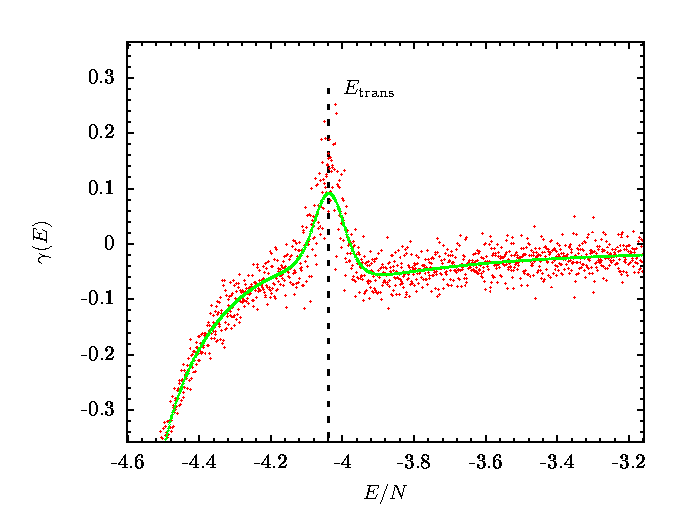
\includegraphics[width = 0.7\textwidth]{chapter3Figs/bezierComparison.eps}
\caption{\label{fig:Bezier}%
Comparison between the noisy derivative of the microcanonical inverse temperature $\gamma(E) = d\beta/dE$ and the Bezi\'{e}r approximation $\gamma_{\mathrm{bez}}(E)$. The systematic error in the Bezi\'{e}r approximation is visible near $E_{\mathrm{trans}}$, where the curvature of $\gamma(E)$ changes abruptly.
}
\end{figure}
% 
\section{Simple Monte Carlo updates}
The efficiency of Monte Carlo simulations depends in equal measure on the choice of  the sampling algorithm and on the selection of appropriate conformational updates. All update sets must be ergodic, i.e., it must be in principle possible to connect any two arbitrary states through a finite number of updates. Additionally, all updates must preserve the constraints of the model, such as volume exclusion and boundary conditions. The efficiency of individual updates depends strongly on the model to which they are being applied. Hence, there is no general set of updates that guarantees good performance across different physical models. In the following, we shall briefly discuss conformational updates which are suitable for simulations of off-lattice polymers and proteins. 

\subsection{Single displacement update}
The single displacement update is easy to implement, satisfies ergodicity, and has equal forward and backward selection probabilities. The original conformation of a polymer chain $\mathbf{R} = \{\mathbf{r_{1}},\mathbf{r_{2}},...,\mathbf{r_{N}}\}$ is updated by a random\footnote{Monte Carlo simulations make extensive use of pseudo-random numbers. The popular Mersenne Twister pseudo-random number generator \cite{Matsumoto1998} is used throughout this thesis. For more information on the `art' of random number generation please refer to \cite{Landau2000}.} displacement $\Delta \mathbf{r_{i}}$ of a randomly selected i-th monomer. The displacement vector is defined in the Cartesian coordinates as $\Delta \mathbf{r_{i}} = (\Delta x_{i}, \Delta y_{i}, \Delta z_{i})$, where each component is selected with uniform probability from some interval $[-l,\,l\,\,]$. In general, longer displacement updates lead to larger energy differences between the old and the new states $\Delta E = E_{\mathrm{new}} - E_{\mathrm{old}}$. In Monte Carlo simulations, large positive values of the ratio $\Delta E/T$ result in an exponential suppression of the acceptance rates [Eq. \ref{eq:MetropolisCriterionCanonical}]. In order to achieve acceptance rates within the optimal range of $\sim 30\%-70\%$, the set of temperature dependent displacement parameters $l(T_{i})$ must be determined. Unfortunately, for most off-lattice polymer models, only very short displacement updates are allowed at low temperatures and the generated sequence of states becomes strongly correlated. An example of the temperature dependence of $l(T_{i})$, obtained from a simulation of a flexible elastic 55-mer, is shown in Fig.\,\ref{fig:acceptanceRates}. Polymer models which contain stiff bonds cannot be sampled using displacement updates and require more sophisticated rotational updates \cite{Bachmann2014}.
%
\begin{figure}
\center
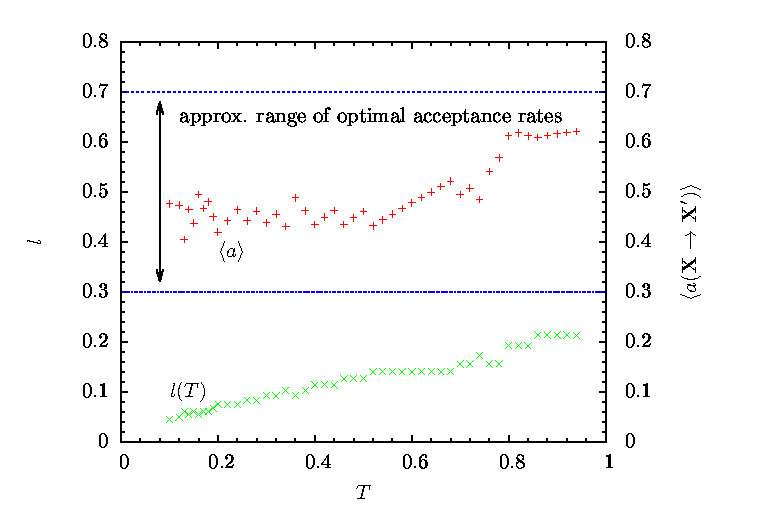
\includegraphics[width = 0.75\textwidth]{chapter3Figs/acceptanceRates.eps}
\caption{\label{fig:acceptanceRates}%
Example of a distribution of the temperature dependent displacement parameter $l(T)$, used in a parallel tempering simulation of a flexible elastic 55-mer. The values of $l(T)$ were selected to keep the average acceptance rates $\left\langle a \right\rangle$ within the optimal range of $\sim 30\%-70\%$.
}
\end{figure}
% 
\subsection{Pivot update}
The pivot update consists of rotating a portion of the polymer chain over a randomly chosen rotation axis. This allows for a global change in the polymer conformation and decreases the correlation between the sampled states. In practice, first a random monomer is selected to serve as the pivot and the direction of the rotation axis is defined by a random vector $\mathbf{k}$. With equal probability, either terminus of the chain is selected for rotation. The vector which connects the pivot to any monomer which is to be rotated is denoted as $\mathbf{r}$. The random rotation angle $\Delta \phi$ is selected with uniform probability from some interval $[-\lambda,\,\lambda]$. Finally, the projection $\mathbf{r}_{\bot}$ of the vector $\mathbf{r}$ into the plane perpendicular to $\mathbf{k}$ is rotated by $\Delta \phi$ and the resultant vector connecting the pivot and the rotated monomer is given by $\mathbf{r}^{\prime}$. A schematic depiction of the single-displacement and the pivot updates is provided in Fig. \ref{fig:conformUpdate}. It should be mentioned, that when used in simulations of polymer models with elastic bonds, the pivot update is not ergodic since it preserves bond length \cite{Bachmann2014}. Therefore it is recommended to combine rotational updates with single displacement updates whenever applicable. 

%
\begin{figure}
\center
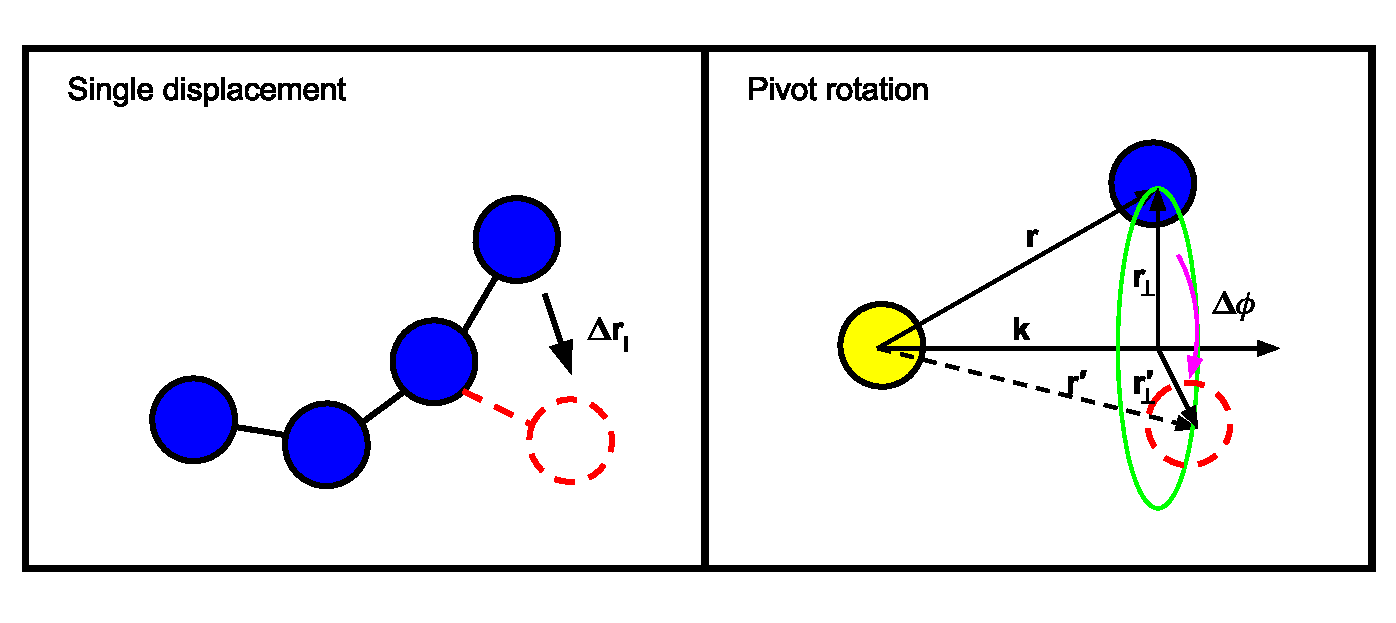
\includegraphics[width = 0.99\textwidth]{chapter3Figs/conformationalUpdates.eps}
\caption{\label{fig:conformUpdate}%
Schematic depiction of the single-displacement and the rotational pivot updates.
In a displacement update, a randomly selected monomer is moved according to a randomly generated displacement vector $\Delta \mathbf{r_{i}}$. The pivot update consists of rotating a portion of the polymer chain over a randomly chosen axis $\mathbf{k}$ by a random angle $\Delta \phi$. 
}
\end{figure}
% 


%%%%%%%%%%%%%%%%%%%%%%%%%%%%%%%%%%%%%%%%%%%%%%%%%%%%%%%%%%%%%%%%%%%%%%%%%%%%%%%%%%%%
%%%%%%%%%%%%%%%%%% 			CHAPTER 4     		%%%%%%%%%%%%%%%%%%%%%%%%%%%%%%%%%%%
%%%%%%%%%%%%%%%%%%%%%%%%%%%%%%%%%%%%%%%%%%%%%%%%%%%%%%%%%%%%%%%%%%%%%%%%%%%%%%%%%%%%



\chapter{Off-Lattice Polymer Models}
\label{chap:HomopolymerModel}
It is hardly possible to overestimate the importance of defining an appropriate model to represent a real physical system in a computational study. What constitutes an `appropriate' model depends largely on the system under investigation and on the level of detail which is needed to correctly capture the properties of a given physical phenomena. For example, the study of chemical reaction kinetics, ground-state geometries of molecules, or the optical and electronic properties of semiconductors, requires detailed knowledge of the electronic structure and interactions. In such cases, Density functional theory (DFT)\cite{Sholl2009} or other quantum mechanical modelling methods need to be employed. On the other hand, a wide range of interesting physical phenomena, such as protein folding, polymer collapse, adsorption, and aggregation, are driven by cooperative structure forming processes and as such are not expected to depend sensitively on the precise electronic or even atomic structures. In principle, it is possible to gain insight into these processes by the means of simplified models with a reduced number of effective parameters\cite{Bachmann2014,Schmid2011}. In this chapter we shall briefly discuss the concept of \textit{coarse-graining} and introduce the model for the flexible elastic homopolymer together with a set of structural order parameters which are particularly effective at characterizing the conformational geometries of polymers in the solid pseudophase.


\section{Coarse-grained models}
%
\begin{figure}
\center
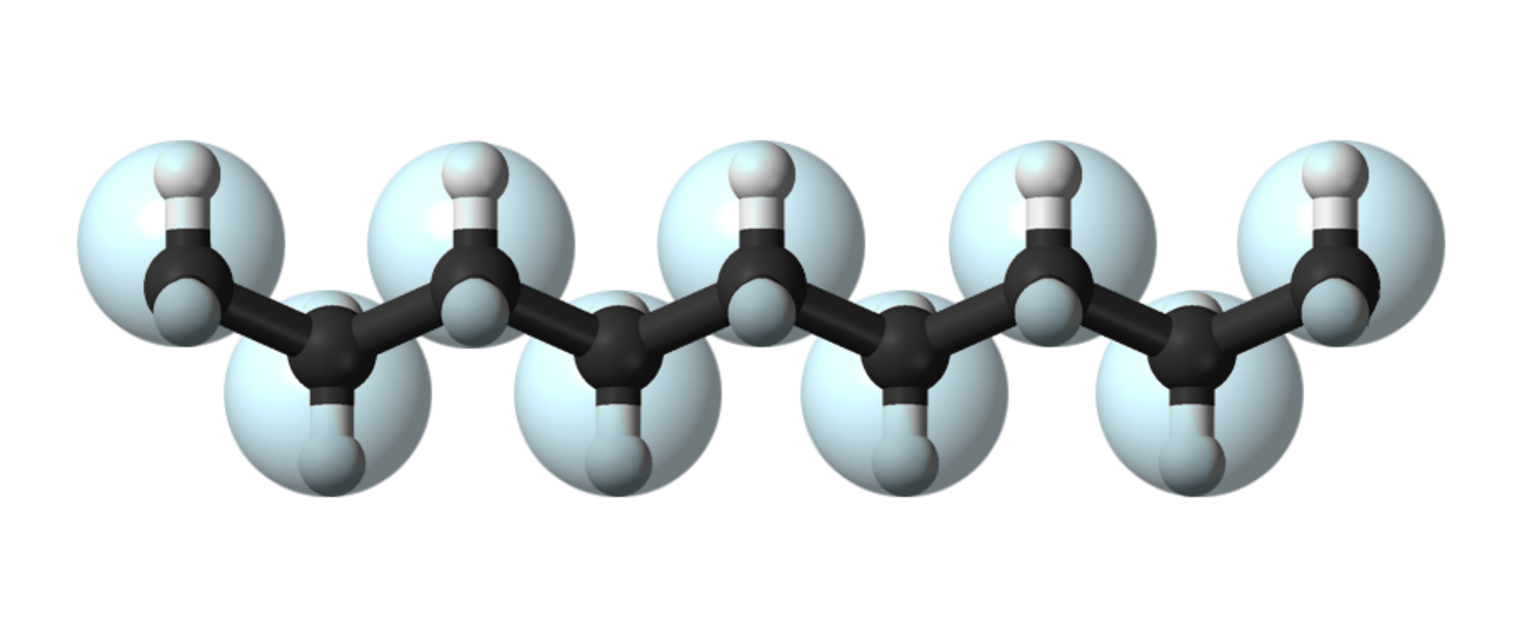
\includegraphics[width = 1.01\textwidth]{chapter4Figs/coarseGraining.eps}
\caption{\label{fig:coarseGraining}%
An example of a coarse-grained model of polyethylene. Methylene groups $(\mathrm{CH}_{2})$ are replaced by coarse-grained interaction sites which are depicted as transparent spheres. The interactions between the sites are described in terms of effective potentials.
}
\end{figure}
% 
The general idea behind \text{coarse-graining} is the observation that for a wide range of physical phenomena the individual degrees of freedom of a system do not act independently but rather behave in a cooperative fashion. The goal is then to find the minimal set of degrees of freedom which would allow for an accurate description of a given physical process. In the context of biomolecules, this typically amounts to replacing individual atoms by coarse-grained interaction sites and exact quantum many-body interactions by effective potentials [Fig. \ref{fig:coarseGraining}]. The new interaction sites are often referred to as \textit{monomers}. 


Individual conformations of a coarse-grained model with $N$ monomers can be represented by a $3N$-dimensional vector $\mathbf{Q} = (q_{1},q_{2},....,q_{3N})$ in the reduced coordinate system. The components $q_{i}$ represent the relevant degrees of freedom and are defined in terms of the map 
%
\begin{equation}
\tilde{q_{i}}(\textbf{X}): \textbf{X} \rightarrow \textbf{Q} 
\end{equation}
%
between the full conformational space $\mathbf{X}$ and the reduced space $\mathbf{Q}$. In the full conformational space, the canonical partition function is defined as
%
\begin{equation}
Z_{\mathrm{can}} = \int \mathcal{DX}e^{-\beta V(\mathbf{X})},
\end{equation}
%
where $V(\mathbf{X})$ is the exact inter-atomic potential. In order to express $Z_{\mathrm{can}}$ in terms of the coarse-grained coordinates, we begin by integrating out the microscopic degrees of freedom
%
\begin{equation}
Z_{\mathrm{can}} = \int \mathcal{DQ}\int \mathcal{DX}\prod _{i = 1}^{3N} \left[\delta (q_{i} - \tilde{q_{i}}(\mathbf{X}))\right]e^{-\beta V(\mathbf{X})}.
\end{equation}
Next we replace $V(\mathbf{X})$ by an effective potential
%
\begin{equation}
\label{eq:EffectivePotential}
\tilde{V}(\mathbf{Q}) = -k_{\mathrm{B}}\,T\,\mathrm{ln} \int \mathcal{DX}\prod_{i = 1}^{3N} \left[\delta (q_{i} - \tilde{q_{i}}(\mathbf{X}))\right]e^{-\beta V(\mathbf{X})}.
\end{equation}
%
and write
%
\begin{equation}
Z_{\mathrm{can}} = \int \mathcal{DQ}e^{-\beta \tilde{V}(\mathbf{Q})}.
\end{equation}
%
In principle, $\tilde{V}(\mathbf{X})$ contains the combined effects of the exact inter-atomic potentials and hence should allow for an accurate description of the thermodynamic and structural properties of the original system. However in reality, effective potentials are often only crude approximations to the definition introduced in Eq. \ref{eq:EffectivePotential}. The perhaps surprising fact, that a wide range of physical phenomena can be studied by the means of drastically simplified models, suggests that physical properties that arise through cooperative behaviors do not depend sensitively on microscopic details.

\newpage

\section{Flexible elastic homopolymer}
The generic model of a flexible, elastic, homopolymer is suitable for the investigation of the thermodynamic properties of polymer chains on a coarse-grained level. The polymer is represented by a linear chain of elastically bonded coarse-grained interaction sites, i.e., monomers [Fig.\,\,\ref{fig:singleChain}]. Individual monomers have neutral electric charges and do not interact via Coulomb forces. Instead, all structure forming processes are primarily driven by effective dipole-dipole interactions represented by the van Der Waals forces. 

The potential energy of a dipole-dipole interaction between a pair of monomers $(i,j)$ separated by the distance $r$ is given by 
\begin{equation}
V_{\mathrm{dip}}(r) = \frac{1}{4\pi \varepsilon _{0} }\frac{1}{r^{3}} \left[\mathbf{p}_{i}\cdot \mathbf{p}_{j} - 3\left(\mathbf{p}_{i}\cdot \hat{\mathbf{r}}\right)\left(\mathbf{p}_{j}\cdot \hat{\mathbf{r}}\right)\right],
\end{equation}
where $\mathbf{p}_{i}$ is the dipole moment of the $i$th monomer and $\hat{\mathbf{r}}$ is the unit vector in the direction given by the separation vector between the two monomers \cite{Griffiths1999}. However the strength of the potential decreases with the third power of the distance which is not consistent with the $1/r^{6}$ decay typically observed in experiments. In fact, the problem must be treated quantum mechanically to account for the existing overlap between electron wave functions. The potential $V_{\mathrm{dip}}(r)$ is replaced by a dipole-dipole operator $\hat{H}_{\mathrm{dip}}$, which is then introduced as a perturbation to a system of two non-interacting monomers. The first non-trivial term in the perturbation expansion of the ground state energy yields the desired $1/r^{6}$ dependence \cite{Bachmann2014}. In addition to this generic long range attraction, interacting bodies experience strong short range repulsion due to repelling electronic clouds. Both effects are contained in the famous Lennard-Jones potential \cite{Lennard-Jones1931}
%
\begin{equation}
U_{\mathrm{LJ}}(r_{ij})= 4\epsilon \left[ \left(
\frac{\sigma}{r_{ij}} \right)^{12} - 			\left(
\frac{\sigma}{r_{ij}} \right)^{6} \right], 
\label{eq:LJ1}
\end{equation}
%
where $\epsilon$  sets the energy scale of the interaction while the relevant length scale is given by the van der Walls distance $\sigma$ [Fig.\,\,\ref{fig:potentials}(a)].
 
%
\begin{figure}
\center
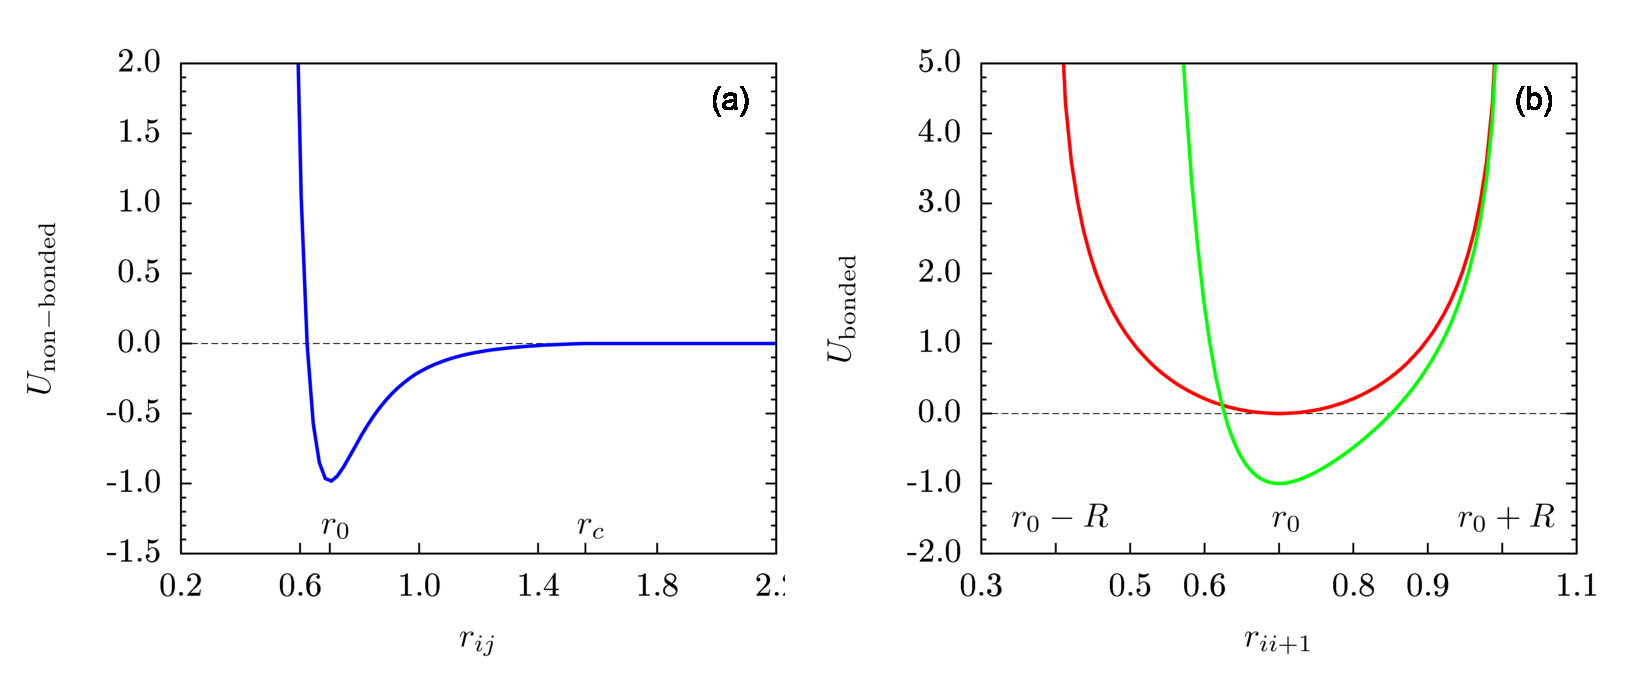
\includegraphics[width = 1.01\textwidth]{chapter4Figs/potentialLarge.eps}
\caption{\label{fig:potentials}%
(a) Non-bonded interactions in the generic model of an elastic homopolymer are represented by the Lennard-Jones potential. Interacting monomers experience strong repulsion below the equilibrium distance $r_{0}$, and are weakly attracted over the interval $(r_{0},r_{c})$ where $r_{c}$ marks the cutoff distance.\,\,(b) The nonlinear FENE potential (red) is a symmetric representation of the bonded interactions. As a possible variant, the symmetry of the bonded potential can be broken by combining the FENE and the Lennard-Jones potentials (green).}
\end{figure}
% 

The bonds between adjacent monomers are represented by an elastic potential which allows for longitudinal bond vibrations. The simplest approximation is given by the harmonic spring potential (Rouse model), however the linearity of the interaction force allows for large separation between the bonded monomers. This problem can be avoided by introducing a potential which diverges for $|r-r_{0}|\geq R$, where $r_0$ is the equilibrium bond length and $R$ controls the allowed fluctuation width. A particularly suitable choice is the finitely extensible nonlinear elastic (FENE) potential [Fig.\,\,\ref{fig:potentials}]\cite{Bird1987,Kremer1990,Milchev2001}
%
\begin{equation}
\label{eq:FENE}
U_{\mathrm{FENE}}(r_{ii+1})=-\frac{K}{2}R^2 
\mathrm{ln}\left[1-\left(\frac{r_{ii+1}-r_0}{R}\right)^2\right].
\end{equation}
%


\subsection{Single elastic chain}
\label{subsec:ElasticChain}
%
\begin{figure}
\center
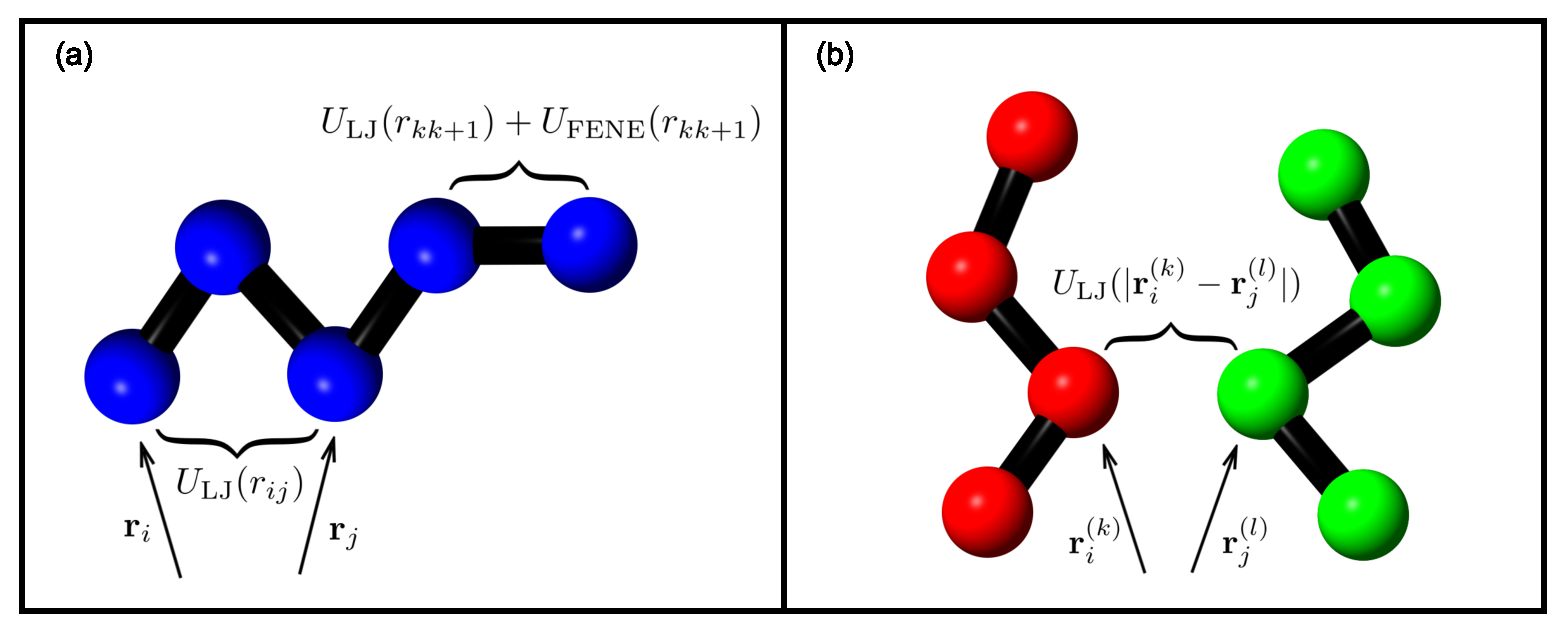
\includegraphics[width = 1.01\textwidth]{chapter4Figs/polymerModel.eps}
\caption{\label{fig:singleChain}%
(a) Generic model of a flexible elastic homopolymer. All monomers interact via a pairwise Lennard-Jones potential (LJ). Bonded interactions include an additional finitely extensible nonlinear elastic potential (FENE). (b) In a multi-chain system, the interactions between monomers belonging to different chains are also represented by the (LJ) potential.
}
\end{figure}
% 
In the following, we will define the model for a single elastic polymer chain which will be used for the remainder of this thesis [Fig.\,\,\ref{fig:singleChain}]. The specific values of the model parameters will be provided individually in the later chapters. The energy of a polymer chain of length $N$ in a conformation $\mathbf{X} = (\mathbf{r}_1,\cdots,\mathbf{r}_{N})$ is given by the sum of non-bonded and bonded contributions
\begin{equation}
E(\mathbf{X}) = \sum^{N}_{i<j+1}
U_{\mathrm{non-bonded}}(r_{ij}) + \sum^{N-1}_{i=1} 	
U_{\mathrm{bonded}}(r_{ii+1}). 
\label{totalE}
\end{equation}
%
 
All non-bonded interactions are represented by the Lennard-Jones potential introduced in Eq. \ref{eq:LJ1}. In order to reduce the number of required calculations in a computer simulation, it is a standard procedure to introduce a cutoff distance $r_{c}$ and set $U_{\mathrm{LJ}} = 0$ for all $r\geq r_{c}$. The truncated LJ potential must also be shifted vertically by the constant $U_{\mathrm{LJ}}(r_{c})$ to prevent a discontinuity at $r_{c}$. Hence the non-bonded interactions are represented by
%
\begin{equation}
\label{eq:LJTruncated}
U_{\mathrm{non-bonded}}(r_{ij}) = U_{\mathrm{LJ}}^{\mathrm{trunc}}(r_{ij}) =  \begin{cases}
U_{\mathrm{LJ}}(r_{ij}) -  U_{\mathrm{LJ}}(r_{c}), &
r_{ij} \leq r_{c},\\
0, &   r_{ij} > r_{c}. \end{cases}
\end{equation}
%
In addition to the FENE potential [Eq.\,\,\ref{eq:FENE}], bonded interactions contain an additional Lennard-Jones term
%
\begin{equation}
U_{\mathrm{bonded}}(r_{ii+1})= U_{\mathrm{FENE}}(r_{ii+1}) +  U_{\mathrm{LJ}}^{\mathrm{trunc}}(r_{ii+1}).
\end{equation}
%
The short range repulsive part of the LJ potential ensures that the resultant potential is asymmetric. The shapes of the bonded and non-bonded potentials are shown in Fig. \ref{fig:potentials}. 


\subsection{Interacting elastic chains}
A system of interacting elastic homopolymer chains is a suitable model for the study of generic features of macromolecular aggregation. The energy of $M$ interacting chains, each consisting of $N$ identical monomers, can be separated into intra-chain and inter-chain pairwise interactions
%
\begin{equation}
E_{\mathrm{total}} = E_{\mathrm{intra}} + E_{\mathrm{inter}}.
\end{equation}
%
The intra-chain contribution 
%%%%%% Intra-Chain Energy %%%%%%%
\begin{equation}
E_{\mathrm{intra}} = \sum^{M}_{k = 1}\sum^{N-1}_{i = 1}
U_{\mathrm{bonded}}(r\,^{(k)}_{ii+1}) +
\sum^{M}_{k=1}\sum^{N}_{i<j}
U_{\mathrm{non-bonded}}(r\,^{(k)}_{ij})
\end{equation}
%
consists of both bonded and non-bonded interactions, as defined in Sec.\,\,\ref{subsec:ElasticChain}, and $r\,^{(k)}_{ij}$ is the distance between the pair of monomers ($i$,$j$) of the $k$-th chain. The inter-chain contribution
%%%%%% Inter-Chain Energy %%%%%% 
\begin{equation}
E_{\mathrm{inter}} = \sum^{M}_{k < l}
\sum^{N}_{i,j}U_{\mathrm{LJ}}^{\mathrm{trunc}}(|\textbf{r}^{(k)}_{i}
- \textbf{r}^{(l)}_{j}|),
\end{equation}
%
consists solely of non-bonded Lennard-Jones interactions. Schematic depiction of the model is provided in Fig.\,\,\ref{fig:singleChain}\,\,(b).

\section{Structural order parameters}
\label{sec:orderParameters}
The formalism of the microcanonical inflection-point analysis, as introduced in section \ref{subsec: micro_analysis}, provides a systematic approach for the identification and classification of pseudophase transitions in mesoscopic systems. Further insight into the thermodynamic and structural properties of polymer systems can be obtained by identifying the set of conformations which are dominant in a given pseudophase. This can be accomplished either by visual inspection of sample structures, or more systematically, by introducing a suitable set of structural order parameters. 
%
\begin{figure}
\center
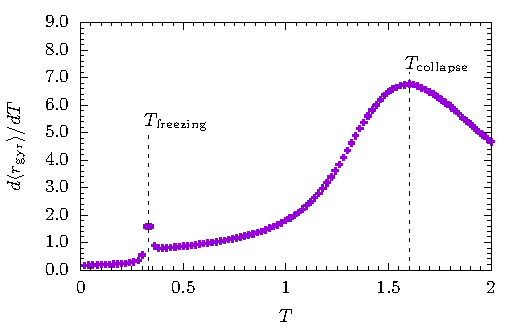
\includegraphics[width = 0.65\textwidth]{chapter4Figs/rogFluct.eps}
\caption{\label{fig:ROGFluct}%
The thermal fluctuations of the radius of gyration obtained from a Monte Carlo simulation of an elastic $55$mer. The distinct peaks indicate the locations of the freezing and collapse transitions at the temperatures $T_{\mathrm{freezing}}$ and $T_{\mathrm{collapse}}$ respectively.
}
\end{figure}
% 

An example of a useful and easily computable structural quantity is the radius of gyration
%
\begin{equation}
r_\mathrm{gyr}(\mathbf{X})=\sqrt{\frac{1}{N}\sum\limits_{i=1}^N
\left(\mathbf{r}_i-\mathbf{r}_\mathrm{com} \right)^2},
\end{equation}
%
where 
%
\begin{equation}
\mathbf{r}_\mathrm{com}=\frac{1}{N}\sum_{i=1}^N\mathbf{r}_i
\end{equation}
%
is the center-of-mass of the polymer conformation. The average $\langle r_{\mathrm{gyr}} \rangle$ is a measure of the compactness of the dominant conformations found at a given canonical temperature.
\newpage
\noindent
Signals, such as peaks and shoulders, in the temperature derivative 
%
\begin{equation}
\frac{d\langle r_{\mathrm{gyr}} \rangle}{dT} = \frac{\langle r_{\mathrm{gyr}} E \rangle - \langle r_{\mathrm{gyr}} \rangle \langle E \rangle }{k_{\mathrm{B}} T^{2}}
\end{equation} 
%
indicate locations of heightened thermodynamic activity and are routinely used to identify pseudophase transitions [Fig.\,\,\ref{fig:ROGFluct}].

Alternatively, a wide range of polymer conformation geometries can be identified using the set of rotationally invariant order parameters
%
\begin{equation}
Q_{l} = \left[ \frac{4\pi}{2l + 1} \displaystyle\sum_{m = -l}^{l}
|\rho_{l,m}|^{2} \right]^{1/2},	
\end{equation}
%
where 
\begin{equation}
\rho _{l,m} = \frac{1}{N}\sum _{i = 0} ^{N} \mathrm{Y}_{l,m}(\mathbf{r}_{i})
\label{eq:15}
\end{equation}
%
is the average of the real spherical harmonics\footnote{The real harmonics can be expressed in terms of the better known complex harmonics as
\begin{equation}
	\mathrm{Y}_{lm}(\mathbf{r}_{i}) =  \left\{
		\begin{array}{lr}
		\frac{i}{\sqrt{2}}\left[\mathrm{Y}_{l}^{m}(\mathbf{r}_{i}) -
(-1)^{m}\mathrm{Y}_{l}^{-m}(\mathbf{r}_{i})\right] & \quad \mathrm{if} \quad  m < 0,
\\[1.5ex]
		{Y}_{l}^{m}(\mathbf{r}_{i}) & \quad \mathrm{if} \quad  m = 0, \\[1.5ex]
		\frac{1}{\sqrt{2}}\left[\mathrm{Y}_{l}^{-m}(\mathbf{r}_{i}) +
(-1)^{m}\mathrm{Y}_{l}^{m}(\mathbf{r}_{i})\right] & \quad \mathrm{if} \quad  m > 0. \\
		\end{array}
	\right. 
\end{equation}
} evaluated at positions of the individual monomers \cite{Neirotti2000}. This set of order parameters has been particularly useful in the investigations of polymer systems exhibiting multiple solid pseudophases at low energies \cite{Koci2016}. In Fig.\,\,\ref{fig:orderParameters} we provide an illustration of this approach as applied to two different variants of a coarse-grained model of an elastic $15$mer. 


\begin{figure}
\center
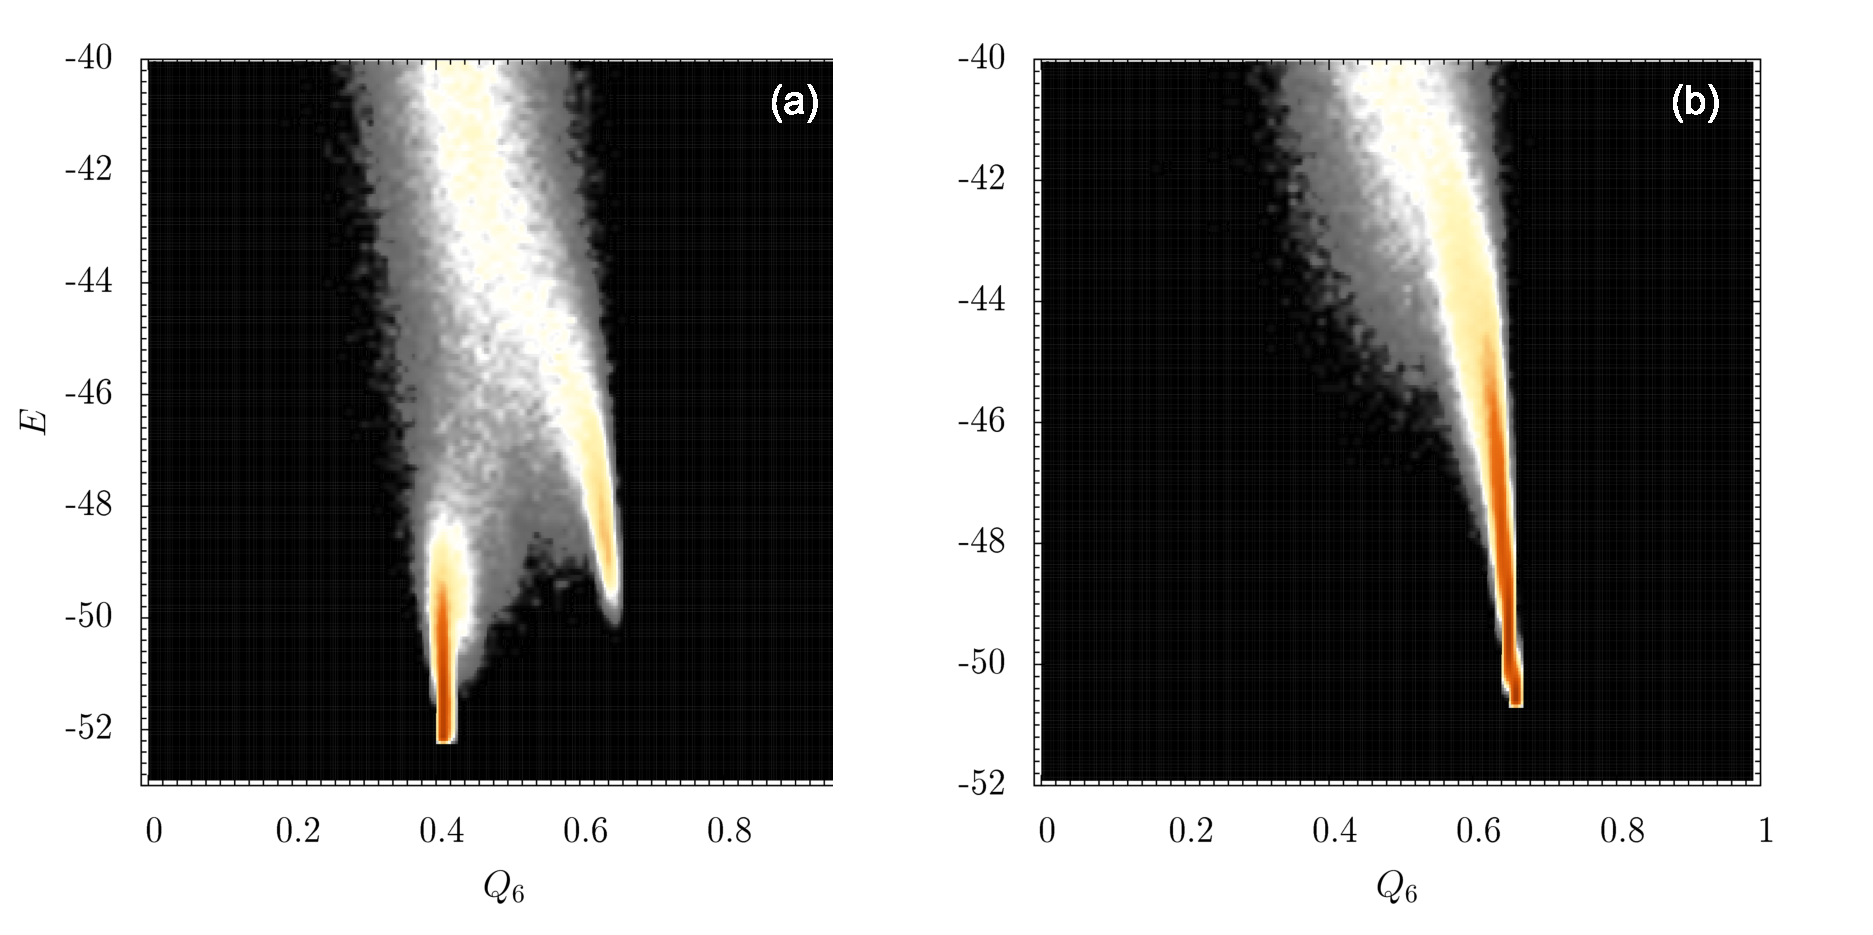
\includegraphics[width = 1.01\textwidth]{chapter4Figs/q6.eps}
\caption{\label{fig:orderParameters}%
Intensity plots of the rotationally invariant order parameter $Q_{6}$ for two variants of a coarse-grained model of an elastic $15$mer. The shading indicates the probability of detecting a configuration with a given value of the order parameter, red being the maximum probability and black being the lowest. In figure (a), the two prominent low energy branches reveal the existence of two solid pseudophases with distinct conformational geometries. Whereas in (b), only a single solid phase is detected.
}
\end{figure}
% 








%%%%%%%%%%%%%%%%%%%%%%%%%%%%%%%%%%%%%%%%%%%
%%%%%%%%%%%% CHAPTER 5 %%%%%%%%%%%%%%%%%%%%%%%%
%%%%%%%%%%%%%%%%%%%%%%%%%%%%%%%%%%%%%%%%%%%


\chapter{Impact of the Bond Confinement Range on the Structural Transitions of Elastic Homopolymers}
\label{chap:bondFluct}

In chapter \ref{chap:HomopolymerModel}, we have suggested that the structural and thermodynamic properties of polymer systems can be investigated by the means of rather simple coarse-grained models. It is desirable that the general features of the model, such as the types of observed pseudophases and low energy conformational geometries, remain at least qualitatively similar over a range of model parameters. In recent studies, the effect of the interaction range between non-bonded monomers of a single elastic homopolymer has been addressed systematically~\cite{taylorRange1,taylorRange2,Gross2013}. It has been found that for sufficiently short interaction ranges, it is possible for the polymer to fold directly from random-coil structures (i.e., the gas phase) into solid and compact conformations. Under these conditions, no globular (or liquid) phase is present.

In this chapter, we investigate the effects of restricting the fluctuation range of bonded interactions in a single elastic polymer chain. The variation of the bond extension range allows us to bridge the gap between self-interacting polymers with stiff bonds (such as proteins) and bead-spring chains (elastic polymers) with bonds so floppy that these polymers behave similarly to a gas of interacting particles. For this purpose, we have performed extensive replica-exchange Monte Carlo simulations in extended multiple Gaussian modified ensembles~\cite{Neuhaus2006}, which help improve the efficiency of parallel tempering simulations near first-order transitions. Systematic studies of the structural phases in the space of the bond confinement parameter were made possible by employing standard canonical analyses of fluctuations in macroscopic thermodynamic quantities and also by careful analysis of the nature of inflection points in the microcanonical temperature curve~\cite{Bachmann2014,Schnabel2011}.

\section{Model and simulation parameters}
In this study, we employ a coarse-grained model of an elastic homopolymer, in the same form as introduced in Sec.\,\,\ref{subsec:ElasticChain}. This model was originally introduced for investigations of general properties of elastic polymer chains. Due to the similarity in the transition behavior of atomic clusters and polymers, however, the scope of this model can be extended to investigate effects of bond confinement as well. As such, this model allows for the interpolation of systems ranging from polymers to an almost unconfined gas of atoms.

The energy and the length scales of the truncated and shifted Lennard-Jones potential (Eq.\,\,\ref{eq:LJTruncated}) were set to 
$\epsilon=1$ and $\sigma=r_0/2^{1/6}$ respectively, where $r_0 = 0.7$ marks the location of the minimum potential. The cut-off radius was set at $r_c=2.5\sigma$ such that $U_{\mathrm{LJ}}(r_{c}) \approx -0.0163169\epsilon$. The FENE potential (Eq.\,\,\ref{eq:FENE}), which together with the LJ potential represents bonded interactions, is used here in the modified form
%
\begin{equation}
\label{eq:ModFENE}
U_{\mathrm{FENE}}(r_{ii+1})=-\frac{K}{2}R_{0}^2 
\mathrm{ln}\left[1-\left(\frac{r_{ii+1}-r_0}{R}\right)^2\right], 
\end{equation}
%
%
\begin{figure}
\center
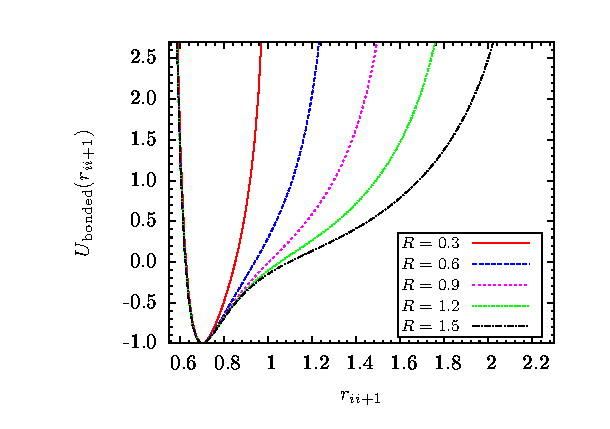
\includegraphics[width = 0.8\textwidth]{chapter5Figs/bond_potential.eps}
\caption{\label{fig:ModifiedBondedPotential}%
Behavior of the combined bond potential $U_{\mathrm{bonded}}(r_{ii+1}) = U_{\mathrm{LJ}}(r_{ii+1}) + U_{\mathrm{FENE}}(r_{ii+1})$ for different values of the effective bond confinement range $R$.}
\end{figure} 
%
where $K=40$ and $R_{0}=0.3$. The parameter $R$ inside of the logarithmic term controls the effective confinement range of the polymer bonds, whereas the energy scale of the potential is kept constant. The qualitative behavior of the combined bond potential for different values of $R$ is shown in Fig.~\ref{fig:ModifiedBondedPotential}. The bond elasticity increases with $R$, i.e., by changing $R$ in a wide range of values ($R\in[0.3,90]$), we systematically investigate an entire class of polymer systems between the limits of stiff polymers ($R\to 0$) and, effectively, a gas of nonbonded Lennard-Jones particles, for which $R\to \infty$.  

In our simulations, we have used the replica-exchange Monte Carlo\footnote{See also section\,\,\ref{subsec:ParallelTempering}} (parallel tempering)~\cite{sw1,geyer1,huku1,huku2}, extended to multiple Gaussian modified ensembles\footnote{See also section\,\,\ref{subsec:GaussianEnsemble}} (MGME)~\cite{Neuhaus2006}. The typical number of replicas in a simulation was $\sim80$, covering the temperature range $T\in [0.02,2.0]$. The total number of Monte Carlo sweeps per simulation totalled $5\times 10^8$. A replica exchange update was attempted every 100 Monte Carlo sweeps and accepted at an average rate exceeding 20\%. The acceptance rates for Metropolis updates in each thread was kept at $\sim 40-60\%$. Simulations were carried out on a two-dimensional mesh of temperatures and $E_G$ values in the first-order transition region. On average 10 different values of $E_G$ were used per temperature thread. The system was constrained inside of a steric sphere at a constant density of $0.001$ particles per unit volume, in which case the diameter of the sphere is larger than the length of the fully extended chain. Under these conditions, we consider the system to be highly dilute. 

The results presented in this chapter are compared for classes of polymers with $N=13$ and $30$ monomers. For verification purposes, we have also studied polymers with up to $55$ monomers, which, for this kind of systematic study that covers the entire parameter space, represents the limit of currently feasible simulations. 

\section{Results}
\label{sec:res}
%
In this section, we investigate the influence of the confinement parameter $R$ on the structural transitions in elastic chains of lengths $N = 13$ and $30$ in the dilute regime. For this purpose, we first perform a conventional canonical statistical analysis of fluctuating quantities and compare with results of a corresponding microcanonical analysis.
%
\subsection{Canonical analysis of energetic and structural fluctuations}
% 
For the identification of transition points, we first consider the changes in the thermodynamic behavior of energetic and structural canonical fluctuation quantities. The transition behavior is compared for various values of the confinement parameter $R$. This analysis enables us to construct a structural hyperphase diagram. Differences in the overall generic transition behavior are discussed for two system sizes ($N=13,30$). 

\newpage
 
The statistical fluctuation of a thermodynamic quantity $O$ is defined by the temperature derivative of its expectation value 
%
\begin{equation}
\langle O(\mathbf{X})\rangle(T)=\frac{1}{Z(T)}\int {\cal D}X\,
O(\mathbf{X}) e^{-E(\mathbf{X})/k_\mathrm{B}T},
\end{equation}
%
where ${\cal D}X$ is the integral measure in the space of all polymer conformations $\mathbf{X}$ and 
%
\begin{equation}
Z(T)=\int {\cal D}X\, e^{-E(\mathbf{X})/k_\mathrm{B}T}
\end{equation}
%
is the partition function of the canonical ensemble of these structures at the canonical (heat-bath) temperature $T$. Thus, changes in the monotonous behavior of 
%
\begin{eqnarray}
&&\hspace*{-7mm}\frac{d}{dT}\langle
O(\mathbf{X})\rangle(T)=\frac{1}{k_\mathrm{B}T^2}
\nonumber\\
&&\times
\left[\langle O(\mathbf{X})E(\mathbf{X})\rangle(T)-\langle
O(\mathbf{X})\rangle(T)\langle E(\mathbf{X})\rangle(T)\right]
\end{eqnarray}
%
indicate pronounced thermal activity of the system. The most common and easily accessible quantity in Monte Carlo simulations is the specific heat, which represents the fluctuations of energy\footnote{See also section\,\,\ref{sec:canonicalEnsemble}}. In this case $O=E$ and
%
\begin{equation}
c_V(T)=\frac{1}{N}\frac{d}{dT}\langle E(\mathbf{X})\rangle(T).
\end{equation}
%

The thermal fluctuations of the energy (specific heat) and of the radius of gyration\footnote{Radius of gyration was introduced in section\,\,\ref{sec:orderParameters}.} of 13mers and 30mers are shown in Fig.~\ref{fig:ElasPolyCanonicalResults}, for different values of bond confinement ranges $R$. Generally, peaks and ``shoulders'' in these quantities indicate locations of structural transitions. The generic transitions of elastic chains are the $\Theta$ collapse transition that separates the gas-like phase of random-coil conformations from the liquid, collapsed globular phase, and the freezing transition from the globular into the solid ``crystalline'' phase~\cite{svbj1,Schnabel2009}. Interestingly, previous studies have shown that both transitions merge if \emph{nonbonded} interactions are restricted to extremely short-ranges~\cite{taylorRange1,taylorRange2,Gross2013}. 
%
\begin{figure}
\center
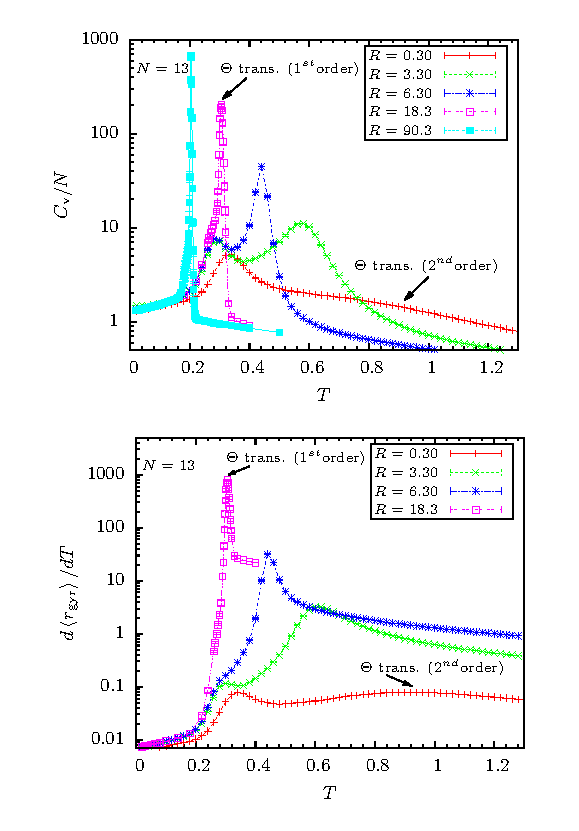
\includegraphics[width = 0.49\textwidth]{chapter5Figs/canon13.eps}
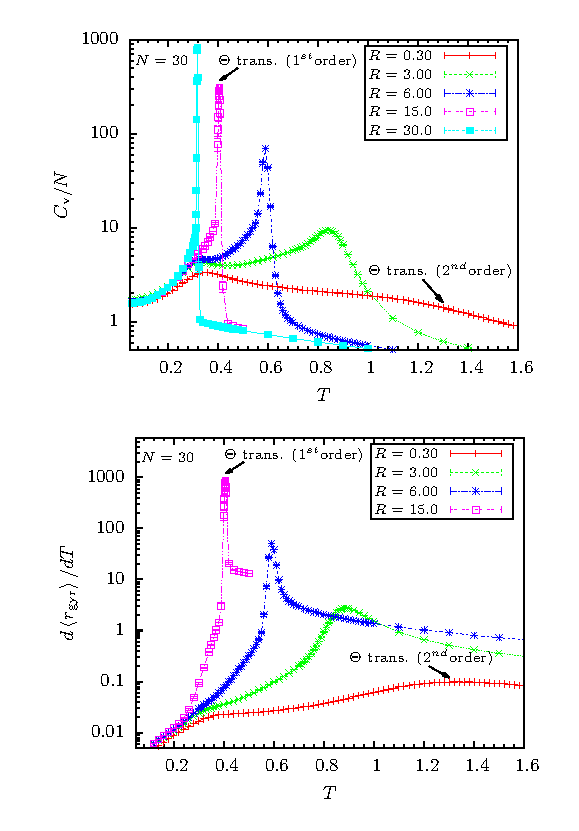
\includegraphics[width = 0.49\textwidth]{chapter5Figs/canon30.eps}
\caption{\label{fig:ElasPolyCanonicalResults}%
Specific heat and the thermal fluctuations of the radius of gyration for 13mers and 30mers, parametrized by the bond confinement parameter $R$.}
\end{figure} 
%
We have observed similar behavior in systems where extremely large bond fluctuations are allowed. Whereas, with increasing values of $R$, the low-temperature signal in the specific-heat curves in Fig.~\ref{fig:ElasPolyCanonicalResults} (which, for example, for $R=3.0$ is still clearly associated with the freezing transition) shifts only slightly to lower temperatures, the $\Theta$ transition signal drops significantly and finally merges with the freezing transition at $R\sim 30$. Whether the freezing and $\Theta$ transitions remain well separated for all values of $R < 30$ cannot be unambiguously determined by inspection of the canonical fluctuation quantities, in particular since for $R > 15$ the freezing transition signal turns into a shoulder on the low-temperature flank of the more dominant $\Theta$ transition peak. We will provide evidence for the separation of the transitions, using the methods of microcanonical analysis in the next section.

The general properties of the freezing transition do not change noticeably until its merger with the $\Theta$ transition. This is plausible since the freezing transitions
are driven mainly by the Lennard-Jones pair interactions between bonded and nonbonded monomers that optimize the icosahedral-like conformations in the solid phase. Therefore, this transition is not significantly affected by the modifications in the bond elasticity. 

In the solid phase, the ``magic'' 13mer possesses a perfect icosahedral shape~\cite{svbj1,Schnabel2009}, whereas the 30mer forms amorphous structures. The energy histograms of the 13mer exhibit bimodal shapes near the freezing transition point for values of $R <  30$, suggesting a first-order-like transition of the finite system. The ``liquid-solid'' transition of the 30mer resembles a ``liquid-liquid'' transition, since the compact globular conformations are difficult to distinguish from the amorphous solid structures. Nonetheless, the transition signal is clearly visible and the unimodal shape of the canonical energy histograms (not shown) in this region of $R$ space  indicates a second-order-like transition.

More striking is the dramatic change of the characteristic features of the $\Theta$ transition. As expected, for $R \sim 0.3$, the transition is still \emph{second-order-like}~\cite{Lifshitz1978,Khokhlov1981}. In the specific heat-curves in Fig.~\ref{fig:ElasPolyCanonicalResults} it is clearly visible that with increasing values of $R$, the shoulders indicating the $\Theta$ transitions turn into distinct peaks which rapidly become narrower and more pronounced as they shift to lower temperatures. For values of  $R > 4.5$, the canonical energy histograms obtained at the transition temperature are no longer unimodal, which suggests that the $\Theta$ transition become \emph{first-order-like}. This can be seen nicely in  Fig.~\ref{fig:ElasPolyhist13}, where energy histograms for the 13mer with $R=15$ at temperatures near the $\Theta$ transition point are shown. For temperatures near $T=0.33$, the bimodal shape of the histograms is clearly visible. The phase separation between gas and liquid is unusual for a polymer and indicates that for $R=15$ the particles in the system are quasi-free and behave rather like a loosely confined interacting gas, because bond-crossings are possible. The disappearance of the two distinct transition signals for $R > 30.0$ marks the end of existence of a separate liquid phase. This behavior is similar for both systems sizes studied and might be universal. However, the strikingly prominent signals for the $\Theta$ transition and the disappearance of the liquid phase are limited to the dilute regime and would not be observed at higher particle densities~\cite{frantz,frant2}. 
%
\begin{figure}
\center
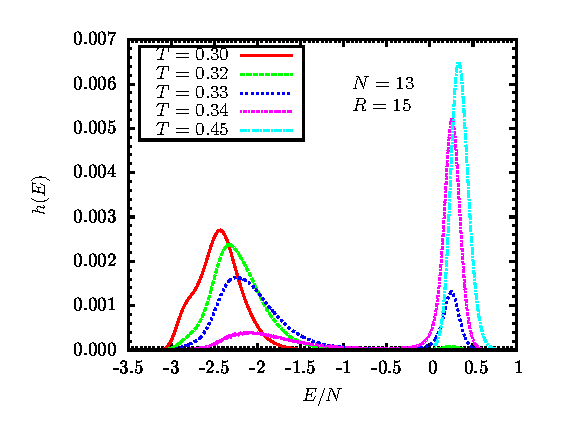
\includegraphics[width = 0.7\textwidth]{chapter5Figs/hist13.eps}
\caption{\label{fig:ElasPolyhist13}%
Energy histograms of the 13mer with $R=15$ at several temperatures near the $\Theta$ point. The bimodal shape of the histograms near the transition temperatur $T_{\theta } = 0.331$ clearly indicates a first order pseudophase transition.}
\end{figure}
%
It should be mentioned that the phase separation becomes substantially stronger for larger $R$ values, as well as the interfacial surface tension due to the radical entropic depletion in the energetic gap region.

With the transition temperatures obtained from the peaks in the canonical quantities we construct structural phase diagrams parametrized by the temperature $T$ and the confinement parameter $R$. For both system sizes, near the unmodified values of $R$, we observe three distinct structural phases. The high-temperature curves in Fig.~\ref{fig:ElasPolyPhaseDiagrams} represent the $\Theta$ transition lines, at which the expanded coils in the gas phase collapse into the compact but disordered globular states in the liquid phase. The green and red portions of the $\Theta$ transition line indicate the regions in which the transition is second-order-like and first-order-like respectively. The merging of the freezing and the $\Theta$ lines indicates the absence of the liquid phase and a direct transition from the gas to the crystalline phase for values of $R > 30$. The apparent similarities between the phase diagrams in the $\Theta$ regime suggest that similar behavior in systems of larger sizes could be expected. The different order of the liquid-solid transition (first order for the 13mer and second order for the 30mer) is a consequence of the entropic character of the solid phase. For the 13mer, the icosahedron is the all dominating morphology with comparatively low entropy and specific energy that sets apart the liquid phase and creates a phase-separation scenario. On the other hand, the ``solid'' phase of the 30mer is of rather highly entropic amorphous nature and allows for a continuous crossover from the liquid phase. 

%
\begin{figure}
\center
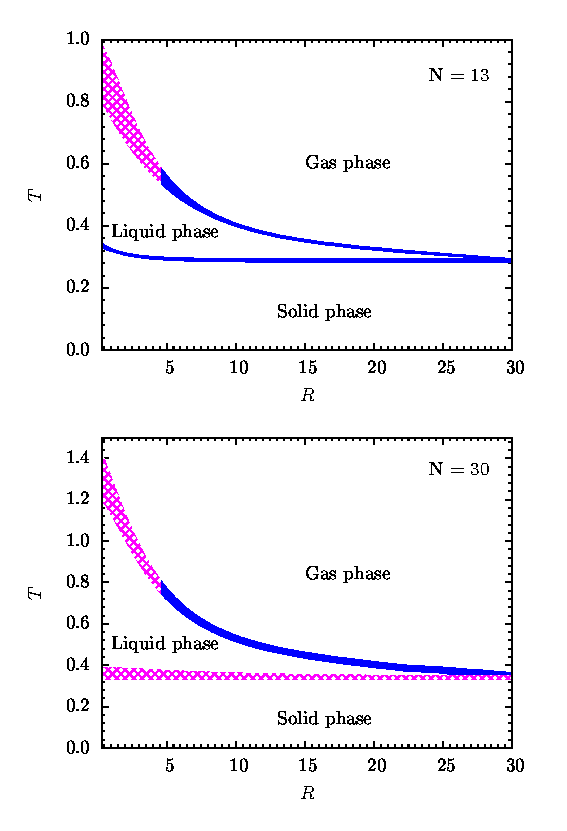
\includegraphics[width = 0.7\textwidth]{chapter5Figs/pd1330.eps}
\caption{\label{fig:ElasPolyPhaseDiagrams}% 
Structural phase diagrams for 13mers and 30mers, parametrized by the canonical temperature $T$ and the confinement parameter $R$. The blue (solid) and pink segments indicate first-order-like and second-order-like transitions, respectively.}
\end{figure}
%

It is instructive to consider the effects of the bond confinement range on ground state conformations. It was previously shown~\cite{Gross2013} that a decrease in the interaction range of the Lennard-Jones potential can lead to the disappearance of icosahedral ground-state structures in ``magic'' system sizes (such as $N=55$). In the present study, the ground state energies remained virtually constant and the conformations of 13mers retained their icosahedral geometry even for extremely high values of the parameter $R$. This suggests that the low-temperature behavior of flexible homopolymer chains is dominated by Lennard-Jones interactions while the FENE potential influences only the particular orderings of monomers within the ground-state structures.

\subsection{Results of microcanonical inflection-point analysis}
%
As discussed in the previous section, the results obtained by means of canonical analysis suggest that the $\Theta$ transition acquires first-order-like character in systems with large bond confinement range. However, the analysis of structural transitions based on canonical quantities is often ambiguous. Canonical energy histograms are useful for determining the order of a transition only if their shape is clearly bimodal or unimodal. In this section, we turn to microcanonical inflection-point analysis\footnote{See also section \ref{subsec: micro_analysis}} which offers a robust and unambiguous approach towards the classification of structural transitions~\cite{Bachmann2014,Bachmann2013,Schnabel2011}. 

In Fig.~\ref{fig:ElasPolyMicrocanonicalResults} we summarize the results for chains of lengths with $N = 13$ and $30$ monomers for values $R = 0.3, 4.5, 30.0$. In addition to the microcanonical temperature $\beta(E)$ and its first derivative $\gamma(E) = d\beta/dE$, we also plot the canonical energy histograms $h(E)$ obtained at the $\Theta$ transition temperature. 

%
\begin{figure}
\center
\hspace*{-5mm}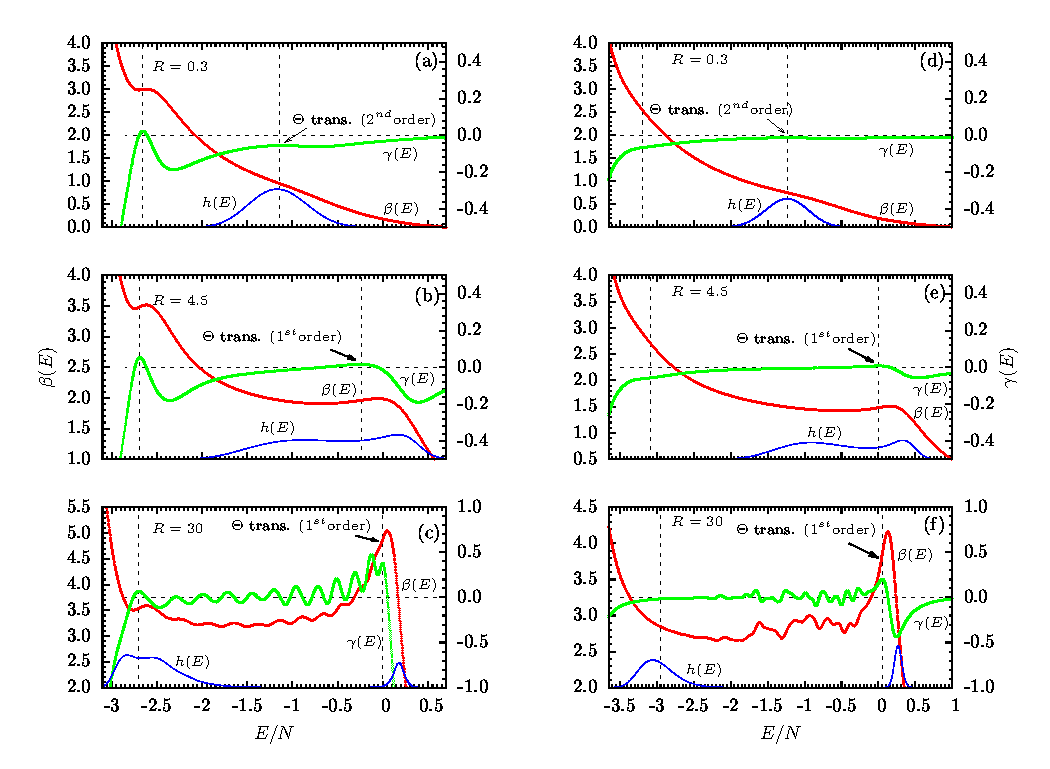
\includegraphics[width= 1.05\textwidth]{chapter5Figs/microelast.eps}
\vspace{5mm}
\caption{\label{fig:ElasPolyMicrocanonicalResults}%
Microcanonical results for 13mers with bond confinement ranges  (a) $R=0.3$, (b) $4.5$, and (c) $30$ as well as for 30mers (d)-(f). Shown are inverse temperature curves $\beta(E)$, their first derivatives $\gamma(E)=d\beta(E)/dE$, and (on arbitrary scale) the energy histograms $h(E)$ at the $\Theta$ transition temperature. The horizontal dashed line marks $\gamma=0$. The positive valued peaks of $\gamma (E)$ for values of $R > 4.5$ clearly indicate that the $\Theta$ transition is first order, but remains separate from the freezing transition. The absorption of the freezing transition by the $\Theta$ transition is apparent for large confinement ranges (c, f).}
\end{figure}
%

For $R = 0.3$, the negative valued peaks of $\gamma(E)$ indicate that the $\Theta$ transition is of second order, in agreement with the observation that the canonical energy histograms for both system sizes are clearly unimodal. At $R = 4.5$, the peaks of $\gamma(E)$ become positive and we conclude that the $\Theta$ transition turns to first order. The signals for freezing transitions remain well outside of the back-bending region of the $\Theta$ transition, confirming that the two transitions are well separated.

In the case $R = 30$, the multiple peaks in $\gamma(E)$ indicate that the $\Theta$ transition consists of a hierarchy of subphase transitions. This interesting phenomena is characteristic of nucleation transitions with entropy reduction due to stepwise loss of translational entropy. One prominent example is the aggregation transition in systems consisting of multiple polymer chains~\cite{Bachmann2014,KociAgg2015,Junghans2008,Junghans2009,Junghans2011},
which will be discussed in detail in Chap.\,\,\ref{chap:Aggregation}. Here, the system undergoes a direct transition from the solid phase into the gas phase through a series of subphase transitions consisting of individual monomers breaking away from the bulk.
\newpage
\noindent
This can be seen nicely in the case of a 13mer with the confinement range $R = 30$. Shown in Fig.~\ref{fig:ElasPolyMicrocanonicalResults}(c), each of the 12 oscillations in the back-bending region of $\beta(E)$ corresponds to a subphase transitions. For a 30mer, at the same $R$ value [Fig.~\ref{fig:ElasPolyMicrocanonicalResults}(f)], subphases overlap to an extent that only an accumulated effect upon $\beta(E)$ is visible. 

The freezing transition is no longer an autonomous transition but instead becomes one of the subphase transitions that make up the $\Theta$ transition. Eventually, this entails the absence of a separate liquid phase, which is in agreement with the overall picture obtained by the canonical analysis of fluctuating quantities.

The maximum $R$ value is, of course, limited by the boundary of the simulation sphere that represents a steric constraint. The presence and the stability of the individual structural phases depend on the particle density. In the scenario presented here, where we investigate the disappearance of the liquid phase, we fixed the density to $0.001$ particles per unit volume, whereas additional simulations at a $10$ times larger density showed that the liquid phase remained stable, even for bond confinement ranges as large as $R=100$. In the unconstrained case of open boundaries (which for fixed particle number means vanishing density) and $R\to\infty$, both liquid and solid phase are supposed to disappear and the gas phase would remain as the only stable phase. The disappearance of phases by reducing confinement has already been observed in atomic cluster systems some time ago~\cite{calvo1,calvo2}.

In Tables~\ref{tab:ElasPolyTab1} and~\ref{tab:ElasPolyTab2}, we have listed the transition temperatures $T_{\mathrm{f},\theta}$ and latent-heat values per monomer $\Delta q_{\mathrm{f},\theta}$ for 13mers and 30mers at various bond confinement ranges $R$. Transition temperatures for the second-order transitions were obtained by microcanonical inflections-point analysis, whereas the transition points and latent heat values were estimated by means of microcanonical Gibbs construction.\footnote{For a description of the microcanonical Gibbs construction please refer to section\,\,\ref{subsubsec:InflectionPointAnalysis}.}
%

%
\begin{table}
\caption{\label{tab:ElasPolyTab1}%
Microcanonical transition temperatures $T_{\mathrm{f},\theta}$ and latent heats $\Delta q_{\mathrm{f},\theta}$ at the freezing and $\Theta$ transition points, respectively, for 13mers with different bond confinement ranges $R$.}
\begin{tabular*}{\hsize}{@{\extracolsep{\fill}}rcccc@{}}
$R$& $T_{\mathrm{f}}$ & $T_{\theta}$ & $\Delta q_{\mathrm{f}}$ & $\Delta
q_{\mathrm{\theta}}$\\
\hline
$0.3$  &  $0.334 \pm 0.005$ &  $1.1 	\pm 0.1$ 	& $0.157 \pm 0.002$
& N/A\\
$1.5$  &  $0.306 \pm 0.005$ &  $0.9 	\pm 0.1$		& $0.090
\pm 0.002$ & N/A\\
$3.0$  &  $0.291 \pm 0.005$ &  $0.64	\pm 0.05$	& $0.208 \pm 0.002$
& N/A\\
$4.5$  &  $0.286 \pm 0.005$ &  $0.52	\pm 0.01$ 	& $0.228 \pm 0.002$
& $1.132 \pm 0.005$\\
$9.0$  &  $0.283 \pm 0.005$ &  $0.387	\pm 0.005$  	& $0.249 \pm 0.002$
& $2.133 \pm 0.002$ \\
$15.0$  &  $0.282 \pm 0.005$ &  $0.331  \pm 0.005$	& $0.254 \pm 0.002$
& $2.485 \pm 0.002$ \\
$30.0$  &  $0.282 \pm 0.005$ &  $0.284  \pm 0.005$ 	& $0.285 \pm 0.002$
& $2.978 \pm 0.002$ \\
\hline
\end{tabular*}
\end{table}
%
\begin{table}
\caption{\label{tab:ElasPolyTab2}%
Same as Table~\ref{tab:ElasPolyTab1}, but for 30mers.}
\begin{tabular*}{\hsize}{@{\extracolsep{\fill}}rcccc@{}}
$R$& $T_{\mathrm{f}}$ & $T_{\theta}$ & $\Delta q_{\mathrm{f}}$ & $\Delta
q_{\mathrm{\theta}}$\\
\hline
$0.3$  &  $0.39 \pm 0.01$ &  $1.3 	\pm 0.1$ 	& N/A & N/A\\
$1.5$  &  $0.39 \pm 0.01$ &  $1.2 	\pm 0.1$		& N/A &
N/A\\
$3.0$  &  $0.38 \pm 0.01$ &  $0.88	\pm 0.05$	& N/A & N/A\\
$4.5$  &  $0.37 \pm 0.01$ &  $0.69	\pm 0.01$ 	& N/A & $1.650 \pm
0.005$\\
$9.0$  &  $0.36 \pm 0.01$ &  $0.496	\pm 0.005$  	& N/A & $2.647 \pm
0.002$ \\
$15.0$  &  $0.35 \pm 0.01$ &  $0.416  \pm 0.005$	& N/A & $3.057 \pm
0.002$ \\
$30.0$  &  $0.35 \pm 0.01$ &  $0.344  \pm 0.005$ & N/A & $3.399 \pm 0.002$
\\
\hline
\end{tabular*}
\end{table}
%
\section{Summary}
\label{sec:sum}
%
In this chapter, we have investigated the thermodynamic behavior of a linear chain of monomers connected by confined bonds, which resembles a polymer for a large range of values of the bond confinement range $R$. Advanced parallel replica-exchange Monte Carlo methods, such as the Multiple Gaussian modified ensemble (MGME), were utilized in order to overcome the computational difficulties posed by the strong first-order-like behavior associated with the $\Theta$ transition at large $R$ values. Using the results obtained from the specific heat and the thermal fluctuations of the radius of gyration, we have constructed and compared features of the structural hyperphase diagrams for 13mers and 30mers. For low and intermediate confinement ranges, three distinct structural phases separated by the freezing and the $\Theta$ transitions can be identified, in agreement with the expected behavior. With increasing values of the parameter $R$, however, the $\Theta$ transition line shifts to lower temperatures and eventually merges with the freezing transition line, suggesting the absence of an independent liquid phase. Microcanonical inflection-point analysis provides conclusive evidence that the $\Theta$ transition turns from second order to first order if the bond confinement range parameter $R$ exceeds a threshold value. This change in the character of the $\Theta$ transition is not influenced by the freezing transition, which in this part of the phase diagram is still well separated from the $\Theta$ point. Increasing the confinement range further, $\Theta$ and freezing transitions merge and exhibit clear indications of a hierarchical nucleation transition. In this regime, the beads  are quasi-free and interact likewise with others, bonded or nonbonded. The still coupled system behaves like an atomic cluster in a dilute regime. The general structure of the hyperphase diagrams can be expected to remain qualitatively intact even for substantially larger systems. The only anticipated change is that the freezing transition is of first order for all system sizes with more than about 40 monomers~\cite{Schnabel2011}.

Our systematic study covers the technologically and biologically interesting regime of polymer chains with bond elasticities ranging from stiff to highly elastic, which includes all realistic linear macromolecules,  and extends into the space of confined systems that behave like atomic clusters. Since our results are supposed to be generic, they allow for a classification of the expected transition behavior on the basis of the effective bond confinement range of these systems.
%

%%%%%%%%%%%%%%%%%%%%%%%%%%%%%%%%%%%%%%%%%%%%%%%%%%%%%%%%%%%%%%% 	     
%%%%%%%%%%%%%%%%%%%%   CHAPTER 6			   %%%%%%%%%%%%%%%%%%%
%%%%%%%%%%%%%%%%%%%%%%%%%%%%%%%%%%%%%%%%%%%%%%%%%%%%%%%%%%%%%%%

\chapter{Effects of Short Range Repulsion on the Structural Properties of Elastic Homopolymers}

Bonded interactions in coarse-grained models of elastic polymers are commonly represented by the symmetric, finitely extensible nonlinear elastic (FENE) potential (Eq.~\ref{eq:FENE}). In Chap.~\ref{chap:HomopolymerModel}, we have introduced an alternative form of the bonded potential with an added Lennard-Jones (LJ) term. With the additional term, the bonded potential becomes strongly repulsive at close ranges, and the symmetry of the FENE potential is broken. However the maximum extension of the bond, also known as the bond confinement range, is controlled solely by the strongly diverging FENE potential.  The impact of the bond confinement range on the thermodynamic properties of short elastic homopolymer chains is discussed extensively in Chap.~\ref{chap:bondFluct}. In the following, we systematically investigate the effects of short range repulsion between bonded monomers on the structural properties of polymer chains of length $N = 15,55$. 
\newpage
\noindent
Structural phase diagrams are constructed utilizing the methods of canonical and microcanonical analysis. The geometry of low energy conformations is examined with the aid of structural order parameters which were introduced in Sec.~\ref{sec:orderParameters}.

%%%%%%%%%%%%%%%%%%%%%%%%%%%%%%%%%%%%%%%%%%%%%%%%%%%%%%%%%%%%%%% 	     
%%%%%%%%%%%%%%%%%%%%  MODEL AND METHODS		 %%%%%%%%%%%%%%%%%
%%%%%%%%%%%%%%%%%%%%%%%%%%%%%%%%%%%%%%%%%%%%%%%%%%%%%%%%%%%%%%%
\section{Model and Simulation Parameters}
In this study, we simulate the coarse-grained model of an elastic homopolymer, which has already been introduced in Chap.~\ref{chap:HomopolymerModel}. The energy scale of the Lennard-Jones potential is set to $\epsilon=1$ and the van-der-Waals radius to $\sigma=r_0/2^{1/6}$, where $r_0 = 1.0$ is the location of the potential minimum. We set a cut-off radius at $r_c=2.5\,\sigma$ and introduce a shift $U_{\mathrm{LJ}}(r_{c}) \approx -0.0163169$, to avoid discontinuities in the potential.

In order to investigate the properties of the model over a whole range of strengths of the short range repulsion, the bonded potential is introduced in the modified form:
%
\begin{equation}
\label{eq:BondedInteractionModified}
U_{\mathrm{bonded}}(r_{ii+1}) = U_{\mathrm{FENE}}(r_{ii+1}) + \eta \left(U_{\mathrm{LJ}}(r_{ii+1}) + \epsilon\right) - \left(\epsilon + U_{\mathrm{LJ}}(r_{c})\right).
\end{equation}
%
The maximum bond extension is limited by the FENE potential (Eq.\,\,\ref{eq:FENE}), which diverges as $r \rightarrow r_0 \pm R$. For the purpose of this study, the bond confinement range is fixed at $R = 3/7$. The entire potential is shifted by $(\epsilon+U_{\rm shift})$ in order to match the minimum energy of the non-bonded interactions. The strength of the short range repulsion is controlled by the parameter $\eta$. Increasing the value of $\eta$ introduces asymmetry to the bonded potential and raises the energy cost associated with non-optimal bond lengths. In particular, compressed bonds result in high energy penalties as $\eta$ becomes large. The shapes of the bonded potential corresponding to different values of the $\eta$ control parameter are shown in Fig.~\ref{fig:modifiedBondedPotential}. 
%
\begin{figure}
\center
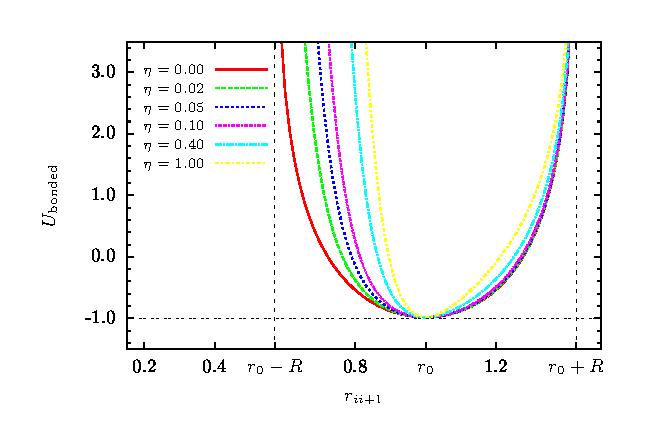
\includegraphics[width=0.85\textwidth]{chapter6Figs/bondedInter.eps}\hspace{2pc}%
\caption{\label{fig:modifiedBondedPotential} The modified bonded potential $U_{\mathrm{bonded}}(r_{ii+1})$, represented by the FENE and Lennard-Jones interactions. The strength of the LJ term is controlled by the parameter $\eta \in [0,1]$.}
\end{figure}

\newpage
In order to overcome the challenges associated with the simulation of polymers at very low energies, a parallel version of multicanonical sampling \cite{muca1a,muca2,Zierenberg2013} has been used in this study. In this method, $K$ independent multicanonical runs are performed in parallel. The initial estimates for the multicanonical weight functions are the same for all replicas. However, the random number generators are initialized with different seeds which allows each replica to perform a unique random walk in the energy space. Displacement updates are proposed within a cubic box of edge lengths $d=0.3r_0$ and accepted according to the probability
%
\begin{equation}
P(\mathbf{{X}} \rightarrow \mathbf{X}')= \mathrm{min}[1,W(E( \mathbf{X}'))/W(E( \mathbf{X}))],
\end{equation}
%
where $W(E( \mathbf{X}))$ represents the multicanonical weight of a given configuration $ \mathbf{X}$. After the $i$th iteration, since the weights are identical in each thread, the energy histograms obtained for each replica can simply be summed up:
%
\begin{equation}
    H^i(E)=\sum^K_{k=1}H^i_k(E). 
\end{equation}
%
The combined histogram is then used together with the current multicanonical weights to calculate the weights for the subsequent iteration by utilizing the error-weighted recursive
scheme~\cite{Bachmann2014,muca1a,muca2}. 

To analyze the transition behavior of the polymer chains for different values of the parameter $\eta$, we use the microcanonical inflection-point analysis~\cite{Bachmann2014,Schnabel2011} which has been introduced in Sec.~\ref{subsec: micro_analysis}. By applying the principle of minimal sensitivity~\cite{Stevenson} to the derivatives of the microcanonical entropy $S(E)$, the application of this method can be extended to higher order pseudophase transitions. The $(2n+1)$th-order transition ($n$ is a positive integer) is identified from the least sensitive inflection point of the $2n$th-derivative of entropy and the positive valley in the $(2n+1)$th-derivative curve. For a $2n$th-order transition, the least sensitive inflection point in the $(2n-1)$th-derivative of entropy together with the negative peak in the $2n$th-order derivative curve are utilized to locate the transition energy. 
%
%%%%%%%%%%%%%%%%%%%%%%%%%%%%%%%%%%%%%%%%%%%%%%%  
%%%%%%%%%%%%%%%%%%%%  RESULTS		         %%%%%%%%%%%%%%%%%
%%%%%%%%%%%%%%%%%%%%%%%%%%%%%%%%%%%%%%%%%%%%%%%
\section{Results}
%
In the following, we investigate the effects of bond asymmetry and short range repulsion on the thermodynamic and structural properties of elastic polymers of length $N=15,55$.  We begin with a discussion of the results of canonical analysis, which provides a general picture of the transition behavior. The order and the exact location of each pseudophase transition is obtained by the means of the microcanonical inflection point analysis, and the results are used to construct pseudophase diagrams. 

%%%%%%%%%%%% CANONICAL RESULTS %%%%%%%%%%%%%%

\subsection{Canonical results}
In canonical analysis, extremal thermal fluctuations of a thermodynamic observable $O$, defined as
%
\begin{equation}
    \frac{d}{d T}\langle O\rangle = \frac{1}{k_{\rm B}T^2} \left[ \langle O E 
    \rangle-\langle O\rangle\langle E\rangle \right],
    \label{eq:fluctuation}
\end{equation}
%
are used to locate regions of increased thermal activity associated with pseudophase transitions. The most commonly considered observable is the energy $E$, and its thermal fluctuation, the heat capacity $C_{\mathrm{V}}$, is useful for identifying transitions in complex systems. 

The heat-capacity curves for a 15mer and a 55mer are shown in Fig.~\ref{fig:canonicalAnalysis}~(a,b) as functions of the canonical temperature $T$. In the case of the 15mer, prominent wide peaks at $T \approx 0.34$ indicate the freezing transition at which expanded globular structures change to more compact crystalline or amorphous structures. For $\eta < 0.1$, additional peaks below the freezing transition suggest the existence of a possible solid-solid transition when the short-range repulsion of the bonded interactions is sufficiently weak. With increasing $\eta$, the strength of the transition increases as it shifts towards lower temperatures, and eventually disappears at $\eta \approx 0.1$. 

The freezing transition of a 55mer at $\eta = 1$ is a prominent example of a first-order pseudophase transition. In Fig.~\ref{fig:canonicalAnalysis}~(b), this corresponds to the pronounced peak at $T \approx 0.325$. However, the peaks become broader and less pronounced as $\eta$ decreases. Eventually, they are no longer associated with a single transition, but rather envelope multiple transition signals. This ambiguity in distinguishing and classifying the transitions at small $\eta$ values is caused by finite-size effects which cannot be resolved by means of canonical statistical analysis. It is necessary to employ other systematic and robust methods which can clearly distinguish the sensitive transition signals in finite-size systems.  
%
\begin{figure}
\center
    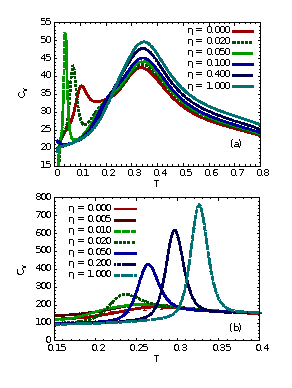
\includegraphics[width=0.6\textwidth]{chapter6Figs/canonicalAnalysisRough.eps}%
    \caption{\label{fig:canonicalAnalysis}
	Heat capacity $C_{\mathrm{v}}$ for elastic polymer chains of length $N=15$ (a), and $N=55$ (b), with modified bonded potential and different values of the control parameter $\eta$.}
\end{figure}
%

%%%%%%%%%%%% MICROCANONICAL RESULTS %%%%%%%%%%%%%%
\subsection{Microcanonical results and structural phase diagrams}

Here we examine in detail the transition behavior of the polymer chains for representative values of the $\eta$ parameter in the interval $\eta\in[0,1]$. The combined microcanonical results are shown in Fig.~\ref{fig:microcanonicalAnalysis} for a $15$mer (a,c,e) and a $55$mer (b,d,f). Closer inspection of the derivatives of the microcanonical inverse temperature $\beta(E)$ of the 15mer, reveals two distinct transition signals inside the energy interval $E\in[-44,-38]$. At $E\approx -44$, the least sensitive point of $\delta(E)$ indicates a fourth-order transition. The second transition, located at $E\approx -38$, is of a second-order for $\eta > 0.2$ and third-order for $\eta < 0.2$. In the canonical picture, both signals would be enclosed within the broad peaks of the heat capacity $C_{\mathrm{V}}$ (Fig.~\ref{fig:canonicalAnalysis}), concealing the fact that the freezing transition is a two step process. The two-step freezing transition is also observed in the case of the $55$mer, for $\eta=0.05, 0.2$, and $1$. The prominent back-bending features in the microcanonical inverse temperature $\beta(E)$ accompanied by the positive-valued peaks in $\gamma$ are clear indicators of a first-order transition. The peaks in $\gamma(E)$ are accompanied by inflection points located at $E \approx -247, -242, -235,$ and $-229$ for $\eta= 0.05, 0.20,$ and $1.00$ respectively. Together with the corresponding positive valleys in $\delta(E)$, these inflection points indicate additional third-order transitions. For $\eta < 0.03$, the properties of the freezing transition change as additional pseudophases emerge and the transition is extended over a wide energy region. 

For the 15mer at $\eta \leq 0.1$, clear signals corresponding to a solid-solid transition are detected. For $\eta=0.00$, third-order solid-solid transition is indicated by the inflection point in $\gamma(E)$ at $E=-48.92$ and the corresponding positive valley in $\delta(E)=d \gamma(E)/d E$. For $\eta=0.02$ and $0.05$, the negative-valued peaks in $\gamma(E)$ indicate a second-order transition at $E=-49.7$ and $-50.4$ respectively. Whereas for $\eta \geq 0.1$, no solid-solid transition signals are detected.

%
\begin{figure}
\center
    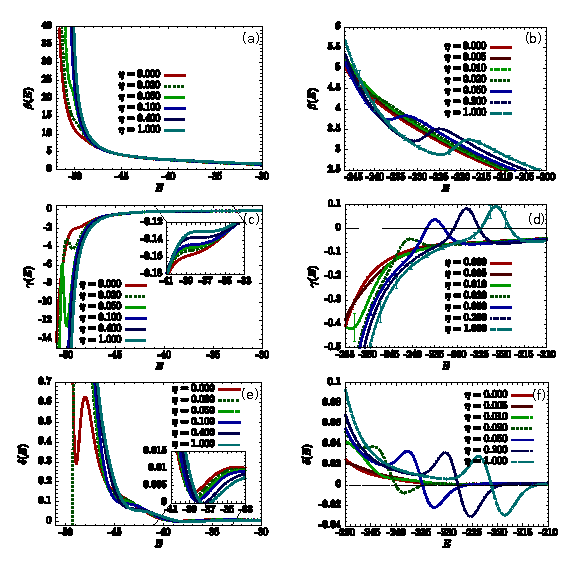
\includegraphics[width=1.0\textwidth]{chapter6Figs/microcanonicalAnalysis.eps}%
    \caption{\label{fig:microcanonicalAnalysis}
	The combined microcanonical results for the $15$mer (a,c,e) and the $55$mer (b,d,f), for representative values of the parameter $\eta$ in the range $\eta\in[0,1]$.}
\end{figure}
%

\newpage
Using the signals obtained from microcanonical inflection-point analysis, we have constructed structural phase diagrams shown in Figs.~\ref{fig:phaseDiagram15} and~\ref{fig:phaseDiagram55} for the $15$mer and the $55$mer respectively. At high energies and temperatures, polymer chains are found in the the gas-like pseudophase (G) in which expanded random-coil structures dominate. With decreasing temperature and energy, the expanded chains collapse into the liquid pseudophase (L) which consists mainly of globular structures. The corresponding pseudophase transition is the well-known $\Theta$-transition (collapse transition). For both system sizes, the $\Theta$ transition is classified as second-order and is represented by blue lines in the phase diagrams.

%
\begin{figure}
\center
    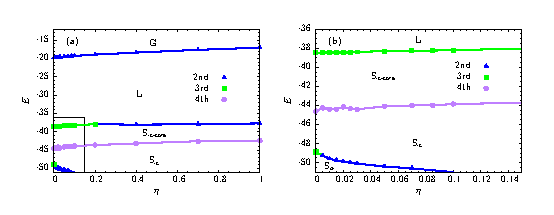
\includegraphics[width=\textwidth]{chapter6Figs/phaseDiag15.eps}%
    \caption{\label{fig:phaseDiagram15} 
    (a) Microcanonical pseudophase diagram for the $15$mer,  parametrized by energy and the control parameter $\eta$. The labels G, L, and S stand for ``gas'', ``liquid'', and ``solid'' pseudophases, respectively. The $S_{\mathrm{ic-core}}$ pseudophase consists of icosahedral structures with an unstable liquid-like surface layer. The $S_{\rm ic}$ and $S_{\rm bi}$ pseudophases are dominated by stable icosahedral and bihexagonal structures. (b) Expanded section detailing the low energy region for $\eta < 0.15$.}
\end{figure}
%
\begin{figure}
\center
    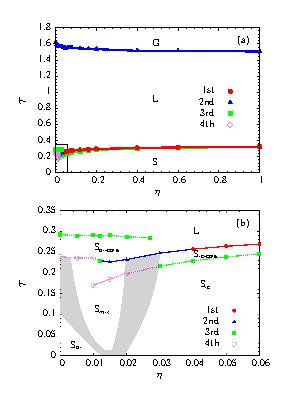
\includegraphics[width=0.70\textwidth]{chapter6Figs/phaseDiag55.eps}%
 	\caption{\label{fig:phaseDiagram55} (a) Microcanonical pseudophase diagram for the $55$mer,  parametrized by temperature and the control parameter $\eta$. The labels G, L, and S stand for ``gas'', ``liquid'', and ``solid'' pseudophases, respectively. (b) Expanded section detailing the low temperature region for $\eta < 0.06$. The $S_{\mathrm{ic-core}}$ and $S_{\mathrm{bi-core}}$ pseudophases consist of structures with icosahedral and bihexagonal cores, respectively, and unstable liquid-like surface layers. The $S_{\rm ic}$ and $S_{\rm bi}$ pseudophases are dominated by stable icosahedral and bihexagonal structures with complete shells. In $S_{\mathrm{mix}}$ both icosahedral and bihexagonal core structures are represented. The ``solid'' subphases are separated by gray empirical transition bands. Dashed lines represent lines of transitions higher than second order.}
\end{figure}

With further decrease in energy, the 15mer passes the second/third-order transition associated with the nucleation process, and enters the $S_{\rm ic}$ pseudophase in which icosahedral structures with unstable surface layer are dominant. At even lower energies $(E \approx -44)$, the thermal fluctuations of the polymer are suppressed and a stable surface layer is formed. The transition associated with the surface formation process is of fourth order. Visual inspection of low-energy structures reveals that icosahedral geometries are dominant. However, for $\eta \leq 0.1$, the additional solid-solid transition suggests the existence of low-energy conformations with unexpected bihexagonal geometries (Fig.~\ref{fig:coreStructures}).

The transition behavior of the $55$mer is qualitatively similar to the $15$mer for the majority of values of the $\eta$ parameter. However, for $\eta < 0.1$ the two systems behave differently. The low-temperature and small-$\eta$ region of the structural phase diagram in Fig.~\ref{fig:phaseDiagram55}, contains additional transition lines which were not detected for the $15$mer. The emergence of the third-order transition line at $T \approx 0.29$ for $\eta < 0.03$, marks the end of a clear distinction between the liquid and solid pseudophases. The nucleation process becomes extended over a wide temperature range and can't be associated with a single transition line. Instead, the polymer transitions between several conformational phases before it forms a stable ground state structure. We will identify and characterize the dominant conformational phases using a set of suitable structural order parameters\footnote{See also section ~\ref{sec:orderParameters}}.
 

%%%%%%%%%%%%%% STRUCTURAL ANALYSIS %%%%%%%%%%%%%%%%%%
\subsection{Structural analysis}
%
The tools of microcanonical inflection-point analysis provide us with a systematic way of identifying and classifying all structural transitions in physical systems. Equally important is the identification of dominant configurations and their abundance in a relevant energy range. This can be accomplished either by visual inspection of sample structures, or more systematically, by introducing a suitable set of structural order parameters. Based on the microcanonical results, summarized in the structural phase diagrams in Figs.~\ref{fig:phaseDiagram15} and.~\ref{fig:phaseDiagram55}, we expect that for sufficiently small values of the parameter $\eta$, two distinct solid pseudophases should be detected. We aim to identify and characterize the dominant structures for each pseudophase and obtain a physical interpretation for the emergence of new conformational geometries when the short-range repulsion between bonded monomers becomes sufficiently weak. In Chap.~\ref{chap:HomopolymerModel}, we have introduced a set of structural order parameters $Q_{l}$ which are particularly suitable for the purpose of identification of low-energy solid-like structures with well-defined symmetries.
%

%
Preliminary investigation of low-energy structures, obtained from simulations of polymer chains of length $N =15,55$ with sufficiently weak bonded Lennard-Jones interactions $(\eta < 0.03)$, reveals the existence of two distinct solid pseudophases. In addition to structures with icosahedral cores, we have identified bihexagonal cores with six-fold dihedral symmetry. Examples of both core geometries are shown in Fig.~\ref{fig:coreStructures}.
%
\begin{figure}
\center
	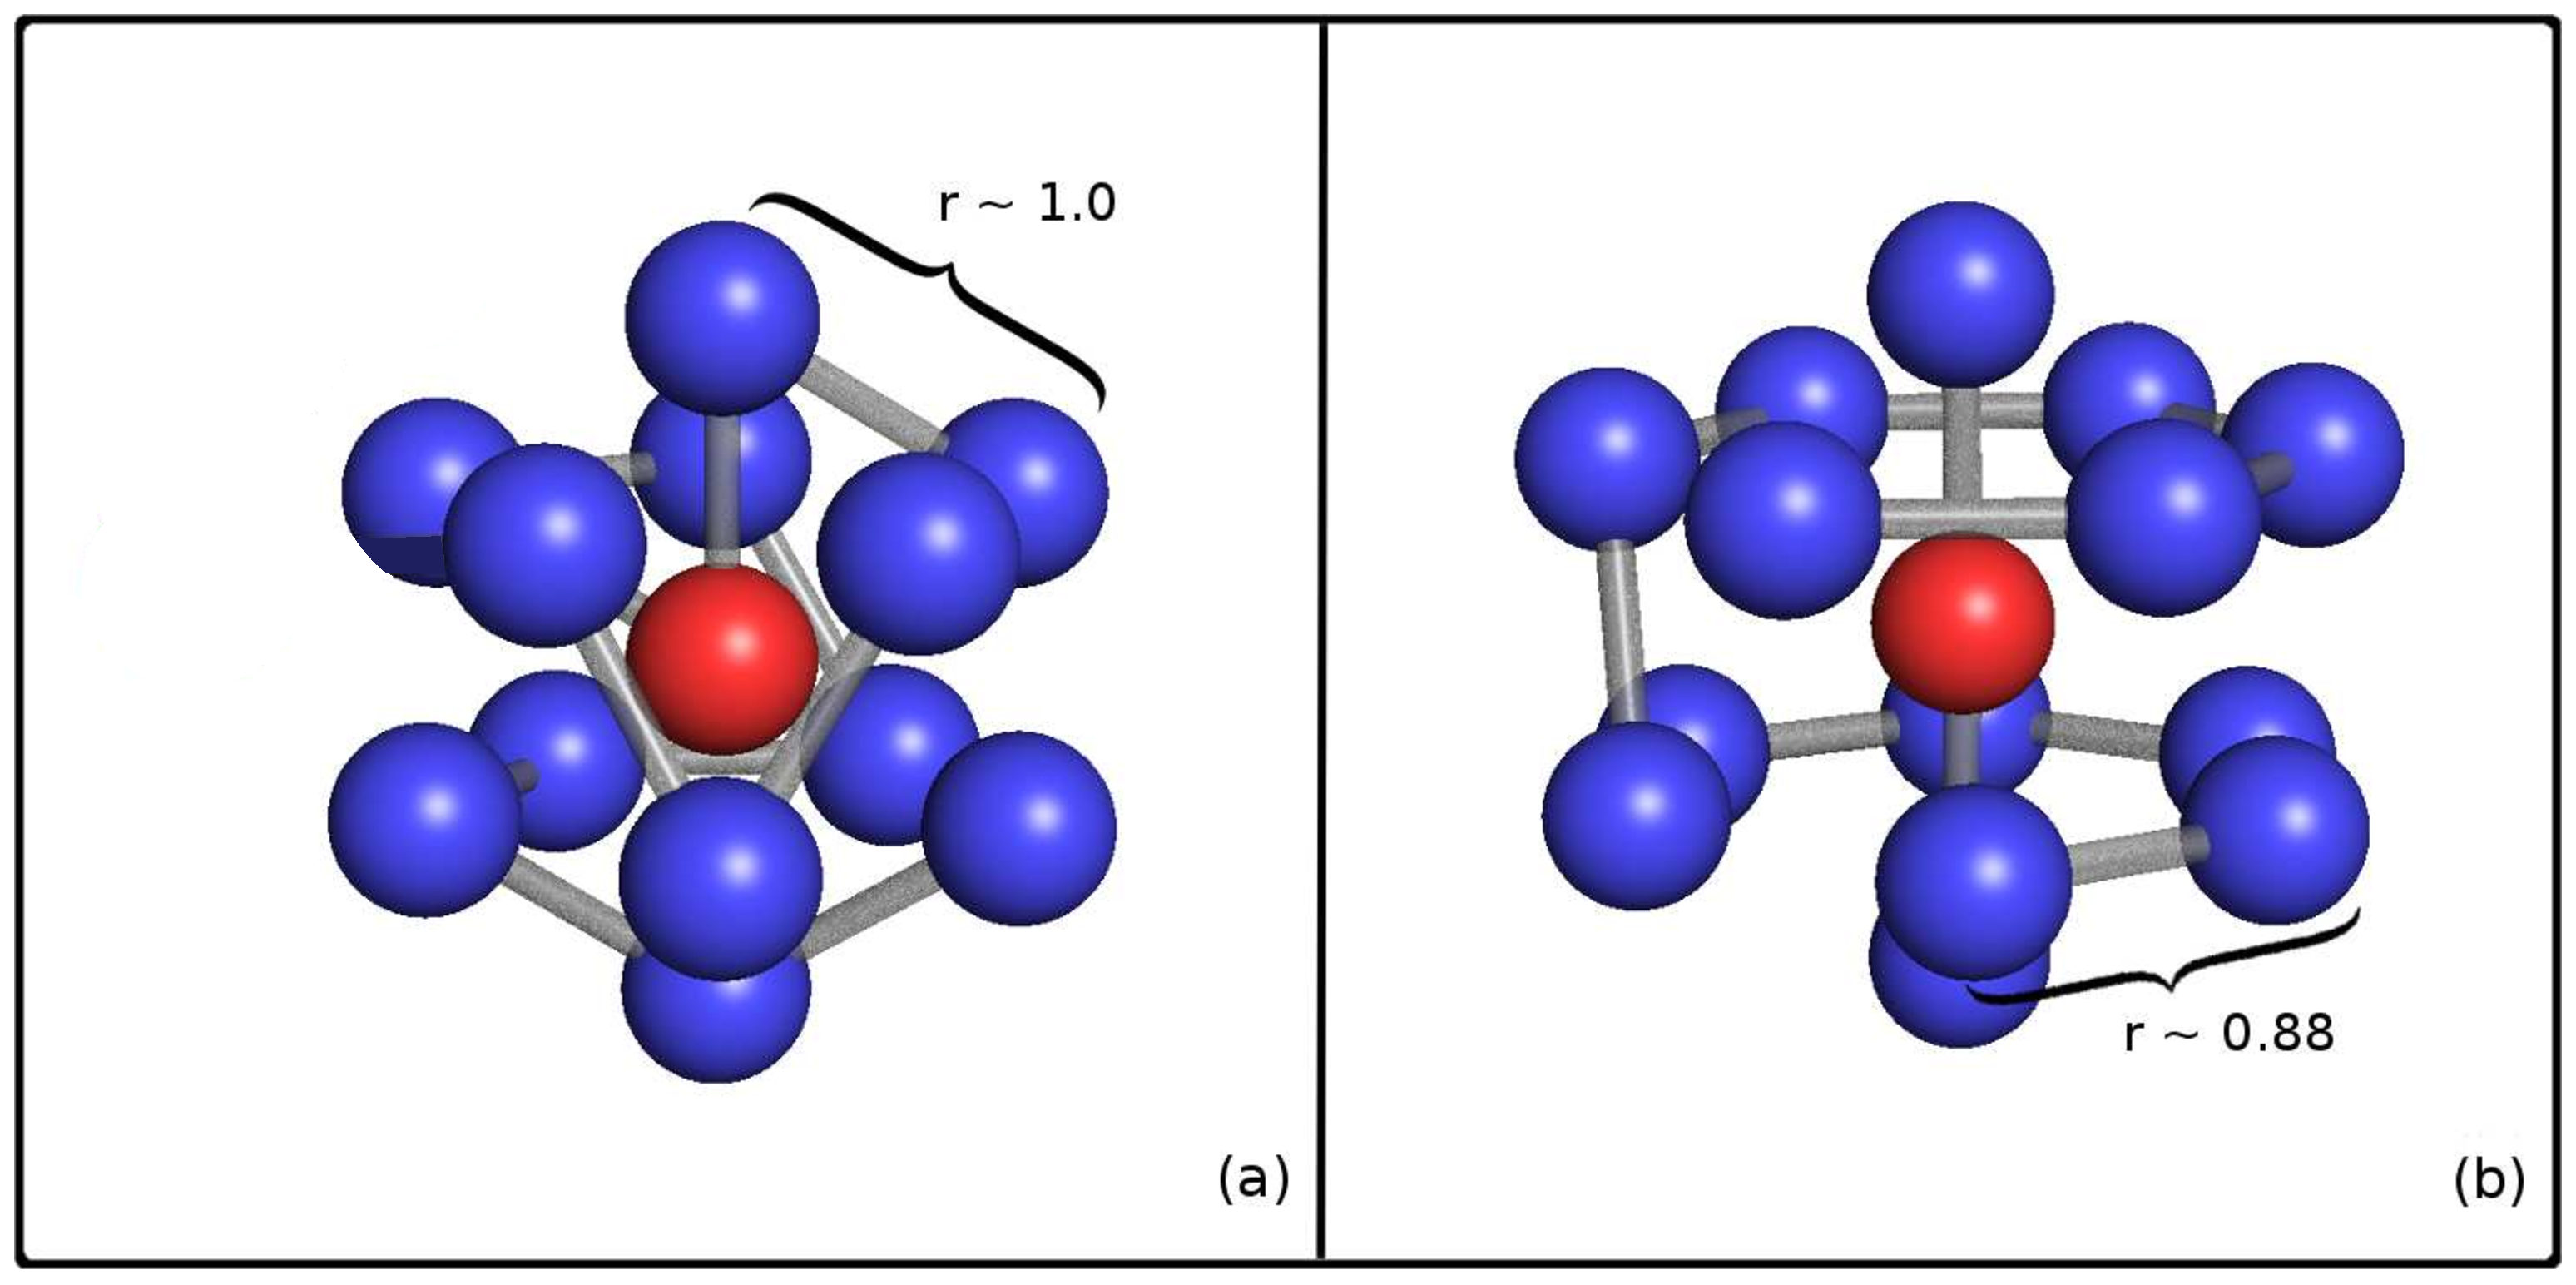
\includegraphics[width=0.9\textwidth]{chapter6Figs/configurationsMod.eps}			\caption{\label{fig:coreStructures} Two distinct core geometries found in the low-energy states of elastic polymer chains of lengths $N = 15,55$. (a) The 13-monomer icosahedral core is commonly observed in the ground state structures of short polymer chains. (b) The unusual bihexagonal core is found in polymer chains of length $N =15,55$ with sufficiently weak bonded Lennard-Jones interactions.}
\end{figure}
%
Using $\sim 10^{6}$ polymer structures per value of $\eta$, we have computed $Q_{l}$ up to $l = 8$ and found that $Q_{6}$ is most effective in resolving the six-fold dihedral symmetry of the bihexagon and the icosahedral symmetry. For a bihexagonal core $Q_{6} \approx 0.41$, and the icosahedral core corresponds to $Q_{6} \approx 0.65$. The results are presented in the form of intensity plots in Figs.~\ref{fig:intensityPlots15} and~\ref{fig:intensityPlots55}, for the 15mer and the 55mer, respectively. The probability $p$ of detecting a conformation with a specific value of the order parameter $Q_{6}$ is represented by shading; red indicates the maximum probability $p=1$ and black corresponds to $p=0$.
%

%
For $\eta > 0.1$, the 15mer has a single solid pseudophase which is predominantly populated by structures with stable icosahedral cores. In Fig.~\ref{fig:intensityPlots15} this corresponds to the narrow funnel centered at $Q_{6} \approx 0.65$, below the fourth-order transition line (purple) at $E \approx -43$. An additional solid pseudophase, consisting mostly of bihexagonal structures, emerges for $\eta \leq 0.1$, as indicated by the appearance of a second funnel centered at $Q_{6} \approx 0.41$. The region of coexistence between the two solid pseudophases marks the solid-solid transition (dashed lines) and is in a good agreement with the microcanonical estimates. 
%

%
Similarly, in the case of the 55mer, we detect a single solid pseudophase for $\eta \geq 0.02$, populated with structures containing icosahedral cores. For $\eta \geq 0.04$, the microcanonical signal associated with the freezing transition becomes first-order (Fig.~\ref{fig:phaseDiagram55}). This nicely corresponds with the abrupt onset of the icosahedral funnel in Fig.~\ref{fig:intensityPlots55} (d). However, unlike the 15mer, the 55mer does not have an identifiable icosahedral pseudophase for $\eta \leq 0.005$. In Fig.~\ref{fig:intensityPlots55} (a), the wide dominant funnel, centered at $Q_{6}\approx 0.41$, contains exclusively structures with bihexagonal cores. The fourth-order transition signal, represented by the dashed violet line in the structural phase diagram in Fig.~\ref{fig:phaseDiagram55}, corresponds to the increase in the population of structures with bihexagonal cores at $T \approx 0.24$. The population of structures with icosahedral cores grows quickly with the increasing strength of the bonded LJ potential. For $\eta = 0.01$ (Fig.~\ref{fig:intensityPlots55} (b)), the ground state structures are found exclusively inside of the bihexagonal funnel. However, the onset of prominent icosahedral funnel at $T = 0.17$ creates an additional fourth-order transition signal. 
%   

Further increase leads to a sharp decline in the population of the bihexagonal funnel. 

for $\eta \geq 0.02$ [Fig.~\ref{fig:intensity_plots}(c), (d)] where the energetic penalty for non-optimal bond lengths becomes too large to accommodate structures with bihexagonal cores. Indeed, their formation requires significant variance in bond lengths, whereas icosahedral cores can be formed with near-optimal values. For $\eta\approx 0$, the pure FENE potential permits large bond fluctuations. However, with the introduction of the bonded LJ potential these fluctuations cause an energetic penalty. This explains why the bihexagonal funnel exists only if the bonded LJ potential is sufficiently weak. 

%
The shape of the bonded potential has undoubtedly a strong effect on
the geometry of the ground state. Having identified the two dominant
structure types, we may ask why the additional LJ term in the bonded
potential eventually precludes the existence of the bihexagonal phase. The
answer is readily obtained by comparing the average bond lengths for the
icosahedral and bihexagonal structures. The bihexagon accommodates all
monomers into a single shell allowing for a larger number of non-bonded
interactions and consequently lower energy. However, the two six-monomer
rings of the bihexagon contain significantly compressed bonds
$(r_{\mathrm{bond}} \approx 0.88 r_{0})$, which become energetically
infeasible as $\eta$ increases. In contrast, we find near-optimal bond
lengths in the icosahedron $(r_{\mathrm{bond}} \approx  r_{0})$, hence the
``narrowing'' of the bonded potential imposes no additional energetic
penalty.




%
\begin{figure}
\center
	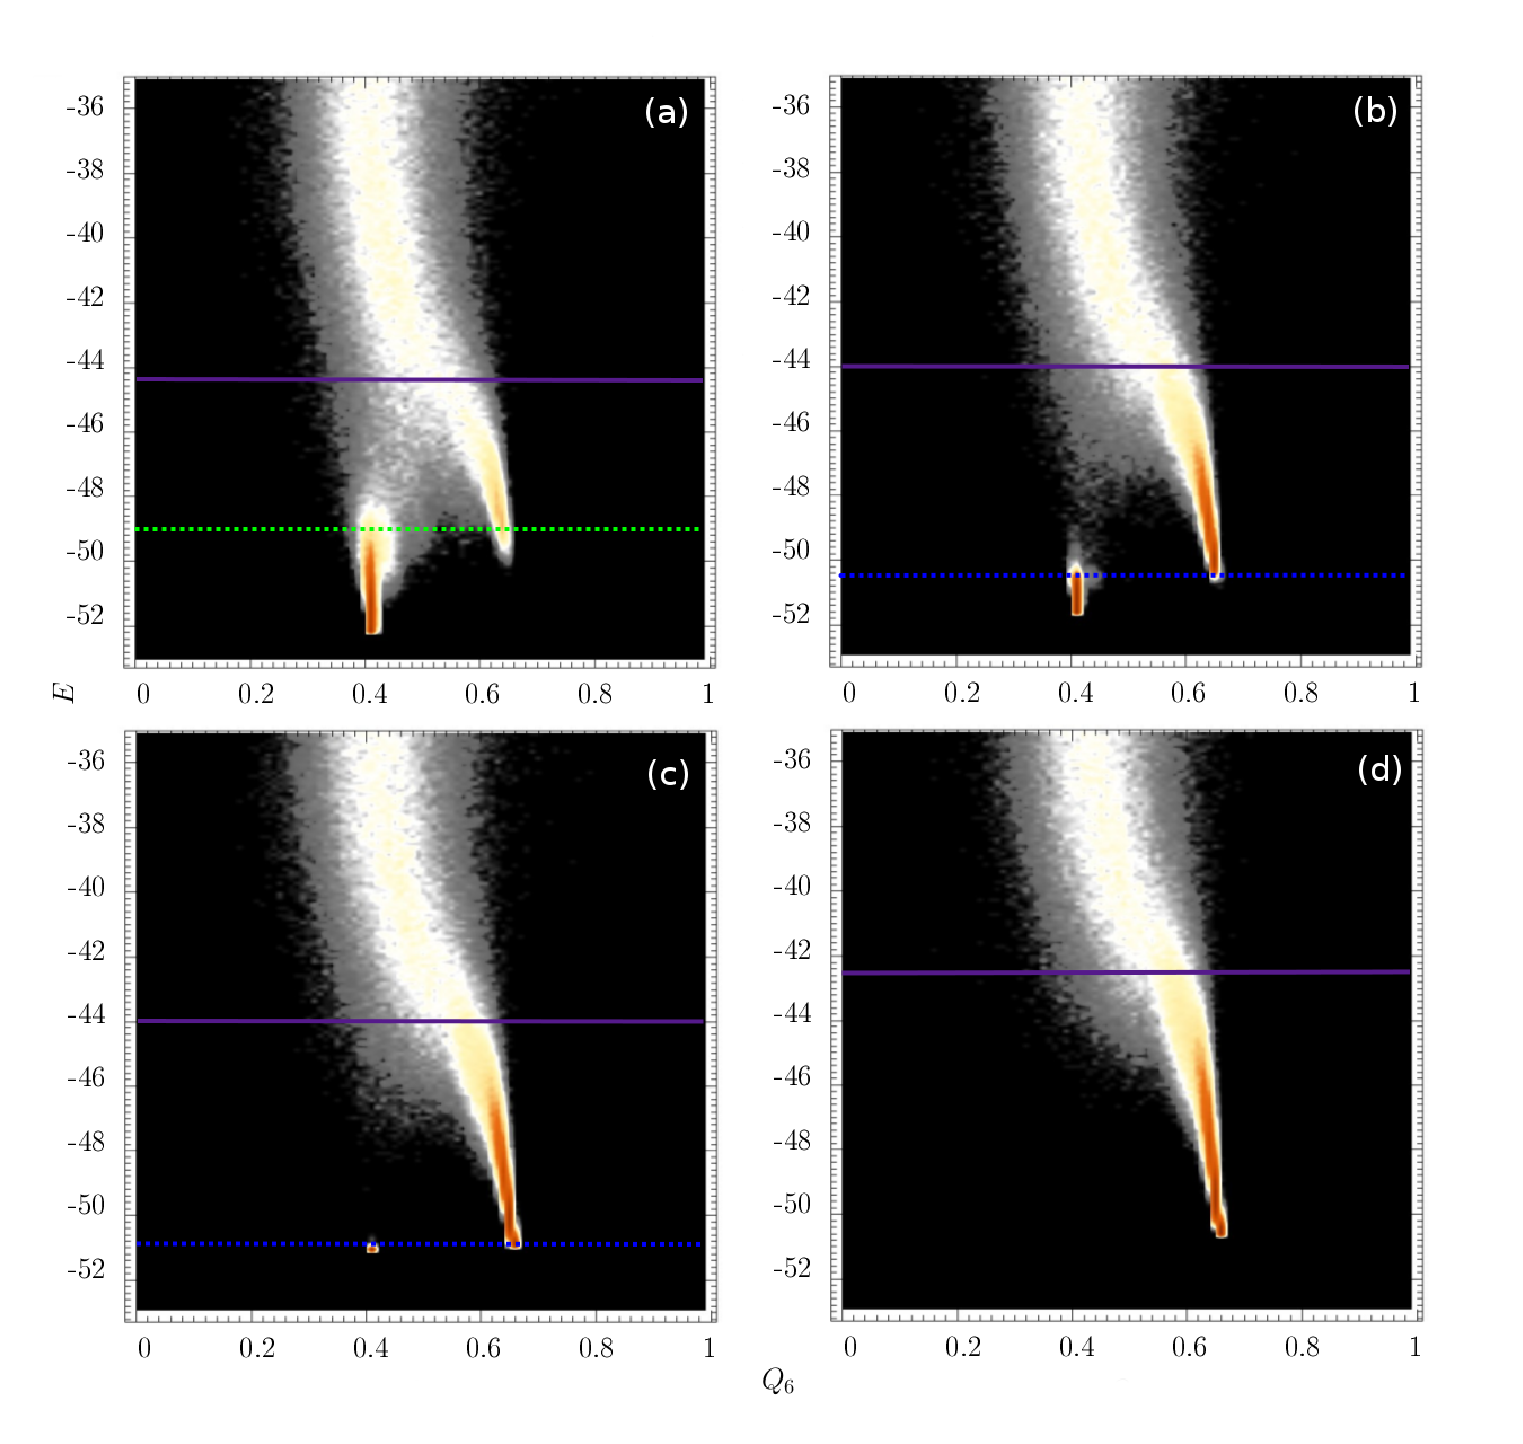
\includegraphics[width=\textwidth]{chapter6Figs/structuralAnalysis15.eps}
\caption{\label{fig:intensityPlots15}(a,b,c,d) Intensity plots of the
$Q_{6}$ order parameter for a 15mer with $\eta = 0.00, 0.05, 0.10, 1.0$.
The shading indicates the probability of detecting a configuration with a
given value of the order parameter, red being the maximum probability and
black being the lowest. The freezing and the solid-solid transitions are
indicated by solid and dashed horizontal lines respectively. For $\eta \leq
0.1$, the polymer has two distinct solid phases.  In addition to the
icosahedral phase ($Q_{6} \approx 0.65$) the polymer is found in the
bihexagonal phase at low energies ($Q_{6} \approx 0.41$).}
\end{figure}
%
%
\begin{figure}
\center
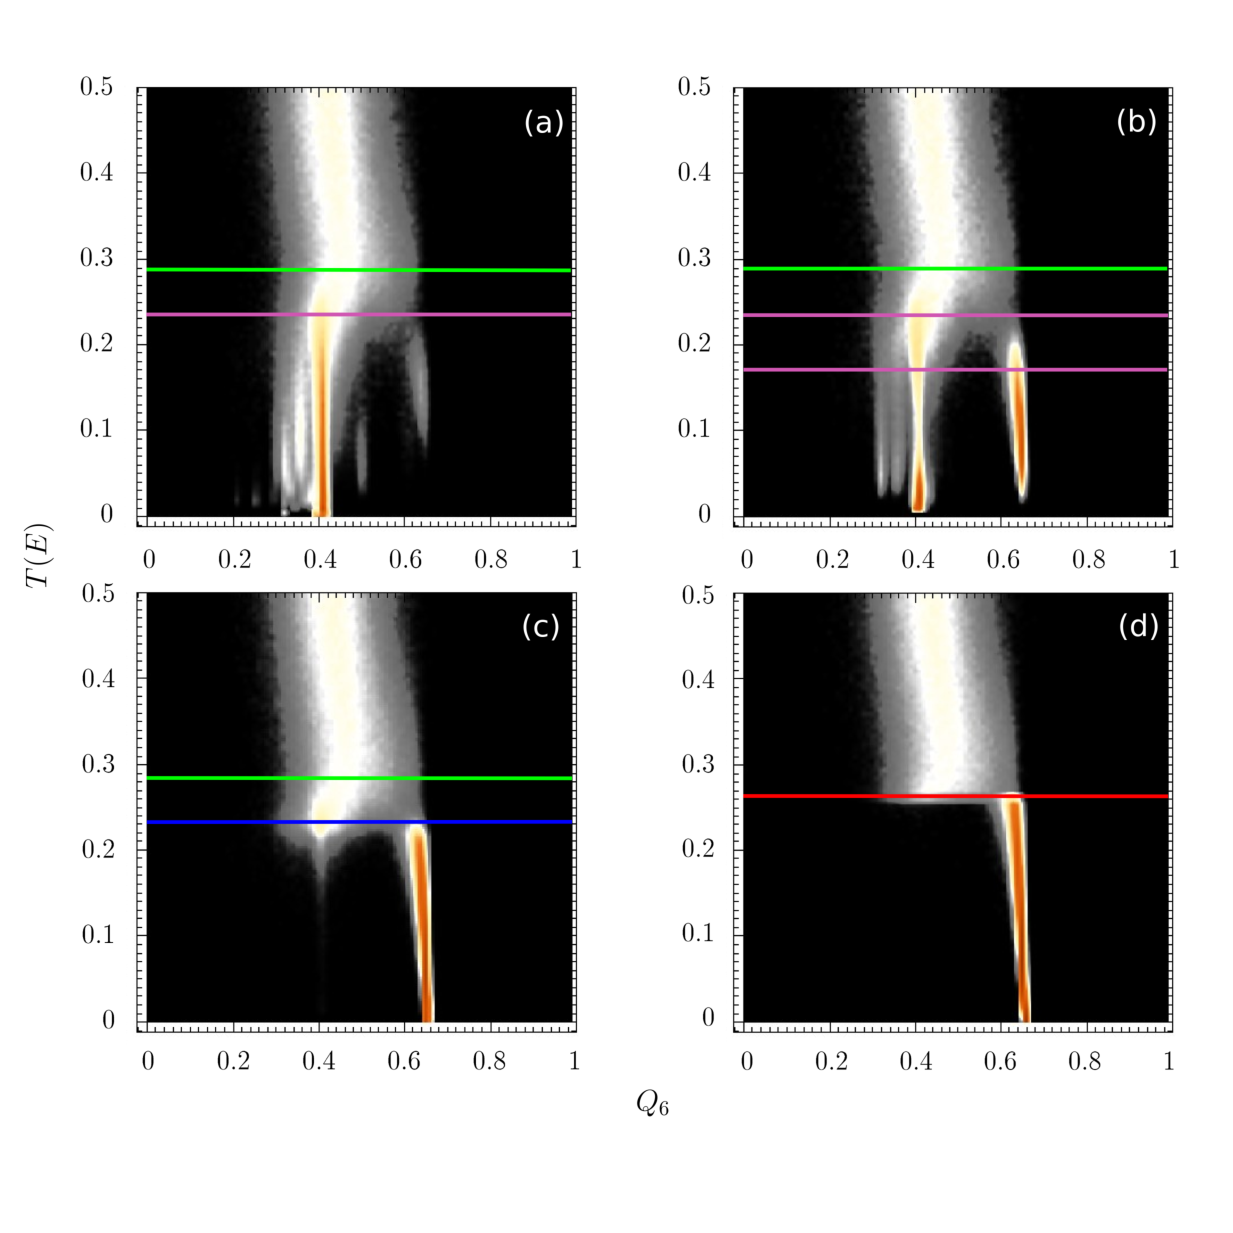
\includegraphics[width=\textwidth]{chapter6Figs/structuralAnalysis55.eps}
	\caption{\label{fig:intensityPlots55}
     sdfdf}
\end{figure}



%%%%%%%%%%%%%%%%%%%%%%%%%%%%%%%%%%%%%%%%%%%%%%%%%%%%%%%%  			          SUMMARY		               %%%%%%%%%%%%%%%%
%%%%%%%%%%%%%%%%%%%%%%%%%%%%%%%%%%%%%%%%%%%%%%
\section{Summary}
%
We have investigated the thermodynamic and structural behavior of a coarse-grained model of an elastic homopolymer chain of length $N=15,55$, upon changing the model parameter $\eta$ which controls the strength of the bonded LJ potential. For small values of this parameter, a freezing transition into an icosahedral phase precedes a solid-solid transition into low-energy states with bihexagonal geometry. The non-optimal bond lengths found in bihexagonal
conformations cause a large energy penalty due to the ``narrowing'' of the
bonded potential if $\eta$ is increased. Hence only a single
solid phase remains for $\eta > 0.1$, which is icosahedral. The striking
consequences of a relatively small modification to the standard model of
elastic, flexible homopolymers illustrate the importance of a careful
choice of model parameters.




\chapter{Aggregation of Flexible Elastic Homopolymers}
\label{chap:Aggregation}
\section{Introduction}
%
Deeper understanding of aggregation processes in the context
of microscopic molecular systems is relevant for a number of 
technological and biomedical applications. For example,
protein aggregation is believed to play a critical role during
the onset of many prominent pathological conditions, 
such as cystic fibrosis, Alzheimer's and Parkinson's
diseases~\cite{Selkoe,Chiti}. The staggering complexity of even the 
simplest molecular systems precludes the possibility of obtaining 
the relevant thermodynamic quantities through direct analytical 
calculations~\cite{Bachmann2014}. Over the past two decades, 
the enormous increase in the availability of computational resources, 
together with significant progress in algorithmic developments, 
resulted in a vast number of computational studies on the thermodynamic 
and structural properties of complex microscopic systems. 
Among the most efficient simulation methods are the
generalized-ensemble Monte Carlo algorithms, such as
simulated tempering~\cite{marinari,lyubartsev},
replica-exchange parallel tempering~\cite{sw1,geyer1,huku1,huku2}, 
multiple Gaussian modified ensemble (MGME)~\cite{Neuhaus2006}, 
together with
multicanonical~\cite{muca1a,muca1b,muca2,muca3,muca4,Bachmann2013}
and Wang-Landau sampling~\cite{wl1,wl2,wl3}. 
These have been applied successfully in numerous studies of 
structural phases and transition
properties~\cite{Schnabel2009,bf1,bf2,grass2,vbj1,strauch1,svbj1,%
taylorRange1, taylorRange2,seaton3,semisslb1,Koci2015}, surface
adsorption~\cite{bj4,prellberg1,paul1,mbj1,liang1,allen1,vb1,ywli1,%
mjb4,vgb1}, and
aggregation~\cite{jbj1,Junghans2008,Junghans2009,Junghans2011,%
Zieren2014,Zieren2015} of generic off-lattice homopolymers and
heteropolymers. The folding properties of coarse-grained protein models
have also been examined
extensively~\cite{dill1,still1,still2,som1,hsu1,bj1,ssbj1}.
 
Importantly, despite the many advances in simulational
methodologies, systematic studies of detailed atomistic
models are well beyond current capabilities. 
However, it is a significant physical reality that many 
essential thermodynamic properties of complex systems are 
retained on larger than atomistic scales and can be well represented 
by coarse-grained models. In fact, coarse-graining is not just a concept
to simplify modeling. It reflects inherent collective and cooperative
behavior of constituents of systems on mesoscopic and macroscopic scales. 
This is intuitive since it is known that certain characteristic
properties, such as the propensity towards aggregation, are often shared
among diverse systems and hence cannot depend sensitively on microscopic
details.
 
In mesoscopic systems, structure formation and phase-separation
processes are fundamentally influenced by finite-size effects.
Systematic statistical analysis approaches beyond the standard
canonical methodology are needed to unravel the intricate details
of the interplay between energy and entropy in finite systems.
Due to the averaging process involved in the calculation of 
canonical quantities such as the ensemble energy or the heat capacity,
specific features of structural transitions and phase properties 
are often lost~\cite{Bachmann2014}. This is remedied in more general 
approaches such as the Fisher partition 
zeros~\cite{fisher1,taylor1,rslb1,taylor2}, 
or the microcanonical inflection-point 
analysis~\cite{Schnabel2011,KaiQi2016}.

This paper is organized as follows: In Sect.~\ref{sec:modmeth},
we introduce a coarse-grained model for interacting flexible
elastic homopolymers, describe the employed computational methods, 
and briefly outline the methodologies of the microcanonical 
inflection-point analysis. In Sect.~\ref{sec:res}, we present
the simulational results for polymer systems of up to $M =20$
chains. Based on the outcome of inflection-point analysis,
we argue that the aggregation transition is a first-order process 
consisting of a sequence of subtransitions between intermediate 
structural phases. Next, we discuss why certain subphases
are entropically more suppressed than others, and conclude
with a brief excursion into the scaling properties of the aggregation
transition temperature and the latent heat. Summary is provided
in Sect.~\ref{sec:sum}.
%
%%%%%%%%%%%%%%%%%%%%%%%%%%%%%%%%%
%%%%%%%%%%% METHODS %%%%%%%%%%%%%%%%
%%%%%%%%%%%%%%%%%%%%%%%%%%%%%%%%%
\section{Model and Methods}
\label{sec:modmeth}
%
In the following, we introduce a generic coarse-grained model
for a system of interacting, flexible homopolymers. Coarse-grained models,
with a suitably chosen set of
parameters, drastically reduce computational complexity while
preserving the essential structural and thermodynamic properties
that are typically found in more complex
models~\cite{Schmid2011}.
%
\subsection{Standard model of interacting elastic chains}
%
In this study, we investigate the aggregation of
$M$ interacting flexible homopolymers, each composed of
$N = 5$ monomers. During the simulations, the system is constrained
inside of a steric sphere at a constant density of $10^{-3}$
monomers per unit volume. At this density the radius of the
constraining sphere is larger than the length of the fully
extended polymer chains under investigation. The total energy of
the system can be separated into intra-chain and inter-chain
pairwise interactions
%%%%%%     Total Energy      %%%%%%
\begin{equation}
E_{\mathrm{total}} = E_{\mathrm{intra}} + E_{\mathrm{inter}}.
\end{equation}
%
The intra-chain contribution 
%%%%%% Intra-Chain Energy %%%%%%%
\begin{equation}
E_{\mathrm{intra}} = \sum^{M}_{k = 1}\sum^{N-1}_{i = 1}
U_{\mathrm{FENE}}(r\,^{(k)}_{ii+1}) +
\sum^{M}_{k=1}\sum^{N}_{i<j}
U_{\mathrm{LJ}}^{\mathrm{trunc}}(r\,^{(k)}_{ij})
\end{equation}
%
consists of both bonded and non-bonded interactions, where
$r\,^{(k)}_{ij}$ is the distance between the pair of monomers
($i$,$j$) of the $k$-th chain. The first term contains the anharmonic
finitely extensible nonlinear elastic (FENE)
potential~\cite{Bird1987, Kremer1990, Milchev2001}
%%%%%% FENE Potential %%%%%%
\begin{equation}
U_{\mathrm{FENE}}(r_{ii+1})=-\frac{K}{2}R^2 
\mathrm{ln}\left[1-\left(\frac{r_{ii+1}-r_0}{R}\right)^2\right],	
\label{FENE}
\end{equation}
%
with parameter values $K=40$ and $R=0.3$ as used in~\cite{Gross2013}.
The second term represents 
the truncated and shifted Lennard-Jones (LJ) potential
%%%%%% LJ Potential %%%%%%
\begin{equation}
U_{\mathrm{LJ}}^{\mathrm{trunc}}(r_{ij}) = \left\{
\begin{array}{lr}
U_{\mathrm{LJ}}(r_{ij}) - U_{\mathrm{LJ}}(r_{c}), & \quad
\mathrm{if} \,\, r_{ij} \leq r_{c},\\
0, &  \quad \mathrm{if} \,\,r_{ij} > r_{c},
\end{array}
\right.
\end{equation}
%
where
%%%%%% LJ Potential %%%%%%
\begin{equation}
U_{\mathrm{LJ}}(r_{ij})= 4\epsilon \left[ \left(
\frac{\sigma}{r_{ij}} \right)^{12} - \left(
\frac{\sigma}{r_{ij}} \right)^{6} \right].
\end{equation}
%
We set the energy scale $\epsilon$ to unity and the length scale
to $\sigma=r_0/2^{1/6}$, where $r_0 = 0.7$ is the location of
the LJ potential minimum. The cutoff radius is set to
$r_c=2.5\,\sigma$.
The inter-chain contribution
%%%%%% Inter-Chain Energy %%%%%% 
\begin{equation}
E_{\mathrm{inter}} = \sum^{M}_{k < l}
\sum^{N}_{i,j}U_{\mathrm{LJ}}^{\mathrm{trunc}}(|\textbf{r}^{(k)}_{i}
- \textbf{r}^{(l)}_{j}|),
\end{equation}
%
consists solely of non-bonded LJ interactions. For the purpose
of this study, all LJ interactions (intra- and inter-chain) have
their parameters set to identical values.
%
\subsection{Simulation methods}
%
Relatively small polymer systems, consisting of $N < 100$
monomers, can be conveniently simulated using parallel tempering, which is
a generalized-ensemble
replica-exchange Monte Carlo method~\cite{sw1,geyer1,huku1,huku2} that can
be easily implemented on parallel
computer architectures. In larger systems, 
the density of states typically spans several
thousand orders of magnitude, in which case the application of more
sophisticated methods such as multicanonical
sampling~\cite{muca1a,muca1b,muca2,muca3,muca4,Bachmann2013} or 
Wang-Landau~\cite{wl1,wl2,wl3} is more efficient. In this study we restrict
our attention to systems consisting of up to $20$ individual chains with $5$
monomers each.
The number of monomers per chain has been intentionally kept very low 
in order to enhance translational entropic effects which become more 
obscured by the impact of inherent conformational
entropies as chain length is increased.

In a typical simulation, $R \approx 80$ replicas of the system were
simulated in parallel at different temperatures in the range 
$T \in \left[0.1,2.0\right]$.
Single-monomer random displacement moves, restricted to a box of size $l$,
were used to perform conformational updates for individual replicas.
The proposed update was then accepted with the Metropolis probability
%%%%%% Metropolis Acceptance Probability %%%%%%
\begin{equation}
A_\mathrm{M}\left(\mathbf{X}_{\mathrm{old}} \rightarrow
\mathbf{X}_{\mathrm{new}}\right) = 			
\mathrm{min}\left(1,e^{ -\beta\left[E
(\mathbf{X}_{\mathrm{new}}) -
E(\mathbf{X}_{\mathrm{old}})\right]} \right),
\end{equation}
%
where $\beta = 1/k_{\mathrm{B}}T$ and $k_{\mathrm{B}} \equiv 1$ in the
simulation.
The maximum magnitude of the displacement update $l$ was adjusted
individually
for each temperature thread to achieve an average acceptance rate of
$40-60\%$.
Approximately every $100$ Monte Carlo sweeps, an exchange of conformations 
between adjacent replicas $i$ and $j$ was proposed with the acceptance
probability
%%%%%% Replica-Exchange Acceptance Probability %%%%%%
\begin{equation}
A_\mathrm{PT}\left(\mathbf{X}_{i} \leftrightarrow \mathbf{X}_{j};
\beta _{i}, \beta_{j} \right) =
\mathrm{min}\left(1,e^{\left[\beta_{j} -
\beta _{i} \right] \left[E (\mathbf{X}_{j}) -
E(\mathbf{X}_{i})\right]} \right).
\end{equation}
%
The temperature spacing between adjacent replicas was chosen to achieve
an exchange probability exceeding $20\%$. This results in a higher density of
replicas in the low-temperature region as well as near the locations of phase
transitions.
On average, $10^7$ replica exchanges were performed, allowing for a total of 
$10^9$ Monte Carlo sweeps per simulation. 
%
\subsection{Density of states and microcanonical analysis}
As a result of parallel tempering simulations, each replica generates 
a canonical energy histogram $h(E,\beta_{i})$,
which is then used to calculate an estimate for the microcanonical density 
of states $g_{i}(E) \approx h(E,\beta_{i})\exp{(\beta _{i} E)}$.
Individual estimates $g_{i}(E)$ are only reliable for energies in the
neighborhood 
of the peak of the canonical distribution obtained at the temperature
$\beta _{i}$.
Therefore a sufficient overlap between the histograms of
neighboring replicas 
is necessary to ensure that an accurate estimate of the density of states 
can be
obtained for the entire energetic range. To combine the histograms obtained
from the individual temperature threads, we have used the weighted
multiple-histogram 
method~\cite{Ferrenberg1989,Kumar1992}, where the system of equations
%%%%%% Weighted Histogram Reweighting %%%%%%
\begin{eqnarray}
\hat{g}(E)&= &\frac{\sum_{i=1}^{R} h(E,\beta _{i})}{\sum_{i=1}^{R} M_i
\hat{Z}_i^{-1} e^{-\beta_i E}}, \\
\hat{Z}_i &= &\sum_E \hat{g}(E) e^{-\beta_i E},
\end{eqnarray}
%
must be solved iteratively until $\hat{g}(E)$ has converged.

The standard approach towards obtaining the thermodynamic properties of a
polymer system is to perform a conventional analysis of energetic and
structural 
fluctuating quantities in the canonical ensemble. Generally, peaks in the 
temperature derivative of a canonical expectation value 
%%%%%% Temperature Derivative of Fluctuating Quantity %%%%%%
\begin{eqnarray}
\frac{d}{dT}(O(\mathbf{X})(T)& = &\frac{1}{k_\mathrm{B}T^{2}}[\langle
O(\mathbf{X})
E(\mathbf{X})\rangle (T)\nonumber\\
&& - \langle O(\mathbf{X}) \rangle \langle E(\mathbf{X})\rangle (T)],
\end{eqnarray}
%
indicate extremal thermal activity in the system. However, the precise
location
of the transition points depends on the choice of the thermodynamic 
observables
and cannot be determined uniquely. If finite-size effects are significant,
the identification of a structural transition can be difficult and
underlying cooperative effects may entirely be smeared out in the
averaging process.

It is therefore imperative to employ a more systematic approach towards the
analysis of thermodynamic properties of finite systems, which is capable 
of uniquely identifying and classifying structural transitions of
all orders. 
This is accomplished utilizing the inflection-point analysis in the 
microcanonical
ensemble~\cite{Bachmann2014,Schnabel2011}. The central quantity,
containing virtually all information about the intricate interplay between 
entropy and energy, is the microcanonical inverse temperature 
defined as
%%%%%%%%% Microcanonical Temperature %%%%%%%%%%%%%
\begin{equation}
\beta(E) = \frac{dS(E)}{dE},
\end{equation}
%
where
\begin{equation}
S(E) = k_\mathrm{B}\, \mathrm{ln}\, g(E)
\end{equation}
is the microcanonical entropy and $g(E)$ is the density of states. 
In analogy to the principle of minimal 
sensitivity~\cite{Stevenson},
structural transitions occur if $\beta (E)$, or one of its energy
derivatives,
responds least sensitively to variations in energy. 
In particular, \textit{first-order} transitions are associated 
with inflection points in $\beta (E)$ that have a positive slope.
Therefore, it can easily be identified by a positive-valued peak in the 
energy derivative $\gamma(E)=d\beta(E)/dE$. Similarly, a 
\textit{second-order}
transition occurs if $\gamma(E)$ attains a negative-valued peak. 
Examples of microcanonical \textit{first-} and \textit{second-order}
transition signals 
are 
shown in Fig.~\ref{fig:Fig_1}.
The extension of this method towards the identification of higher-order 
transitions is possible and will be described elsewhere~\cite{KaiQi2016}.
%
\begin{figure}
\centering
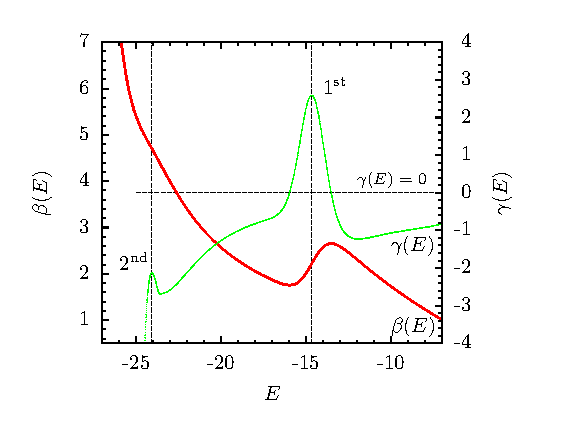
\includegraphics[width = 0.5\textwidth]{chapter7Figs/micro_example.eps}
\caption{\label{fig:Fig_1}%
Microcanonical inflection-point analysis of the
inverse microcanonical temperature $\beta(E)$. The prominent
back-bending region in $\beta(E)$, together with the positive-valued peak 
in its energy derivative $\gamma(E)$ at $E \approx -15$, indicates a 
\textit{first-order}
transition. The negative-valued peak at $E\approx -24$ corresponds
to a \textit{second-order} transition.}
\end{figure}
%
%%%%%%%%%%%%%%%%%%%%%%%%%%%%%%%%%
%%%%%%%%%%% RESULTS %%%%%%%%%%%%%%%%
%%%%%%%%%%%%%%%%%%%%%%%%%%%%%%%%%
\section{Results}
\label{sec:res}
%
%
\begin{figure}
\center
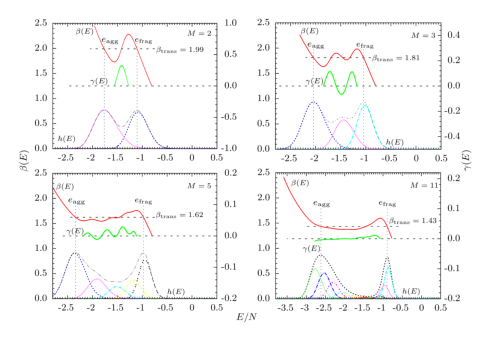
\includegraphics[width = 1.03\textwidth]{chapter7Figs/combinedMicro.eps}
\caption{\label{fig:Fig_2}Microcanonical temperature
$\beta(E)$ and its energy derivative $\gamma(E)$ for systems with $M =
2,3,5,11$ polymer chains with $N=5$ monomers each. 
The dashed vertical lines $e_{\mathrm{agg}}$ and $e_{\mathrm{frag}}$
outline the aggregation transition region. The upper horizontal dashed line
provides an estimate for the inverse 
aggregation temperature $\beta_{\mathrm{agg}}$. 
The oscillations in $\beta(E)$ reveal the sequential nature of the
transition 
and correspond to individual subtransitions.
The unimodal canonical energy histograms of the subphases
$h_{i}(\beta_{\mathrm{agg}};E)$ are shown together with the combined
histogram $h(\beta_{\mathrm{agg}};E)$. The absolute scale of these
distributions is arbitrary.}
\end{figure}
%
Previous studies of single flexible elastic homopolymers reveal the
existence
of three distinct structural phases~\cite{Schnabel2009,svbj1}. 
In the high-temperature gas-like regime, typical
conformations resemble extended, random coils. With decreasing temperature,
the system
first undergoes the $\Theta$ collapse transition into the liquid-like
compact globular phase,
and finally freezes into the solid ``crystalline'' phase. From our
simulations of the
multi-chain model employed in this study, we find that the prominent
aggregation transition is accompanied by the 
collapse of the individual chains, and the two transitions are not
separate processes. This has also
been observed in the case of semi-flexible 
homopolymers~\cite{Junghans2009}. 
However, in contrast to heteropolymer systems~\cite{Junghans2011}, the
freezing
transition occurs at temperatures well below the aggregation transition.
In fact, at low
temperatures, the thermodynamic properties of a multi-chain system
are very similar to those
of a single polymer chain with identical (total) number of monomers
$M\cdot N$. 
%%%%%%%%% Microcanonical Analysis %%%%%%%%%%%%%
\subsection{Microcanonical analysis of aggregation transitions}
%
In this section, we discuss the properties of aggregation transitions from
the perspective
of microcanonical analysis. We systematically examine systems consisting
of up to 
$M = 20$ individual chains with fixed length of $N = 5$ monomers. Brief
inspection of 
the microcanonical quantities for four system sizes in Fig.~\ref{fig:Fig_2}
suggests 
that for finite systems the aggregation transition is a first-order
process, as expected. 
The microcanonical inverse temperature curves $\beta(E)$ show a prominent
back-bending 
region accompanied by positive-valued peaks in $\gamma(E)$. The low-energy
aggregate phase is energetically separated from the disordered fragmented 
phase by an amount corresponding to the latent heat 
$\Delta q = e_{\mathrm{frag}} - e_{\mathrm{agg}}$, 
represented in Fig.~\ref{fig:Fig_2} by the separation between the two
dashed vertical lines. Finally, the combined canonical histograms $h(E)$,
also shown in Fig.~\ref{fig:Fig_2}, exhibit bimodality which is
characteristic of first-order transitions in finite systems.

Closer inspection of the back-bending region of $\beta (E)$ reveals 
additional oscillations. It is evident that their number is
proportional to the number of 
individual chains in the system. This observation motivates the description
of the aggregation transition as a series of subtransitions between
intermediate structural phases. Here we define the term ``subphase'' to
represent a distinct grouping of partially formed aggregates. As shown in
Fig.~\ref{fig:Fig_3}, a system of $M =4$ chains can form three intermediate
subphases $\{\{3,1\},\{2,2\},\{2,1,1\}\}$, where the number of elements in
each set corresponds to the number of non-interacting partial clusters, and
the numerical values represent the number of chains in each cluster.
Previous studies suggest that subtransitions occur between these partially 
fragmented subphases~\cite{jbj1,Junghans2008,Junghans2009,Junghans2011}.
However, this analysis was performed mostly on the level of 
visual inspection of individual system configurations. For a more
quantitative approach, we have implemented a structure-detection algorithm
capable of classifying configurations based on the number and size of
partially formed aggregates. This allows us to collect separate statistical
data for each subphase and to determine their relative frequency.
%
\begin{figure}
\center
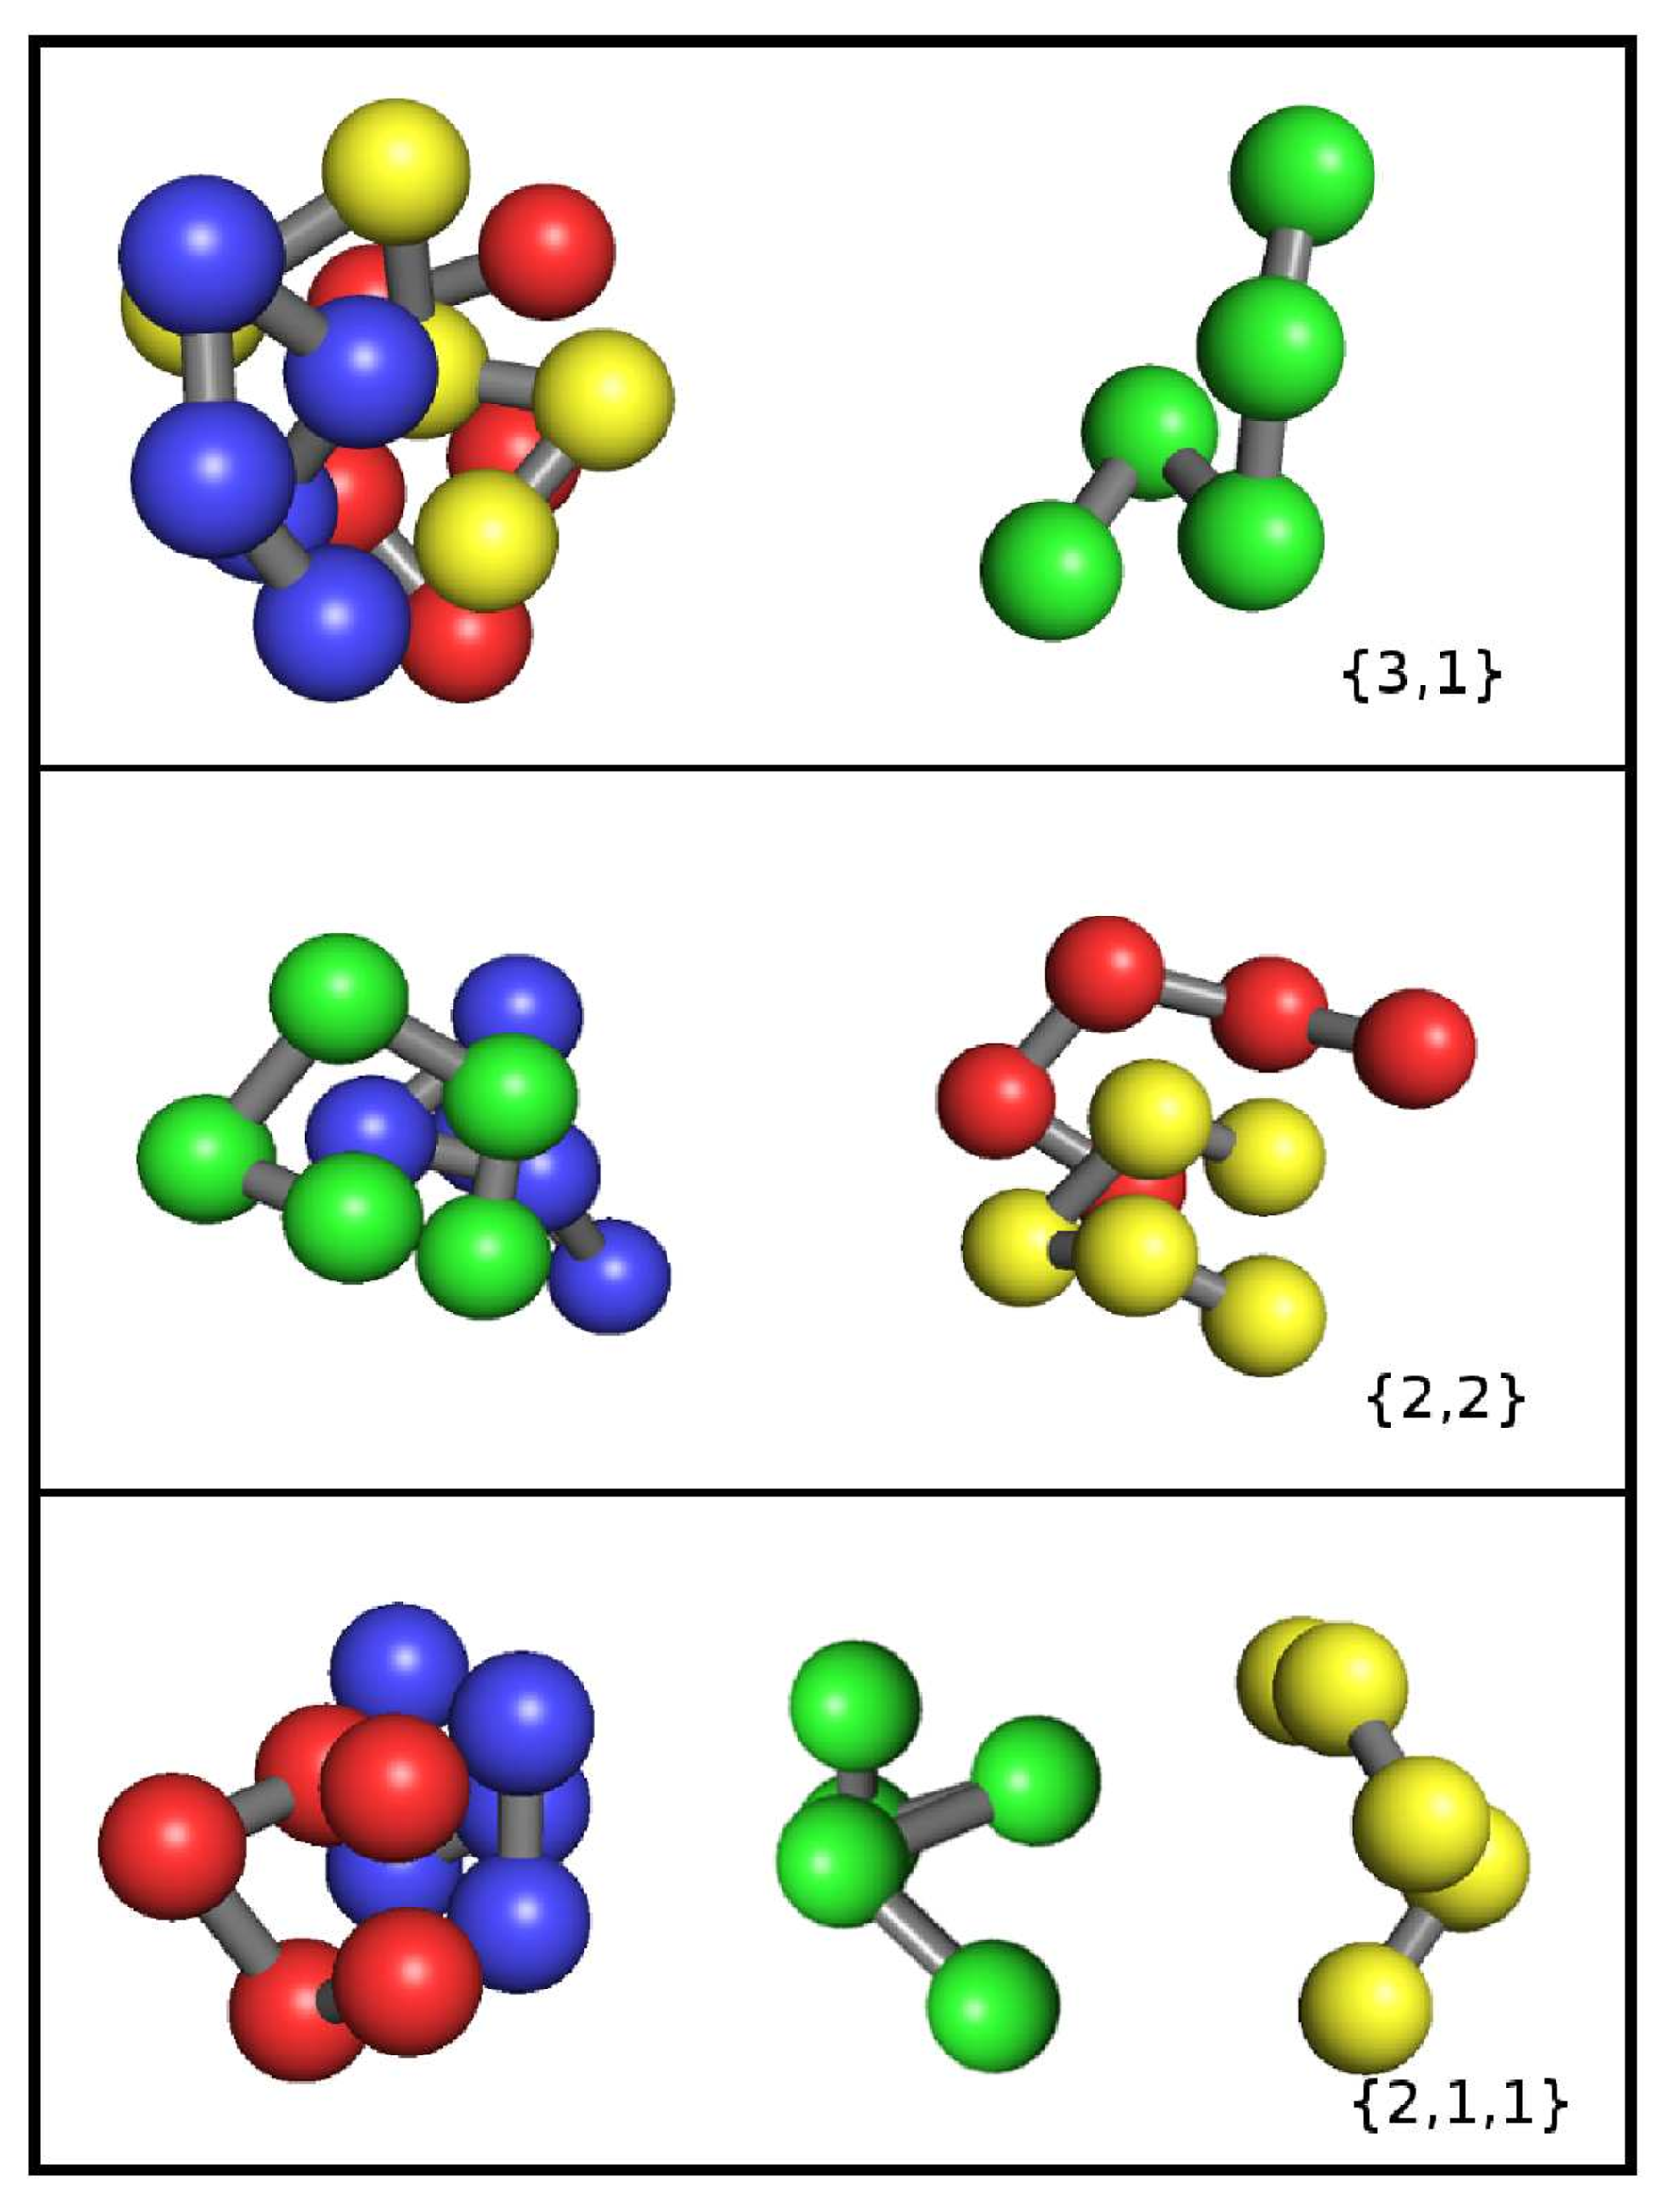
\includegraphics[width = 0.7\textwidth]{chapter7Figs/configurations.eps}
\caption{\label{fig:Fig_3} Sample configurations of
intermediate subphases found at the aggregation temperature in a system
consisting of four chains with five monomers each. Due to entropic
suppression, the $\{2,2\}$ subphase has an unexpectedly small canonical
probability 
$p_{\{2,2\}}(\beta_{\mathrm{agg}}) < 0.007$, and is the first example of a
\textit{missing} (or entropically strongly suppressed) subphase in the
aggregation process of the multi-chain system.}
\end{figure}
%
The total density of states of a system in the transition region can be
expressed as the sum of contributions from individual subphases
%
\begin{equation}
g(E) = \sum_{i} g_{i}(E).
\label{eq:densOfStates}
\end{equation}
%
The probability of finding a system in the $i$-th subphase at a fixed
energy $E$ can then be written as
%
\begin{equation}
p_{i}(E) = \frac{g_{i}(E)}{g(E)}.
\label{eq:multProb}
\end{equation}
%
The logarithm of the density of states, the microcanonical entropy $S(E)$,
cannot be expressed as a sum of individual subphase entropies. Instead
%
\begin{equation}
S(E) = k_{\mathrm{B}}\mathrm{ln}\sum_{i}e^{S_{i}(E)/k_{\mathrm{B}}},
\label{eq:micEntropy}
\end{equation}
%
where $S_{i}(E) = k_{\mathrm{B}}\mathrm{ln}\, g_{i}(E)$.
%
\begin{figure}
\center
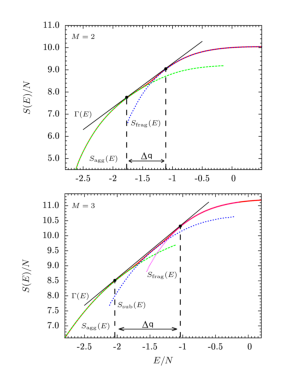
\includegraphics[width = 0.7\textwidth]{chapter7Figs/entropyCombined.eps}
\caption{\label{fig:Fig_4} Microcanonical entropy per
monomer $S(E)$ (solid)
and the individual subphase entropies (dotted) for systems with 
$M = 2,3$ polymer chains. The double-tangent $\Gamma (E)$
represents the Gibbs hull, the slope of which provides an estimate
for the inverse transition temperature $\beta_{\mathrm{agg}}$.}
\end{figure}
%
In Fig.~\ref{fig:Fig_4}, the microcanonical entropy $S(E)$~(solid) and
the individual subphase entropy curves (dashed) are shown
for systems of $M = 2$ and $M = 3$ chains. For $M=2$, aggregation 
is a single-step transition between the fragmented and the aggregate 
phase. When the aggregate is dissociated into two weakly 
interacting chains, the system gains an amount of entropy approximately
equal to the translational entropy of a single chain 
$S_{\mathrm{trans}} \sim \mathrm{ln}\,V$, where $V$ is the 
volume of the simulation sphere. This increase in entropy is apparent 
from the vertical separation between $S_{\mathrm{agg}}$ 
and $S_{\mathrm{frag}}$. The changes in conformational entropy
are negligible in comparison to the translational entropy and will
not be discussed here.  When $M = 3$, in addition to the aggregate and 
fragmented phases, a single subphase $\{2,1\}$ can be formed. As a result, 
aggregation becomes a two-step process, each decreasing the entropy
by an amount $\sim S_{\mathrm{trans}}$. We note that the entropy
curves of the individual subphases 
are strictly concave. It is the vertical displacement between the curves,
due to changes in translational entropy, that is ultimately responsible for
the origin 
of the convex intruder in the microcanonical entropy $S(E)$ and
consequently for the back-bending feature in $\beta(E)$, signaling the
first-order character of the aggregation transition. 

Differentiating Eq.~\eqref{eq:micEntropy} with respect to energy gives
a simple expression for the microcanonical inverse temperature $\beta(E)$ 
in terms of the inverse temperatures of the individual subphases:
%
\begin{equation}
\beta(E) = \frac{\sum_{i}\beta_{i}e^{S_{i}(E)/k_{\mathrm{B}}}}{
\sum_{i}e^{S_{i}(E)/k_{\mathrm{B}}}}
= \sum_{i} p_{i}(E)\beta_{i}(E).
\end{equation}
%
Hence in the transition region, $\beta(E)$ can be interpreted as the 
weighted sum of the inverse subphase temperatures with respect
to the multicanonical probabilities from Eq.~\eqref{eq:multProb}.
At a fixed energy $E$, the system can be found in one of the distinct
subphases with a respective inverse temperature $\beta_{i}(E)$. 
In general, $\beta_{i}(E) \neq \beta(E)$. However setting the energy
derivative of Eq.~\eqref{eq:multProb} to zero, we find that
$\beta_{i}(E) = \beta(E)$ precisely when the probability of a given
subphase 
$p_{i}(E)$ attains its maximum value. The oscillations in $\beta(E)$ 
arise from the changes in the relative weights $p_{i}(E)$ in
the back-bending region.

In Fig.~\ref{fig:Fig_4}, we also show the double-tangent (Gibbs hull)
$\Gamma(E)$. Its slope is the appropriate quantity for 
the estimation of the aggregation transition temperature 
$\beta_{\mathrm{agg}}$. In Table~\ref{tab:Tab_1}, $\beta_{\mathrm{agg}}$
is listed for
system sizes of up to $M = 20$ chains. In single-step first-order
transitions, 
the slope of $\Gamma(E)$ coincides with the inverse temperature obtained
by Maxwell construction. However, in composite multi-step 
transitions, the location of the Maxwell construction becomes
ambiguous due to multiple oscillations of $\beta(E)$. 
%
\begin{table}
\caption{\label{tab:Tab_1}%
Inverse aggregation temperature ($\beta_{\mathrm{agg}}$), energy per
monomer in the aggregate phase ($e_{\mathrm{agg}}$), energy per monomer in
the fragmented phase ($e_{\mathrm{frag}}$), and the latent heat per monomer
($\Delta q$). The uncertainty for all listed quantities is $\pm 0.5$ in
the last decimal.}
\begin{tabular*}{\hsize}{@{\extracolsep{\fill}}ccccc@{}}
\hline
\hline
System $(M \times N)$& $\beta_{\mathrm{agg}}$ & $e_{\mathrm{agg}}$ &
$e_{\mathrm{frag}}$ & $\Delta q$\\
\hline
$2  \times 5$  &   1.99 &  -1.77 & -1.11 & 0.67\\
$3  \times 5$  &   1.81 &  -2.04 & -1.04 & 1.00\\
$4  \times 5$  &   1.70 &  -2.22 & -1.01 & 1.22\\
$5  \times 5$  &   1.62 &  -2.35 & -0.98 & 1.37\\
$8  \times 5$   &  1.51 &  -2.56 & -0.93 & 1.63\\
$11 \times 5$  &  1.43 &  -2.62 & -0.89 & 1.73\\
$20 \times 5$  &  1.35 &  -2.80 & -0.85 & 1.95\\
\\
\hline
\hline
\end{tabular*}
\end{table}
%
\begin{table}
\caption{\label{tab:Tab_2}%
Theoretical number of subphases $(N_{\mathrm{sub}})$; not including the
fully aggregated and fragmented phases, number of significantly
represented subphases $(\hat{N}_{\mathrm{sub}})$, and the total contribution
of the ``missing'' subphases towards the canonical distribution $h(E)$ at the
inverse transition temperature $\beta_{\mathrm{agg}}$.}
\begin{tabular*}{\hsize}{@{\extracolsep{\fill}}cccc@{}}
\hline
\hline
System $(M \times N)$ & $N_{\mathrm{sub}}$ &$\hat{N}_{\mathrm{sub}}$ & $\sum p_{\mathrm{miss}}$\\
\hline
$3  \times 5$	&	1 	&	1  	& N/A\\
$4  \times 5$	&	3 	&	2  	&  $< 0.007$\\
$5  \times 5$	&	5 	&	3  	&  $< 0.014$\\
$11 \times 5$	&	54 	&	9  	&  $< 0.026$\\
$20 \times 5$	&	625 	& 	18	&  $< 0.028$\\
\\
\hline
\hline
\end{tabular*}
\end{table}
%
%%%%%%%%% Missing Subphases %%%%%%%%%%%%%
\subsection{Entropically suppressed subphases}
%
In the following, we discuss the results of the analysis of canonical 
energy histograms $h(E;\beta_{\mathrm{agg}})$, shown alongside 
the microcanonical quantities in Fig.~\ref{fig:Fig_2}. The histogram 
$h(E;\beta_{\mathrm{agg}})$, collected at the inverse aggregation
temperature $\beta_{\mathrm{agg}}$, can be expressed as a sum
of contributions from individual subphases
%
\begin{equation}
h(E;\beta_{\mathrm{agg}}) = \sum_{i}h_{i}(E;\beta_{\mathrm{agg}}),
\end{equation}  
%
where the canonical histograms of the subphases are
related to their contributions towards the density of states via
\begin{equation}
h_{i}(E;\beta_{\mathrm{agg}}) \propto g_{i}(E)e^{-\beta_{\mathrm{agg}}E}.
\end{equation}
%
At all system sizes, the aggregate and fragmented phases have the 
largest canonical probability and are energetically well separated.
The intermediate subphases have overlapping energy distributions
and occur with lower probabilities due to entropic suppression.

A striking feature emerges for systems with $M > 3$ chains.
Already for $M = 4$ (see Fig.~\ref{fig:Fig_5}), we notice that the
subphase consisting of 
two clusters $\{2,2\}$ appears with unexpectedly small canonical
probability $p_{\{2,2\}}(\beta_{\mathrm{agg}}) < 0.007$.
That only certain subphases contribute significantly 
towards the canonical energy histograms, becomes even more apparent
for larger systems. In Table~\ref{tab:Tab_2}, we list the theoretical
values for the number of possible subphases $(N_{\mathrm{sub}})$
alongside the number of subphases that were detected 
with non-negligible probability $(\hat{N}_{\mathrm{sub}})$.
The total contribution of the \textit{missing} subphases towards the
canonical
energy histograms $h(E)$ is less then $\approx 3\%$ despite 
the fact that the number of the subphases grows rapidly with system size.
The observed results suggest that a system of $M$ chains 
is most often found in a small subset of $(M-2)$ subphases, 
each consisting of $K$ individual chains and a cluster of $(M - K)$ chains.
In fact, for $M<8$ we observe $(M-1)$ oscillations in the inverse
microcanonical temperature $\beta(E)$, showing that the aggregation
transition consists of a sequence of $(M-1)$ distinct subtransitions,
each corresponding to a single chain breaking off the main aggregate. 
However in larger systems, some of the subtransitions overlap
in energy and cannot be associated with individual oscillations of 
$\beta(E)$.
%
\begin{figure}
\center
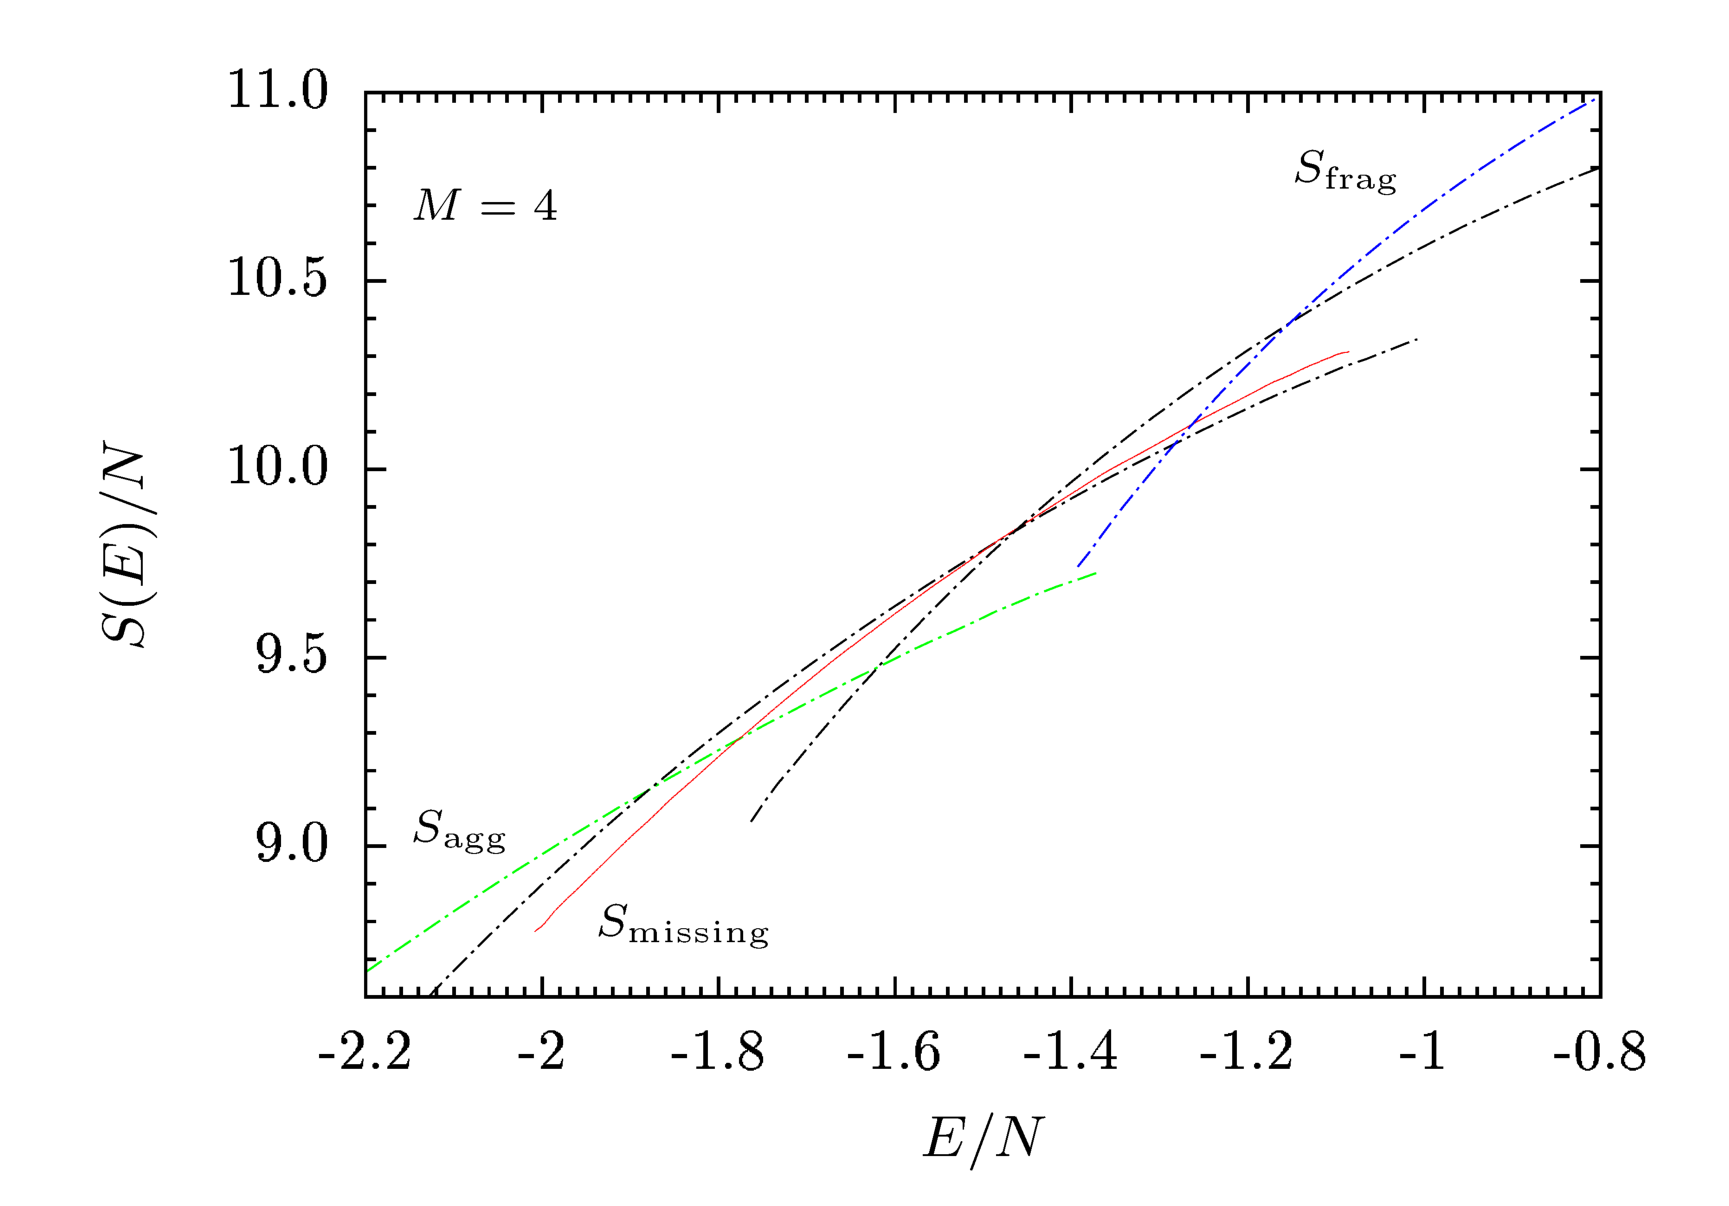
\includegraphics[width = 0.7\textwidth]{chapter7Figs/microEntropy.eps}
\caption{\label{fig:Fig_5} Subphase entropy curves (patterned) in the aggregation
transition region for a system of $M=4$ polymer chains. The entropically suppressed 
\textit{missing} subphase $\{2,2\}$ is highlighted in red (solid).}
\end{figure}
%
In order to better understand the reason behind the \textit{missing}
subphases,
we first consider the effects of energy and translational entropy 
on the relative positions of subphase entropy curves $S_{i}(E)$. 
A reduction in the number of intra-chain interactions leads to the increase
in energy, and as a result, subphases with a higher degree of 
fragmentation have their entropy curves shifted to higher energies. 
The number of independent fragments in a subphase determines its
translational entropy and largely the vertical position of its entropy
curve. 

Closer look at Eq.~\eqref{eq:micEntropy} 
reveals that only those subphases whose entropy curves 
are closest to the total entropy $S(E)$, contribute significantly. 
Therefore an increase in energy of a subphase must be 
compensated by a sufficient increase in its translational entropy.
Not surprisingly, the $(M-2)$ most frequent subphases 
consist of $K$ individual chains and a single cluster of $(M - K)$ chains,
maximizing translational entropy while maintaining a relatively high number
of 
inter-chain interactions. In Fig.~\ref{fig:Fig_5}, we provide an example
of the first missing subphase in a system of $M=4$ chains. 
It is clear that except for a very narrow energy interval,
the $\{2,2\}$ subphase is depleted by the lower-energy $\{3,1\}$ 
and the higher-entropy $\{2,1,1\}$ subphases (see Fig.~\ref{fig:Fig_3}). As
the system size
increases, the number of \textit{missing} subphases increases
rapidly, while the number of subphases with substantial canonical 
probabilities remains linearly proportional to~$M$. 
%
%%%%%%%%% Scaling Properties %%%%%%%%%%%%%
\subsection{Scaling properties}
%
\begin{figure}
\center
\includegraphics[width = 0.7\textwidth]{chapter7Figs/scalingCombined.eps}
\caption{\label{fig:Fig_6} Scaling behavior of the aggregation transition temperature
$T_{\mathrm{agg}}$ and the latent heat per monomer $\Delta q$, with respect
to $M^{-1/3}$ where $M$ is the number of polymer chains. The latent heat
increases with system size, providing further evidence that the transition
remains of 
first order even for large $M$. }
\end{figure}
%
It is also interesting to discuss the dependence of the aggregation
temperature $ T_{\mathrm{agg}} = \beta_{\mathrm{agg}}^{-1}$, and the
associated latent heat per monomer
$\Delta q = e_{\mathrm{frag}} - e_{\mathrm{agg}}$, on the system size $M$. 
Previous studies have addressed in detail the effects of system size
and the particle density $\rho$ on the transition
temperature~\cite{Zieren2014,Zieren2015}.
Here we keep the monomer density constant at $\rho = 10^{-3}$ and consider
the scaling properties of $T_{\mathrm{agg}}$ and $\Delta q$ only to obtain
further
evidence that the aggregation transition
remains
first-order-like with increasing system size. In Table~\ref{tab:Tab_1}, we
have listed the values of $\beta_{\mathrm{agg}}$ 
and $\Delta q$ for system sizes of up to $M = 20$ chains. 
Assuming that the finite-size corrections to the aggregation transition
temperature
are mainly due to volume effects, we start with the ansatz
%
\begin{equation}
T_{\mathrm{agg}} \propto \alpha_{0} + \alpha_{1}M^{-1/3}
+\mathcal{O}(M^{-2/3}).
\end{equation}
%
Due to the difference in the number of nearest-neighbor interactions
between 
surface and bulk monomers, we expect the specific heat $\Delta q$ to depend
not only on the bulk volume occupied by the system, but also on its
surface. Hence,
%
\begin{equation}
\Delta q \propto \delta_{0} + \delta_{1}M^{-1/3} + \delta_{1}M^{-2/3} + 
\mathcal{O}(M^{-1}).
\end{equation}
%
Data fits of the values from Table~\ref{tab:Tab_1} are shown in
Fig.~\ref{fig:Fig_6}. We observe
that the transition temperature is reduced for small system sizes
as finite-size effects become more prominent. For very large system sizes,
it converges to a fixed
value ($T_\mathrm{agg}^{M\to \infty}\approx 0.95$). The latent heat per
monomer approaches the estimated value $\Delta q^{M\to \infty}\approx 2.56$
in the thermodynamic limit, providing further evidence that the aggregation
transition
is a first-order phase-separation process.
%
\section{Summary}
\label{sec:sum}
%
In this study, we have investigated the properties of the aggregation
transition for systems consisting of up to $M = 20$ short flexible elastic
homopolymer chains. Utilizing the powerful tools of microcanonical
inflection point analysis, we have confirmed that the aggregation
transition is a sequential process consisting of $M-1$ subtransitions
between intermediate, partially fragmented structural phases. Each
oscillation in the microcanonical inverse temperature curve indicates a
single transition between two adjacent subphases. We have established the
relationship between the microcanonical density of states $g(E)$ and the
densities of states $g_{i}(E)$ corresponding to the individual subphases.
From this, we have further derived similar expressions for the
microcanonical entropy $S(E)$ and its energy derivative, the microcanonical
inverse temperature $\beta(E)$. We have used those relationships to
motivate the origins of the convex intruder in $S(E)$ and the prominent
back-bending region in $\beta(E)$, both of which are indicators of a
first-order process.

Canonical energy histograms $h_{i}(\beta;E)$, collected at the transition
temperature $\beta_{\mathrm{agg}}$ for each individual subphase, confirm
that certain subphases contribute only negligibly to the total canonical
distribution. The origin of these \textit{missing} subphases can be
explained on the basis of the effects of translational entropy on the 
relative positions of the subphase entropy curves $S_{i}(E)$. The results
of this study show that with increasing system size, the number of possible
subphases increases rapidly, whereas their relevant subset increases only
linearly. 

Finally, we have discussed the scaling properties of 
$\beta_{\mathrm{agg}}$ and the latent heat per monomer $\Delta q$. The
increasing values of $\Delta q$ with system size provide further evidence
that the aggregation transition remains a first-order process even as $M$
tends towards the thermodynamic limit. 

\chapter{Summary and Outlook}









%~~~~~~~~~~~~~~~~ Reference ~~~~~~~~~~~~~~~~~~%
\addcontentsline{toc}{chapter}{Bibliography}
\begin{thebibliography}{99}
        %%%%%%%%%%% CHAPTER 2 %%%%%%%%%%%%%%%%%%
\bibitem{Bachmann2014}
M.~Bachmann, \emph{Thermodynamics and Statistical Mechanics of
Macromolecular Systems}, (Cambridge University Press, Cambridge,
2014).
%
\bibitem{Rugh2001}
H.~H.~Rugh , Phys.\ Rev.~E \textbf{64},
055101 (2001).

%%%%%%%%%%% Microcanonical Ensemble %%%%%%%%%%%

\bibitem{Kardar2007}
M.~Kardar, \emph{Statistical Physics of Particles}, (Cambridge University Press, New York, 2007).
%
\bibitem{Pathria}
R.~K.~Pathria, and P.~D.~Beale, \emph{Statistical Mechanics}, (Elsevier, Oxford, 2011).
%
\bibitem{Sethna2006}
J.~P.~Sethna, \emph{Statistical Mechanics: Entropy, Order Parameters, and Complexity}, 
(Oxford University Press, New York, 2006).
%


%%%%%%%%%%% Microcanonical Analysis %%%%%%%%%%%%
\bibitem{Gross2001} 
D.~H.~E.~Gross, \emph{Microcanonical Thermodynamics}, (World Scientific, Singapore,  2001).
%
\bibitem{Stevenson}
P.~M.~Stevenson, Phys.\ Rev.~D \textbf{23}, 2916 (1981).
%
\bibitem{Schnabel2011}
S.~Schnabel, D.~T.\ Seaton, D.~P.\ Landau, and M.~Bachmann, Phys.\ Rev.~E
\textbf{84}, 011127 (2011). 
%


%%%%%%%%%%% Canonical Analysis %%%%%%%%%%%%%%%%

\bibitem{Landau2000}
D.~P.\ Landau, and K.~Binder, \emph{A Guide to Monte Carlo Simulations in Statistical Physics}, (Cambridge University Press, Cambridge, 2000).

%%%%%%%%%%% Definitions of Density of States %%%%%%%%%

\bibitem{Calvo1995}
F.~Calvo, and P.~Labastie,  Chem.\ Phys.\ Lett. \textbf{247}, 395 (1995).
%




\end{thebibliography}


\end{document}


